\documentclass[
a4paper,
fontsize=10pt, % Base font size
twoside=false, % Use different layouts for even and odd pages (in particular, if twoside=true, the margin column will be always on the outside)
% open=any, % If twoside=true, uncomment this to force new chapters to start on any page, not only on right (odd) pages
% chapterprefix=true, % Uncomment to use the word "Chapter" before chapter numbers everywhere they appear
% chapterentrydots=true, % Uncomment to output dots from the chapter name to the page number in the table of contents
numbers=auto, % Comment to output dots after chapter numbers; the most common values for this option are: enddot, noenddot and auto (see the KOMAScript documentation for an in-depth explanation)
% draft=true, % If uncommented, rulers will be added in the header and footer
fontmethod = modern,
% overfullrule=true, % If uncommented, overly long lines will be marked by a black box; useful for correcting spacing problems
]{kaobook}

% Choose the language
\usepackage{polyglossia}
\setmainlanguage{italian}
\usepackage[english=british]{csquotes}	% English quotes

% Creative commons license
\usepackage[
	type={CC},
	modifier={by-sa},
	version={4.0},
]{doclicense}


% Load the bibliography package
\usepackage[sorting=nyt]{kaobiblio}
\addbibresource{compilatori.bib} % Bibliography file

%\usepackage[framed=true]{kaotheorems}
\usepackage{amsmath} % Improved mathematics
\usepackage{amsthm} % Mathematical environments
\usepackage{thmtools} % Theorem styles
\usepackage[framemethod=TikZ]{mdframed}
% From kaobook
\mdfsetup{skipabove=\topskip,skipbelow=-.5\topskip}
\mdfdefinestyle{mdfkao}{
  skipabove=\topskip,
  skipbelow=\topskip, % Does not work :(
  rightmargin=0pt,
  leftmargin=0pt,
  innertopmargin=7pt,
  innerbottommargin=7pt,
  innerrightmargin=7pt,
  innerleftmargin=7pt,
  topline=false,
  bottomline=true,
  rightline=false,
  leftline=false,
  frametitlerule=true,
}

\declaretheoremstyle[
spaceabove=6pt,
spacebelow=6pt,
headfont=\normalfont\bfseries,
notefont=\mdseries, notebraces={(}{)},
bodyfont=\normalfont,
postheadspace=1em,
shaded={bgcolor=Goldenrod!45!white},
headpunct={}
]{mythmstyle}

\theoremstyle{mythmstyle}
\declaretheorem[
name=Teorema,
style=mythmstyle,
refname={Teorema,Teoremi},
Refname={Teorema,Teoremi},
numberwithin=chapter,
]{theorem}
\declaretheorem[
name=Proposizione,
style=mythmstyle,
sibling=theorem,
refname={Proposizione,Proposizioni},
Refname={Proposizione,Proposizioni},
numberwithin=chapter,
]{proposition}
\declaretheorem[
name=Corollario,
style=mythmstyle,
sibling=theorem,
refname={Corollario,Corollari},
Refname={Corollario,Corollari},
numberwithin=chapter,
]{corollary}
\declaretheorem[
name=Lemma,
style=mythmstyle,
sibling=theorem,
refname={Lemma,Lemmi},
Refname={Lemma,Lemmi},
numberwithin=chapter,
]{lemma}
\declaretheorem[
name=Nota,
style=mythmstyle,
sibling=theorem,
refname={Nota,Note},
Refname={Nota,Note},
numberwithin=chapter,
]{observation}


% Quello che segue non ha la stessa numerazione di teoremi, lemmi, ecc.
\declaretheoremstyle[
spaceabove=6pt,
spacebelow=12pt,
headfont=\normalfont\bfseries,
notefont=\mdseries, notebraces={(}{)},
bodyfont=\normalfont,
postheadspace=1em,
shaded={bgcolor=green!15!white},
headpunct={}
]{mydefstyle}
\declaretheorem[
name=Definizione,
style=mydefstyle,
refname={Definizione,Definizioni},
Refname={Definizione,Definizioni},
numberwithin=chapter,
]{definition}

\declaretheorem[
name=Problema,
style=mydefstyle,
refname={Problema,Problemi},
Refname={Problema,Problemi},
]{problem}



\declaretheoremstyle[
spaceabove=6pt,
spacebelow=6pt,
headfont=\normalfont\bfseries,
notefont=\mdseries, notebraces={(}{)},
bodyfont=\normalfont,
postheadspace=1em,
shaded={bgcolor=gray!15!white},
headpunct={}
]{myexamplestyle}
\declaretheorem[
name=Esempio,
style=myexamplestyle,
refname={Esempio,Esempi},
Refname={Esempio,Esempi},
numberwithin=chapter,
]{example}

\declaretheorem[
name=Esercizio,
style=mythmstyle,
refname={Esercizio,Esercizi},
Refname={Esercizio,Esercizi},
numberwithin=chapter,
]{exercise}


\usepackage{subfiles}

\newcommand{\parte}[1]{\pagelayout{wide}\addpart{#1}\pagelayout{margin}}


\usepackage{kaorefs}

% Set the paths where to look for images
\usepackage{subcaption}
\graphicspath{{./imgs/}{./img/}}

\makeindex[columns=3, title=Alphabetical Index, intoc] % Make LaTeX produce the files required to compile the index

\makeglossaries% Make LaTeX produce the files required to compile the glossary
\makenomenclature

% Tikz
\usetikzlibrary{automata,positioning}

\newcommand{\keyword}[1]{\textbf{#1}\marginnote{#1}}

% Produzioni
\usepackage{stackrel}
\newcommand{\sprod}[1]{\ensuremath{\stackrel[#1]{}{\Longrightarrow}}}
\newcommand{\eprod}[1]{\ensuremath{\xRightarrow[#1]{*}}}
\newcommand{\prodgen}{\ensuremath{\alpha\to\beta}\xspace}


% Grammatiche
\newcommand{\gramm}{\ensuremath{G=\langle V, T, P, S \rangle}\xspace}


\usepackage{upref}
\usepackage{siunitx}
\usepackage{upquote}
\let\refeq\relax
\usepackage{mathtools}
\usepackage{unicode-math}


%%% Local Variables:
%%% mode: LaTeX
%%% TeX-engine: luatex
%%% TeX-master: "libro-linguaggi"
%%% End:


\begin{document}

\definecolor{shadecolor}{gray}{0.80}

\titlehead{Linguaggi, Grammatiche, Parser}
\subject{}

\title[Linguaggi, Grammatiche, Parser]{Linguaggi, Grammatiche, Parser}
\subtitle{Un libro su: Linguaggi, Grammatiche, Parser}

%\author[GDV]{Gianluca Della Vedova}
\date{\today}


%----------------------------------------------------------------------------------------

\frontmatter % Denotes the start of the pre-document content, uses roman numerals

%----------------------------------------------------------------------------------------
%       OPENING PAGE
%----------------------------------------------------------------------------------------

%\makeatletter
%\extratitle{
%       % In the title page, the title is vspaced by 9.5\baselineskip
%       \vspace*{9\baselineskip}
%       \vspace*{\parskip}
%       \begin{center}
%               % In the title page, \huge is set after the komafont for title
%               \usekomafont{title}\huge\@title
%       \end{center}
%}
%\makeatother



%----------------------------------------------------------------------------------------
%       OUTPUT TITLE PAGE AND PREVIOUS
%----------------------------------------------------------------------------------------

% Note that \maketitle outputs the pages before here

\maketitle

%----------------------------------------------------------------------------------------
%       COPYRIGHT PAGE
%----------------------------------------------------------------------------------------


\vfill

\doclicenseThis%
Sei libero di riprodurre, distribuire, comunicare al pubblico, esporre
in pubblico, rappresentare, eseguire, recitare e modificare quest'opera
alle seguenti condizioni:
\begin{itemize}
\item
Attribuzione — Devi attribuire la paternit{\`a} dell'opera nei modi
indicati dall'autore o da chi ti ha dato l'opera in licenza e in modo tale da
non suggerire che essi avallino te o il modo in cui tu usi l'opera.
\item
Condividi allo stesso modo — Se alteri o trasformi quest'opera, o se
la usi per crearne un'altra, puoi distribuire l'opera risultante solo con
una licenza identica o equivalente a  questa.
\end{itemize}
%  \vspace*{1cm}

Tutto il materiale si trova al link
\url{https://github.com/gdv/linguaggi-formali}.
Tutti sono invitati a contribuire a questo libro.
\newpage
%----------------------------------------------------------------------------------------
%       PREFACE
%----------------------------------------------------------------------------------------

%\input{chapters/preface.tex}
%\index{preface}


%----------------------------------------------------------------------------------------
%       TABLE OF CONTENTS & LIST OF FIGURES/TABLES
%----------------------------------------------------------------------------------------

\begingroup % Local scope for the following commands

% Define the style for the TOC, LOF, and LOT
%\setstretch{1} % Uncomment to modify line spacing in the ToC
%\hypersetup{linkcolor=blue} % Uncomment to set the colour of links in the ToC
\setlength{\textheight}{230\hscale} % Manually adjust the height of the ToC pages

% Turn on compatibility mode for the etoc package
\etocstandarddisplaystyle % "toc display" as if etoc was not loaded
\etocstandardlines % "toc lines as if etoc was not loaded

\tableofcontents % Output the table of contents

\endgroup

%----------------------------------------------------------------------------------------
%       MAIN BODY
%----------------------------------------------------------------------------------------

\mainmatter % Denotes the start of the main document content, resets page numbering and uses arabic numbers
\setchapterstyle{kao} % Choose the default chapter heading style

\parte{Introduzione}
\chapter{Introduzione}

Questo testo si prefigge di introdurre i linguaggi formali e descrivere la
rilevanza che questi hanno nel disegno di un compilatore.

In sintesi, un compilatore è un programma che riceve il codice sorgente di un
programma e produce un programma equivalente, detto codice oggetto, in un altro
linguaggio di programmazione: spesso in assembler.

L'anatomia di un compilatore individua tre componenti
principali~\sidecite{engineering-a-compiler}:
\begin{enumerate}
\item
      Frontend: trasforma il codice sorgente in una rappresentazione intermedia
      (IR) indipendente dal linguaggio di programmazione.
\item
      Optimizer: manipola la rappresentazione intermedia per migliorarne le
      caratteristiche (rendere più veloce il programma, usare meno memoria,
      ecc.)
\item
      Backend: riceve la rappresentazione intermedia ed emette il corrispondente
      codice oggetto.
\end{enumerate}

Vedremo che i linguaggi formali sono il fondamento di ogni frontend.

%%% Local Variables:
%%% mode: LaTeX
%%% TeX-master: "../libro-linguaggi"
%%% End:



\parte{Linguaggi e grammatiche}\label{part:linguaggi}
\setchapterpreamble[u]{\margintoc}
\chapter{Linguaggi e Grammatiche}\label{cha:linguaggi+grammatiche}
\labch{Linguaggi e Grammatiche}

\section{Linguaggi}
iIniziamo con le definizioni di base che saranno fondamentali in tutto il testo.

Un \textbf{simbolo} o \textbf{carattere} è un qualsiasi oggetto.


\begin{definition}[Alfabeto]\label{def:alfabeto}
Un \keyword{alfabeto}, normalmente indicato con $\Sigma$, è un insieme finito e non vuoto di simboli.
\end{definition}

Esempi di alfabeti sono \texttt{abcdefghijklmnopqrstuvwxyz}, e l'insieme di cifre \texttt{0123456789}.
Siccome un alfabeto è un insieme, l'ordine dei simboli non è rilevante.
In altre parole \texttt{9876543210} è sempre l'alfabeto delle cifre.
Nel seguito useremo $\Sigma_{L}$ per indicare l'alfabeto delle lettere minuscole, $\Sigma_{C}$ per l'alfabeto delle cifre,
$\Sigma_{B}$ per l'alfabeto delle cifre binarie.


La giustapposizione (o concatenazione) di simboli permette di creare parole o stringhe, quali ad
esempio \texttt{parola} o \texttt{2301}.
La concatenazione di due simboli viene rappresentata semplicemente scrivendo un simbolo dopo l'altro.


\begin{definition}[Parola]\label{def:parola}
Sia $\Sigma$ un alfabeto.
Allora una \keyword{parola} è una sequenza $\sigma_{1}\cdots\sigma_{n}$ di simboli, non necessariamente
distinti, dell'alfabeto $\Sigma$.
Una parola viene normalmente rappresentata tramite la giustapposizione dei
simboli che compongono la sequenza, rispettando l'ordine.
\end{definition}

Normalmente usiamo le ultime lettere dell'alfabeto latino (ad esempio $w$, $x$,
$y$, $z$) per rappresentare parole.
La \keyword{lunghezza} di una parola è il numero di simboli nella sequenza.
La lunghezza della parola $z$ viene indicata con $|z|$.

Alcuni simboli sono speciali perchè hanno un significato particolare e non fanno parte di nessun alfabeto $\Sigma$.
Il primo simbolo speciale che vediamo è $\epsilon$ e rappresenta la stringa vuota,
formata dalla sequenza di zero simboli.

\begin{definition}[Linguaggio]\label{def:linguaggio}
Dato un alfabeto $\Sigma$, un \keyword{linguaggio} $L$ è un insieme di parole su $\Sigma$.
\end{definition}

Sebbene l'alfabeto sia finito, un linguaggio potrebbe contenere un numero
infinito di parole.
Diventa quindi importante capire quando un linguaggio infinito ha una
rappresentazione finita.
Notare che praticamente tutti i linguaggi rilevanti sono infiniti, ma con
rappresentazione finita.
Prendiamo ad esempio JSON: abbiamo una specifica formale (quindi una sequenza di
caratteri corrisponde ad un documento JSON se e solo se soddisfa la specifica),
e l'insieme dei documenti JSON è infinito.

\begin{example}\label{exa:numeri}
Un numero è formato da una parte intera che consiste unicamente di cifre e,
opzionalmente, da una parte frazionaria che consiste unicamente di cifre.
Se la parte frazionaria esiste, allora la parte intera e la parte frazionaria
sono separate da un punto.
La parte intera non può iniziare con \texttt{0} e la parte frazionaria non può
finire con \texttt{0}.
L'insieme di tutti i numeri è un linguaggio (infinito).
\end{example}

La descrizione nell'\cref{exa:numeri} è di natura insiemistica:  il
linguaggio è visto come l'insieme delle parole che lo compongono.
Quando vogliamo studiare un linguaggio, esistono tre punti di vista alternativi: (1) considerare come sia possibile generare
tutte le parole di un linguaggio, (2) descrivere una procedura che determini se
una parola appartiene al linguaggio, (3) fornire una proprietà che è soddisfatta da tutte e sole le parole del linguaggio.
Si noti che la definizione di linguaggio non cambia.
Nel seguito vedremo come questi tre punti di vista si complementino e
interagiscono fra loro.

L'approccio, basato sulla procedura per determinare se una parola
appartiene al linguaggio, ci porta a definire il primo fondamentale problema
computazionale, detto problema dell'\keyword{appartenenza} ad un linguaggio.


\begin{problem}[Appartenenza]\label{pb:appartenenza}
Siano $L$ un linguaggio e $z$ una parola, entrambi sull'alfabeto $\Sigma$.
Determinare se $z$ \keyword{appartiene} a $L$ o, in altre parole, se $z$ sia una parola del linguaggio $L$.
\end{problem}

Il problema dell'appartenenza è un \keyword{problema di decisione}, perchè
ammette solo due risposte: sì o no.
La nozione di  concatenazione non si applica solo ai caratteri, ma anche a stringhe e linguaggi.


\begin{definition}[Concatenazione]\label{def:concatenazione-parole}
Siano $w$ e $x$ due parole.
La loro \keyword{concatenazione} $wx$ è ottenuta prendendo $w$ e facendo seguire a questa la stringa  $x$.
Più formalmente, se $w=a_{1}\cdots a_{|w|}$ e $x=b_{1}\cdots b_{|w|}$, allora la loro concatenazione $wx$ è la stringa
$a_{1}\cdots a_{|w|} b_{1}\cdots b_{|w|}$.
\end{definition}

\begin{definition}[Concatenazione di linguaggi]\label{def:concatenazione-linguaggi}
Siano $L_{1}$ e $L_{2}$ due linguaggi, rispettivamente su alfabeto $\Sigma_{1}$ e $\Sigma_{2}$.
Allora la loro concatenazione $L_{1}L_{2}$ è uguale alla concatenazione di tutte le coppie ordinate di parole di $L_{1}$
e $L_2$.
Formalmente, $L_{1}L_{2} = \{ w_{1}w_2 : w_{1}\in L_{1}, w_{2}\in L_2\}$.
\end{definition}

Una definizione equivalente di concatenazione di linguaggi è $L_{1}L_{2} = \{ w_{1}w_2 : (w_{1}, w_{2})\in L_{1} \times L_2\}$.
Si noti anche che l'alfabeto del linguaggio $L_1 L_2$ è $\Sigma_{1} \cup \Sigma_{2}$.


\begin{definition}\label{def:potenza-linguaggio}
Sia $L$ un linguaggio e sia $k$ un numero intero strettamente positivo.
Allora la $k$-esima \keyword{potenza} di $L$, denotata con $L^k$, è l'insieme di tutte le stringhe ottenute concatenando
$k$ parole, non necessariamente distinte, del linguaggio $L$.
\end{definition}

Per convenzione, si indica con $L^{0} = \{ epsilon \}$.
Quindi possiamo vedere $L^{1} =L$, mentre $L^{k} = L^{k-1} \Sigma$ se $k>1$.
Una variante della \cref{def:concatenazione-linguaggi} consiste nella definizione di potenza di un alfabeto.

\begin{definition}\label{def:potenza-alfabeto}
Sia $\Sigma$ un alfabeto e sia $k$ un numero intero strettamente positivo.
Allora la $k$-esima \keyword{potenza} di $\Sigma$, denotata con $\Sigma^k$, è l'insieme di tutte le stringhe di
lunghezza $k$ sull'alfabeto $\Sigma$.
\end{definition}

Per convenzione, si indica con $\Sigma^{0} = \{ \epsilon \}$, esattamente come nel caso di potenza di un linguaggio.
Vediamo $\Sigma^{1}$ come il linguaggio formato da tutte le parole di lunghezza $1$ prese dall'alfabeto
$\Sigma$, mentre $\Sigma^{k} = \Sigma^{k-1} \Sigma$ se $k>1$.
Non possiamo dire $\Sigma^{1} = \Sigma$ perchè il primo è un insieme di parole e il secondo è un
insieme di simboli.

\begin{example}\label{exa:L3}
L'alfabeto $\Sigma_{B}^{3}$ è formato dalle stringhe \texttt{000}, \texttt{001}, \texttt{010}, \texttt{011}, \texttt{100}, \texttt{101}, \texttt{110}, \texttt{111}.
\end{example}


La nozione di chiusura permette di generalizzare la potenza al caso $k=\infty$.




\begin{definition}\label{def:punto-fisso}
Sia $A$ un insieme non vuoto e sia $\phi$ una funzione con mappa insiemi in insiemi.
Allora $A$ è un \keyword{punto fisso} per $\phi$ se $\phi(A) \subseteq A$.
\end{definition}

In altre parole, $A$ è un punto fisso se l'applicazione di $\phi$ non ``cambia'' $A$.
Ovviamente una funzione $\phi: X\mapsto Y$ potrebbe non avere punti fissi e potrebbe anche avere più di un punto fisso.
Noi siamo interessati ai \emph{minimi punti fissi} che contengono un insieme $A$: i più piccoli insiemi $B\supseteq A$
tali che $B$ sia un punto fisso per $\phi$.

\begin{definition}\label{def:kleene}
Sia $\Sigma$ un alfabeto.
Allora la sua \keyword{chiusura di Kleene}, denotata con $\Sigma^{*}$, è l'unione infinita di potenze
$\bigcup_{k=0}^{\infty} \Sigma^k = \Sigma^0 \cup \Sigma^1 \cup \cdots$.
\end{definition}

\begin{proposition}\label{prop:kleene-punto-fisso}
Sia $\Sigma$ un alfabeto.
Allora $\Sigma^{*}$ è il minimo punto fisso di $\Sigma \cup \{\epsilon\}$ rispetto alla funzione
chiusura di Kleene come minimo punto fisso di $L\cup \{\epsilon\}$ rispetto alla funzione $\phi$ che mappa ogni
linguaggio $L$ in $\phi(L) = L^{2}$.
\end{proposition}

\begin{example}\label{exa:chiusura-kleene}
$\Sigma_{B}^{*} = \{\mathtt{\epsilon},\mathtt{0},\mathtt{1},\mathtt{00},\mathtt{01},\mathtt{10},\mathtt{100},\mathtt{000},\ldots \}$.
\end{example}

Adesso possiamo introdurre la notazione più utilizzata per specificare un linguaggio costruito su un determinato alfabeto.


\begin{observation}\label{obs:linguaggio}
Un linguaggio $L$ su alfabeto $\Sigma$ è un sottoinsieme di stringhe in $ \Sigma^*$,
quindi $L\subseteq \Sigma^*$.
\end{observation}

Siccome ogni linguaggio è un insieme, il simbolo $\emptyset$ denota anche il \keyword{linguaggio vuoto} (notare che
$\emptyset\in\Sigma^k,\,|\emptyset|=0$), che è
diverso dal linguaggio $\{\epsilon\}$ che consiste esattamente della stringa vuota.
Infatti $|\{\varepsilon\}|=1$.
Infine si noti che $\Sigma^*$ è sempre un insieme infinito.
Vediamo adesso alcuni esempi di linguaggi sull'alfabeto $\Sigma_{B}$.


\begin{example}\label{exa:0n01}
Le stringhe che consistono in $n$ \texttt{0} seguiti da $n$ \texttt{1}:
$\{\varepsilon,\mathtt{01},\mathtt{0011},\mathtt{000111},\ldots\}$.
\end{example}

\begin{example}\label{exa:0=1}
le stringhe con un uguale numero di 0 e di 1:
$\{\varepsilon,\mathtt{01},\mathtt{10},\mathtt{0011},\mathtt{0110},\mathtt{0101},\mathtt{1001},\ldots\}$.
\end{example}

\begin{example}\label{exa:numeri-primi-binari}
le stringhe che codificano un numero primo:
$\{\mathtt{10},\mathtt{11},\mathtt{101}, \mathtt{111}, \ldots\}$.
\end{example}

\begin{example}\label{exa:numeri-primi-unari}
le stringhe che sono una codifica unaria di un numero primo, senza usare \texttt{0}:
$\{\mathtt{11},\mathtt{111},\mathtt{11111}, \mathtt{1111111}, \ldots\}$.
\end{example}

L'\cref{exa:numeri-primi-unari} è interessante perchè l'alfabeto effettivamente usato ha un solo simbolo.
In altre parole, non sono necessari due simboli per le nozioni di alfabeto e linguaggio.


\begin{observation}\label{obs:linguaggi-banali}
Sia $\Sigma$ un alfabeto.
Allora $\emptyset$, $\{\varepsilon\}$, e $\Sigma^{k}$ per ogni intero $k\ge 1$ sono tutti linguaggi per l'alfabeto $\Sigma$.
\end{observation}

Notiamo che tutti gli esempi di linguaggi che abbiamo dato in questa sezione sono basati sulla descrizione di una
proprietà che è vera per tutte e sole le parole del linguaggio.
Questo vuole dire che stiamo considerando una visione \emph{insiemistica} dei linguaggi.
Vedremo presto che questa non è l'unica visione possibile.


\section{Grammatiche}\label{sec:grammatiche}

Mentre la \ref{def:linguaggio} vede un linguaggio come un insieme, in questa sezione andiamo ad introdurre il concetto
di grammatica: ciò ci porterà a vedere come sia possibile \emph{generare} tutte e sole le parole appartenenti ad un linguaggio.


\begin{definition}[Grammatica]\label{def:grammatica}
Una \keyword{grammatica} $G$ è una quadrupla $G=\langle V, T, P, \mathsf{S} \rangle$ dove:
\begin{itemize}
	\item $V$ è un insieme finito di \keyword{variabili} o non terminali;
	\item $T$ è un insieme finito di simboli \keyword{terminali}, ovvero i simboli dell'alfabeto di riferimento,
	  disgiunto dalle variabili.
Quindi $V \cap T=\emptyset$;
	\item $P$ è un insieme finito di \textbf{produzioni} o regole;
	\item $\mathsf{S}\in V$ è il \keyword{simbolo iniziale} ($\mathsf{S}$ rappresenta ``start'').
\end{itemize}
\end{definition}


Dobbiamo ancora fornire la definizione di produzione.

\begin{definition}\label{def:produzione}
Una \keyword{produzione} $\alpha \to \beta$ formata da tre parti:
\begin{itemize}
\item una stringa non vuota $\alpha$, detta \keyword{testa},  sull'alfabeto $V \cup T$,
	  \item il simbolo $\to$ della produzione;
\item una stringa $\beta$, detta \keyword{corpo},  sull'alfabeto $V \cup T$.
\end{itemize}
\end{definition}

Notiamo che sia la testa che il corpo di una produzione possono contenere sia terminali che variabili, senza alcuna
restrizione: possono quindi esserci solo terminali, solo variabili, oppure entrambi.
Anche l'ordine con cui appaiono non ha vincoli.
L'unica restrizione è che la testa non può essere la stringa vuota, mentre il corpo potrebbe essere la stringa vuota
($\beta = \epsilon$).
Convenzionalmente, per evitare ambiguità, il simbolo di produzione $\to$ non appartiene a $V\cup T$.


Ad ogni grammatica $G=\langle V, T, P, S \rangle$ possiamo associare il linguaggio generato da $G$.
Intuitivamente, si parte dal simbolo iniziale $S$ e si applica ripetutamente una produzione.
L'applicazione di una produzione $\alpha\to\beta$ consiste nell'individuare $\alpha$ nella sottostringa attuale e
sostituirla con $\beta$.
Dopo ogni applicazione si ottiene una nuova stringa attuale e il processo può ripetersi, anche applicando una produzione
diversa da quella utilizzata nel passo precedente.
Quando la stringa attuale è formata da soli simboli terminale, tale stringa è una delle parole del linguaggio.
Il processo di ripetute applicazioni di produzioni si chiama derivazione.

Per semplificare alcune parti, introduciamo la definizione di forma sentenziale.

\begin{definition}[Forma sentenziale]\label{def:forma-sentenziale}
Sia \gramm una grammatica.
Una \keyword{forma sentenziale} è una stringa sull'alfabeto $V\cup T$.
\end{definition}


\begin{example}\label{exa:0001}
Consideriamo il linguaggio $L$ su alfabeto $\Sigma_{B}$ delle parola che contengono esattamente un \texttt{1} e questo
carattere is deve trovare in ultima posizione.
Una grammatica $G=\langle V, T, P, S \rangle$ che genera il linguaggio $L$ ha $V=\{\mathsf{Z}, \mathsf{U}\}$,
$T=\{\mathtt{0}, \mathtt{1}\}$, e le produzioni $\mathsf{S}\to \mathsf{Z}\mathsf{U}$, $\mathsf{S}\to \mathsf{U}$,
$\mathsf{U}\to \mathtt{1}$, $\mathsf{Z}\to \mathsf{Z}\mathtt{0}$, and $\mathsf{Z}\to \mathtt{0}$.
\end{example}

Possiamo notare che la stringa \texttt{001} viene generata dalla grammatica $G$ tramite la seguente sequenza di
applicazioni di produzione:

\[\mathsf{S} \sprod{\mathsf{S}\to \mathsf{Z}\mathsf{U}} \mathsf{Z}\mathsf{U}  \sprod{\mathsf{Z}\to \mathsf{Z}\mathtt{0}} \mathsf{Z}\mathtt{0}\mathsf{U} \sprod{\mathsf{U}\to \mathtt{1}} \mathsf{Z}\mathtt{0}\mathtt{1} \sprod{\mathsf{Z}\to \mathtt{0}} \mathtt{0}\mathtt{0}\mathtt{1} \]

Questa derivazione non è l'unica possibile per generare la stringa \texttt{001} e la grammatica $G$ che abbiamo
descritto non è l'unica in grado di generare il linguaggio $G$.
Possiamo adesso dare la definizione formale di applicazione di una produzione.

\begin{definition}Applicazione di una produzione\label{def:applicazione-produzione}
Siano $\alpha$, $\beta$, $\gamma$, $\delta$ stringhe su alfabeto $V\cup T$.
Sia $\gramm$ una grammatica e sia \prodgen una sua produzione (quindi $\alpha\neq\epsilon$).
L'\keyword{applicazione} della produzione \prodgen alla stringa $\gamma\alpha\delta$ è denotata con
$\gamma\alpha\delta \sprod{\prodgen} \gamma\beta\delta$ e rappresenta il fatto che $\alpha$ viene sostituita con $\beta$.
Se la produzione \prodgen è facilmente identificabile, oppure se non ci interessa specificare la produzione usata, possiamo denotare l'applicazione indicando solo la grammatica $G$
con $\gamma\alpha\delta \sprod{G} \gamma\beta\delta$.
Se anche la grammatica coinvolta non è ambigua, possiamo ometterla usando la scrittura $\gamma\alpha\delta \sprod{} \gamma\beta\delta$.
\end{definition}

Per denotare in modo compatto l'effetto di una sequenza di applicazioni di produzioni, e definire il linguaggio generato
da una grammatica, introduciamo il concetto di
produzione estesa.

\begin{definition}[Applicazione estesa di una produzione]\label{def:applicazione-produzione-estesa}
Sia $\gramm$ una grammatica e siano $\alpha$, $\beta$ due forme sentenziali di $G$.
Allora possiamo scrivere $\alpha \eprod{G} \beta$ se esiste una sequenza
$\langle \gamma_{1}, \ldots, \gamma_{n}\rangle $ di $n$ forme sentenziali tali che $\alpha = \gamma_{1}$,
$\beta = \gamma_{n}$, e $\gamma_{i} \sprod{G} \gamma_{i+1}$ per ogni $1\le k< n$.
In questo caso diciamo che $\beta$ è il risultato dell'\keyword{applicazione estesa} di produzioni di $G$ alla stringa $\alpha$.
\end{definition}


\begin{definition}[linguaggio generato]\label{def:linguaggio-generato}
Sia \gramm una grammatica.
Il \keyword{linguaggio generato} da $G$, denotato con $L(G)$ è l'insieme $L(G)= \{ w\in T^{*}: S \eprod{G} w\}$.
\end{definition}

Inoltre la definizione di grammatica è estremamente poco vincolata, rendendo difficile capire quali sia il linguaggio
che una grammatica genera. Per questo motivo sono interessanti studiare grammatiche ristrette dove valgono proprietà più
stringenti di interesse sia per studiare le proprietà dei linguaggi generati che per risolvere più efficientemente il
problema di appartenenza.
Una prima classificazione delle grammatiche corrisponde alla gerarchia di Chomsky che classifica le grammatiche in tipo
0, 1, 2, 3.

\begin{definition}\label{def:tipo-0}
Ogni grammatica \gramm definita secondo la \cref{def:grammatica} è di tipo 0.
\end{definition}

\begin{definition}\label{def:tipo-1}
Ogni grammatica \gramm di tipo 0 per cui tutte le sue produzioni hanno lunghezza almeno pari a alla testa è di tipo 1.
Queste grammatiche sono anche dette \keyword{grammatiche dipendenti dal contesto}.
\end{definition}

Chiaramente le grammatiche di tipo 1 sono incluse in quelle di tipo 1 e si dimostra facilmente che l'inclusione è stretta.
Noi trascureremo queste grammatiche perchè quasi tutti i linguaggi artificiali, quali i linguaggi di programmazione,
sono generati da una grammatica più ristretta.
Le grammatiche di tipo 1 sono invece utilizzate nell'analisi dei linguaggi naturali.


\begin{definition}\label{def:tipo-2}\label{def:CFG}
Ogni grammatica \gramm di tipo 0 per cui tutte le sue produzioni hanno testa formata da esattamente una variabile e per
coda una forma sentenziale non vuota è di tipo 2.
Queste grammatiche sono anche dette \keyword{grammatiche libere dal contesto}.
\end{definition}

Quasi tutti i linguaggi artificiali sono generati da grammatiche di tipo 2: per questo motivo saranno oggetto di uno
studio estensivo in questo testo.
Spesso però siamo interessati ad ulteriori restrizioni.

\begin{definition}\label{def:tipo-3}
Ogni grammatica \gramm di tipo 0 per cui tutte le sue produzioni sono forma $A\to aB$ o $A\to a$, dove $A$ e $B$ sono
variabili e $a$ è un terminale, è di tipo 3.
Queste grammatiche sono anche dette \keyword{grammatiche regolari}.
\end{definition}

In realtà questa gerarchia ammette la possibilità di classi di grammatiche intermedie fra una classe e un'altra.
Vedremo nella \cref{part:parser} diverse classi di grammatiche che sono strettamente incluse in quelle di tipo 2 e
includono strettamente quelle di tipo 3.

Con un leggero abuso di linguaggio, talvolta diremo che un linguaggio è di tipo 0, 1, 2, 3 se è generato da una
grammatica di tipo 0, 1, 2, 3.

\section{Automi}\label{sec:automi}

Nella sezione precedente abbiamo introdotto il concetto di linguaggio generato da una grammatica che collega grammatiche
e linguaggi.
In questa sezione collegheremo classi di linguaggi con il modello di calcolo, o classe di automi, più semplice in grado di
risolvere il corrispondente problema di appartenza.
Non introduciamo una definizione formale di modello di calcolo che unifichi il concetto, ma introdurremo gli specifici
modelli per ogni classe di grammatiche che andremo a studiare.
Sintetizziamo nella \cref{tab:linguaggi-modelli-grammatiche} le relazioni che svilupperemo più avanti.


\begin{table*}[h!]\label{tab:linguaggi-modelli-grammatiche}
	\caption{Grammatiche, linguaggi e modelli di calcolo}
	\begin{tabular}{p{2.8cm} p{4.0cm} p{7.0cm}}
		\toprule
		Linguaggi di tipo   & Grammatiche   & Modello di calcolo \\
		\midrule
		0   & senza restrizioni       & Macchina di Turing        \\
		1     & dipendenti dal contesto     & Macchina di Turing con spazio lineare  \\
		2   & libere dal contesto     & Automi a pila      \\
		3   & regolari     & Automi a stati finiti      \\
		\bottomrule
	\end{tabular}
\end{table*}




\section{Grammatiche Context-Free}\label{sec:CFG}

\begin{example}
	Sia $G=(V,T,O,E)$, con $V=\{E,I\}$ e $T=\{a,b,0,1,(,),+,*\}$
	quindi ho le seguenti regole, è di tipo 3:
	\begin{enumerate}
		\item $E\to I$
		\item $E\to E+E$
		\item $E\to E*E$
		\item $E\to (E)$
		\item $I\to a$
		\item $I\to b$
		\item $I\to Ia$
		\item $I\to Ib$
		\item $I\to I0$
		\item $I\to I1$
	\end{enumerate}
	voglio ottenere $a*(a+b00)$
	sostituisco sempre a destra (right most derivation)
	$$E\to E*E\to E*(E)\to E*(E+E)\to E*(E+I)\to E+(E+I0)$$
	$$\to R+(I+b00)\to E*(a+b00)\to I*(a+b00)\to a*(a+b00)$$

	usiamo ora \textit{l'inferenza ricorsiva}:
	\begin{center}
		\begin{tabular}{|c|c|c|c|c|}
			\hline
			passo & stringa ricorsiva & var & prod & passo stringa impiegata \\
			1     & a                 & I   & 5    & $\backslash$            \\
			\hline
			2     & b                 & I   & 6    & $\backslash$            \\
			\hline
			3     & b0                & I   & 9    & 2                       \\
			\hline
			4     & b00               & I   & 9    & 3                       \\
			\hline
			5     & a                 & E   & 1    & 1                       \\
			\hline
			6     & b00               & E   & 1    & 4                       \\
			\hline
			7     & a+b00             & E   & 2    & 5,6                     \\
			\hline
			8     & (a+b00)           & E   & 4    & 7                       \\
			\hline
			9     & a*(a+b00)         & E   & 3    & 5, 8                    \\
			\hline
		\end{tabular}
	\end{center}
\end{example}
definisco formalmente la derivazione $\to$:
\begin{definition}
	Prendo una grammatica $G=(V,T,P,S)$, grammatica CFG. Se $\alpha A \beta$ è una stringa tale che $\alpha,\beta\in (V\cup T)^*$, appartiene sia a variabili che terminali. Sia $A\in V$ e sia $a\to \gamma$ una produzione di $G$. Allora
	scriviamo:
	$$\alpha A \beta \to \alpha\gamma\beta$$
	con $\gamma\in (V\cup T)^*$.\\
	Le sostituzioni si fanno indipendentemente da $\alpha$ e $\beta$.
	Questa è quindi la definizione di derivazione.
\end{definition}
\begin{definition}
	Definisco il simbolo $\to _*$, ovvero il simbolo di \textit{derivazioni in 0 o più passi}. Può essere definito in modo ricorsivo. Per induzione sul numero di passi.
	\begin{itemize}
		\item la base dice che  $\forall \alpha\in (V\cup T)^*,\, \alpha\to * \,\alpha$
		\item il passo è: se $\alpha\to_{G_*} \,\beta $ e $ \beta \to_{G_*} \,\gamma$ allora $\alpha\to_* \,\gamma$
	\end{itemize}
	Si può anche dire che $\alpha\to_{G_*}\, \beta$ sse esiste una sequenza di stringhe $\gamma_1,...,\gamma_n$ con $n\geq 1$ tale che $\alpha=\gamma_1$, $\beta=\gamma_n$ e $\forall i,\, 1<i<n-1$ si ha che $\gamma_1\to \gamma_{i+1}$
	la derivazione in 0 o più passi è la chiusura transitiva della derivazione
\end{definition}
\begin{definition}
	avendo ora definito questi simboli possiamo definire una forma sentenziale. Infatti è una stringa $\alpha$ tale che:
	$$\forall \alpha\in (V\cup T)^* \mbox{ tale che }S\to_{G_*}\, \alpha$$
\end{definition}
\begin{definition}
	data $G=(V,T,P,S)$ si ha che $L(G)=\{w\in T^* |\, S\to_{G_*}\, w\}$ ovvero composto da stringhe terminali che sono derivabili o 0 o più passi.
\end{definition}
\begin{example}
	formare una grammatica CFG per il linguaggio:
	$$L=\{0^n 1^n| n\geq 1\}=\{01, 0011, 000111,...\}$$
	con $x^n$ intendo una concatenazione di $n$ volte $x$ (che nel nostro caso sono 0 e 1).\\
	posso scrivere:
	$$0^n 1^n =00^{n-1} 1^{n-1}1$$
	il nostro caso base sarà la stringa $01$, Poi si ha:
	$G=(V,T,P,S)$, $T=\{0,1\}$, $V=\{S\}$, il caso base $S\to 01$  e $S\to 0S1$
	il caso passo è quindi: se $w= 0^{n-1}1^{n-1}\in L$ allora $0w1\in L$.\\
	Ora voglio dimostare che $000111\in L$, ovvero $S\to*\, 000111$:\\
	$$S\to\, 0S1 \to 00S11\to 000S111$$
\end{example}
\begin{theorem}
	data la grammatica $G=\{V,T,P,S)$ CFG e $\alpha\in (V\cup T)^*$. Si ha che vale $S\to_*\, \alpha$ sse $S\to_{lm_*}\, \alpha$ sse $S\to_{rm_*}\, \alpha$. Con $\to_{lm_*}$ simbolo di \textit{left most derivation }e $\to_{rm_*}$ simbolo di \textit{right most derivation}
\end{theorem}
\begin{example}
	formare una grammatica CFG per il linguaggio:
	$$L=\{0^n 1^n| n\geq 0\}=\{\varepsilon, 01, 0011, 000111,...\}$$
	stavolta abbiamo anche la stringa vuota. Il caso base stavolta è $S\to\varepsilon| \, 0S1$
\end{example}
\begin{example}
	Fornisco una CFG per $L=\{a^n|n\geq 1\}=\{a, aa, aaa,...\}$.
	La base è $a$ \\il passo è che se $a^{n-1}\in L$ allora $a^{n-1}a\in L$ ( o che $aa^{n-1}\in L$).\\
	Si ha la grammatica $G=\{V,T,P,S)$, $V=\{S\}$, $T=\{a\}$ e si hanno $S\to a|\,Sa$ (o  $S\to a|\,aS$). Dimostro che $a^3\in L$.
	$$S\to Sa \to Saa\to aaa$$
	oppure
	$$S\to aS\to aaS\to aaa$$
\end{example}
\begin{example}
	trovo una CFG per $L=\{(ab)^n|n\geq 1\}=\{ab, abab, ababab,...\}$\\
	La base è $ab$ \\il passo è che se $(ab)^{n-1}\in L$ allora $(ab)^{n-1}ab\in L$.\\
	Si ha la grammatica $G=\{V,T,P,S)$, $V=\{S\}$, $T=\{a,b\}$ (anche se in realtà $T=\{ab\}$) e si hanno $S\to ab|\,Aab$. Poi dimostro come l'esempio sopra
\end{example}
\begin{example}
	trovo una CFG per $L=\{a^n c b^n|n\geq 1\}=acb,aacbb,aaacbbb,...\}$\\
	Il caso base è $acb$ il passo è che se $a^{n-1}cb^{n-1}\in L$ allora $a^{n-1}cb^{n-1}acb\in L$
	Si ha la grammatica $G=\{V,T,P,S)$, $V=\{S\}$, $T=\{a,b,c\}$ e si hanno $S\to aSb|acb$.\\
	dimostro che $aaaacbbbbb\in L$:
	$$S\to aSb\to aaSbb\to aaaaSbbb\to aaaacbbbb$$

	provo a usare anche una grammatica regolare, con le regole $S\to aS|c$, $c\to cB$ e $B\to bB|b$;
	$$S\to aS\to aaS\to aaC\to aacB\to aacb...$$
	non si può dimostrare in quanto non si può imporre una regola adatta
\end{example}
\begin{example}
	$L=\{a^n c b^{n-1}|n\geq 2\}$, con $a^n c b^{n-1}=a^{n-1}acb^{n-1}$. $S\to aSb|aacb$. Quindi:
	$$S\to aSb\to aaaccbb\in L$$
\end{example}
\begin{example}
	cerco CFG per $L=\{a^n c^k b^n|\,n,\,k>0\}$. $a$ e $b$ devono essere uguali, uso quindi una grammatica context free, mentre $c$ genera un linguaggio regolare.\\
	Si ha la grammatica $G=\{V,T,P,S)$, $V=\{S,C\}$, $T=\{a,b,c\}$ e si hanno $S\to aSb|aCb$ e $C\to cC|c$. dimostro che $aaaccbbb\in L, n=3,\, k=2$:
	$$S\to aSb \to aaSbb\to aaaCbbb\to aaacCbbb\to aaaccbbb$$
\end{example}
\begin{example}
	scrivere CFG per $L=\{a^nb^nc^kb^k|\, n,\,k\geq 0\}
	$
	$$=\{w\in\{a,b,c,d\}^*|\,a^nb^nc^kb^k|\, n,\,k\geq 0\}$$
	quindi L concatena due linguaggi $L1$ e $L2$, $X=\{a^nb^n\}$ e $Y=\{c^kd^k\}$:
	$$X\to aXb | \varepsilon$$
	$$Y\to cYd | \varepsilon$$
	$$S\to XY$$
	voglio derivare $abcd$:
	$$S\to XY \to XcYd\to aXbcYd\to aXbc\varepsilon d\to a\varepsilon bc\varepsilon d\to abcd$$
	voglio derivare $cd$
	$$S\to XY\to Y\to cYd\to cd$$
\end{example}
Quindi se ho $w\in L1, L2$, ovvero appartenente ad una concatenazione di linguaggi prima uso le regole di un linguaggio, poi dell'altro e infine ottengo il risultato finale.\\
\begin{example}
	scrivere CFG per $L=\{a^nb^kc^kd^n|\, n>0,\, k\geq 0\}
	$.
	$$S\to aSd|\, aXd$$
	$$X\to bXc| \varepsilon$$
	derivo $aabcdd$:
	$$S\to aSd\to aaXdd\to aabXcdd\to aabcdd$$
\end{example}
\begin{example}
	scrivere CFG per $L=\{a^ncb^nc^mad^m|\, n>0,\, m\geq 1\}
	$.
	$$S\to XY$$
	$$X\to aXb|c$$
	$$Y\to cUd| cad$$
	$$S\to XY\to cY\to ccad$$
\end{example}
\begin{example}
	scrivere CFG per $L=\{a^{n+m}xc^nyd^m|\, n,\, m\geq 0\}
	$. $a^{n+m}=a^na^m \mbox{ o } a^ma^n$. Si hanno 2 casi:
	\begin{enumerate}
		\item $L=\{a^na^m xc^nyd^m|\, n,\, m\geq 0\}
					$
		\item $L=\{a^ma^n xc^nyd^m|\, n,\, m\geq 0\}
					$
	\end{enumerate}
	ma solo  $L=\{a^ma^n xc^nyd^m|\, n,\, m\geq 0\}
	$ può generare una CFG (dove non si possono fare incroci, solo concatenazioni e inclusioni/innesti).
	$$S\to aSd| Y$$
	$$Y\to Xy$$
	$$X\to aXc|x$$
	si può fare in 2:
	$$S\to aSd| Xy$$
	$$X\to aXc|x$$
	derivo con $m=n=1$, $aaxcyd$:
	$$S\to aSd\to aXyd\to aaXcyd\to aaxcyd$$
\end{example}
\begin{example}
	scrivere CFG per $L=\{a^nb^m|\, n\geq m \geq 0\}
	$.$$L=\{\varepsilon, a, ab, aa, aab, aabb, aaa, aaab, aaabb, aaabbb,...\}$$
	Se $n\geq m$ allora $\exists k\geq 0 \to n=m+k$. Quindi:
	$$l=\{a^{m+k}b^m|m,k\geq0\}$$ si può scrivere in 2 modi:
	\begin{enumerate}
		\item $l=\{a^ma^kb^m|m,k\geq0\}$ quindi con innesto
		\item $l=\{a^ka^mb^m|m,k\geq0\}$quindi con concatenazione
	\end{enumerate}
	entrambi possibili per una CFG:
	\begin{enumerate}
		\item
					$$S\to XY$$
					$$X\to aX|\varepsilon \mbox{ si può anche scrivere } X\to Xa|\varepsilon$$
					$$Y\to aYb|\varepsilon$$
					oppure
					$$S\to aS|X$$
					$$X\to aXb| \varepsilon$$
		\item
					$$S\to aSb|\varepsilon$$
					$$X\to aX|\varepsilon$$
	\end{enumerate}
\end{example}
\begin{example}
	scrivere CFG per $L=\{a^nb^{m+n}c^h|\, m>h\geq0,\, n\geq0\}
	$.\\
	Se $n>h$ allora $\exists k \to n= h+k$, quindi:
	$$L=\{a^nb^{m+h+k}c^h|\, m>h\geq0,\, n\geq0\}$$. ovvero:
	$$L=\{a^nb^nb^kb^hc^h|\, m\geq 0, k>0, h\geq 0\}$$
	si ha:
	$$S\to XYZ$$
	$$X\to aXb|\varepsilon$$
	$$Y\to Yb|b$$
	$$Z\to bZc|\varepsilon$$
	si può anche fare:
	$$S\to XY$$
	$$X\to aXb|\varepsilon$$
	$$Y\to bYc|Z$$
	$$Z\to bZ|b$$
\end{example}
\begin{example}
	scrivere CFG per $L=\{a^nb^mc^k|\, k>n+m,\, n,m\geq 0\}
	$.\\
	per $n=m=0,\, k=1$ avrò la stringa $c$.
	se $k>n+m$ allora $\exists l>0\to k=n+m+l$ quindi:
	$$L=\{a^nb^mc^{n+m+l}|\, l>0,\, n,m\geq 0\}
	$$
	$$=L=\{a^nb^mc^nc^mc^l|\, l>0,\, n,m\geq 0\}$$
	sistemando:
	$$=L=\{a^nb^mc^lc^mcnl|\, l>0,\, n,m\geq 0\}$$
	quindi:
	$$S\to aSc|X$$
	$$X\to bXc|Y$$
	$$Y\to cY|c$$
\end{example}
\newpage
\begin{example}
	scrivere CFG per $L=\{a^nxc^{n+m}y^hz^kd^{m+h}|\, n,m,k,h\geq 0\}
	$.\\
	ovvero:
	$$L=\{a^nxc^nc^my^hz^kd^hd^m|\, n,m,k,h\geq 0\}$$
	quindi avrò:
	$$S\to XY$$
	$$X\to aXc|x$$
	$$Y\to cYd|W$$
	$$W\to yWd|X$$
	$$Z\to zZ|\varepsilon$$
\end{example}
\begin{example}
	vediamo un esempio di grammatica dipendente dal contesto:
	$$L=\{a^nb^nc^n|\, n\geq 1\}$$
	$G=\{V,T,P,S\}=\{(S,B,C,X)\}=\{(a,b,c),P,S\}$
	ecco le regole di produzione (qui posso scambiare variabili a differenza delle context free):
	\begin{enumerate}
		\item $S\to aSBC$
		\item $S\to aBC$
		\item $CB\to XB$
		\item $XB\to XC$
		\item $XC\to BC$
		\item $aB\to ab$
		\item $bB\to bb$
		\item $bC\to bc$
		\item $cC\to cc$
	\end{enumerate}
	vediamo un esempio di derivazione:
	per $n=1$ ho $abc$ ovvero:
	$$S\to aBC\to abC\to abc$$
	con $n=2$ ho $aabbcc$:
	$S\to aSBC\to aaBCBC\to aaBXBC\to aaBXCC\to aaBBCC\to aabBCC\to aabbCC\to aabbcC\to aabbcc$\\
	%vedere dimostrazione pag 14 soligo
\end{example}
\newpage
\begin{example}
	vediamo un esempio di grammatica dipendente dal contesto:
	$$L=\{a^nb^mc^nd^m|\, n,m\geq 1\}$$
	Si ha:
	$$G=(\{S,X,C,D,Z\},\{a,b,c,d\},P,S)$$
	con le seguenti regole di produzione:
	\begin{itemize}
		\item $S\to aSc|\, aXc$
		\item $X\to bXD|\, bD$
		\item $DC\to CD$
		\item $DC\to DZ$
		\item $DZ\to CZ$
		\item $XZ\to CD$
		\item $bC\to bc$
		\item $cC\to cc$
		\item $cD\to cd$
		\item $dD\to dd$
	\end{itemize}
	provo a derivare $aabbbccddd$ quindi con $n=2,\,m=3$:\\
	$$S\to aSC\to aaXCC\to aabXDCC\to aabbXDDCC\to $$
	$$aabbbDDDCC\to aabbbCCDDD\to aabbbccddd$$
\end{example}
\begin{example}
	Sia $L=\{w\in\{a,b\}^*|\, \mbox{ w contiene lo stesso numero di a e b}\}$:
	$$S\to aSbS|\,bSaS|\, \varepsilon$$
	dimostro per induzione che è corretto:
	\begin{itemize}
		\item \textbf{caso base:} $|w|=0\to w=\varepsilon$
		\item \textbf{caso passo:} si supponga che $G$ produca tutte le stringhe (di lunghezza $<$ di $n$) di $\{a,b\}^*$ con lo stesso numero di \textit{a} e \textit{b} e dimostro che produce anche quelle di lunghezza $n$, sia:
					$$w\in \{a,b\}^* \mid\, |w|=n \mbox{ con\textit{ a} e \textit{b} in egual numero, }m(a)=m(b) \mbox{ con m() che indica il numero di caratteri}$$
					quindi si ha che:
					$$w=aw_1bw_2\mbox{ o } w=bw_1aw_2$$
					sia.
					$$k_1=m(a)\in w_1=m(b)\in w_1$$
					$$k_2=m(a)\in w_2=m(b)\in w_2$$
					allora:
					$$k_1+k_2+1=m(a)\in w= m(b)\in W$$
					sapendo che $|w_1|<n$ e $|w_2|<n$ allora $w_1$ e $w_2$ sono egnerati da G per ipotesi induttiva
	\end{itemize}
\end{example}

\section{Alberi Sintatici}
\begin{definition}
	Data una grammatica CFG, $G=\{V,T,P,S\}$ un \textbf{albero sintattico} per $G$ soddisfa le seguenti condizioni:
	\begin{itemize}
		\item ogni nodo interno è etichettato con una variabile in $V$
		\item ogni foglia è anch'essa etichettata con una variabile o col simbolo di terminale T o con la stringa vuota $\varepsilon$ (in questo caso la foglia è l'unico figlio del padre)
		\item se un nodo interno è etichettato con A i suoi figli saranno etichettati con X1, ..., Xk e $A\to  X1, ..., Xk$ sarà una produzione di $G$ in $P$. Se un $X_i$ è $\varepsilon$ sarà l'unica figlio e $A\to \varepsilon$ sarà comunque una produzione di $G$
	\end{itemize}
	La concatenazione in ordine delle foglie viene detto \textbf{prodotto dell'albero}
\end{definition}
\newpage
\begin{example}
	Usiamo l'esempio delle stringhe palindrome:
	$$P\to 0P0|\,1P1|\varepsilon$$
	sia il seguente albero sintatico:
	\begin{center}
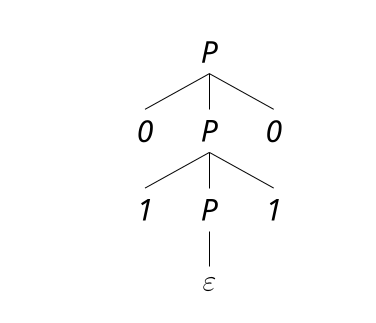
\includegraphics{example_1.1.1.png
}
%		\psframebox[linestyle=none,framesep=10pt]{%
%			\pstree{\LFTw{t}{\fontspec{Noto Sans}[Script=Latin]P}}{\pstree{\Tp[edge=none]}{%
%					\LFTw{t}{\fontspec{Noto Sans}[Script=Latin]0}
%					\pstree{\LFTw{t}{\fontspec{Noto Sans}[Script=Latin]P}}{\pstree{\Tp[edge=none]}{%
%							\LFTw{t}{\fontspec{Noto Sans}[Script=Latin]1}
%							\pstree{\LFTw{t}{\fontspec{Noto Sans}[Script=Latin]P}}{\pstree{\Tp[edge=none]}{%
%									\LFTw{t}{\fontspec{Noto Sans}[Script=Latin]$\varepsilon$}}}
%							\LFTw{t}{\fontspec{Noto Sans}[Script=Latin]1}}}
%					\LFTw{t}{\fontspec{Noto Sans}[Script=Latin]0}}}}
	\end{center}
\end{example}
\begin{example}
	Si ha:
	$$E\to I|\, E+E|\, E*E|\, (E)$$
	$$I\to a|\,b|\,Ia|\,Ib|\,I0|\,I1$$
	un albero sintattico per $a*(a+b00)$ può essere:
	\begin{center}
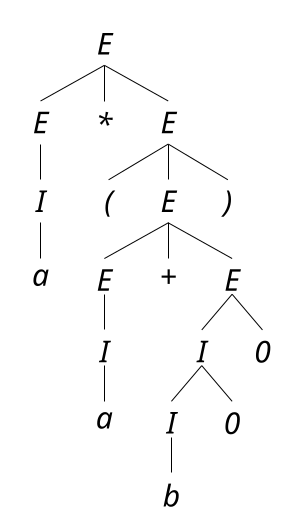
\includegraphics{example_1.1.2.png}
%		\psframebox[linestyle=none,framesep=10pt]{%
%			\pstree{\LFTw{t}{\fontspec{Noto Sans}[Script=Latin]E}}{\pstree{\Tp[edge=none]}{%
%					\pstree{\LFTw{t}{\fontspec{Noto Sans}[Script=Latin]E}}{\pstree{\Tp[edge=none]}{%
%							\pstree{\LFTw{t}{\fontspec{Noto Sans}[Script=Latin]I}}{\pstree{\Tp[edge=none]}{%
%									\LFTw{t}{\fontspec{Noto Sans}[Script=Latin]a}}}}}
%					\LFTw{t}{\fontspec{Noto Sans}[Script=Latin]*}
%					\pstree{\LFTw{t}{\fontspec{Noto Sans}[Script=Latin]E}}{\pstree{\Tp[edge=none]}{%
%							\LFTw{t}{\fontspec{Noto Sans}[Script=Latin](}
%								\pstree{\LFTw{t}{\fontspec{Noto Sans}[Script=Latin]E}}{\pstree{\Tp[edge=none]}{%
%										\pstree{\LFTw{t}{\fontspec{Noto Sans}[Script=Latin]E}}{\pstree{\Tp[edge=none]}{%
%												\pstree{\LFTw{t}{\fontspec{Noto Sans}[Script=Latin]I}}{\pstree{\Tp[edge=none]}{%
%														\LFTw{t}{\fontspec{Noto Sans}[Script=Latin]a}}}}}
%										\LFTw{t}{\fontspec{Noto Sans}[Script=Latin]+}
%										\pstree{\LFTw{t}{\fontspec{Noto Sans}[Script=Latin]E}}{\pstree{\Tp[edge=none]}{%
%												\pstree{\LFTw{t}{\fontspec{Noto Sans}[Script=Latin]I}}{\pstree{\Tp[edge=none]}{%
%														\pstree{\LFTw{t}{\fontspec{Noto Sans}[Script=Latin]I}}{\pstree{\Tp[edge=none]}{%
%																\LFTw{t}{\fontspec{Noto Sans}[Script=Latin]b}}}
%														\LFTw{t}{\fontspec{Noto Sans}[Script=Latin]0}}}
%												\LFTw{t}{\fontspec{Noto Sans}[Script=Latin]0}}}}}
%								\LFTw{t}{\fontspec{Noto Sans}[Script=Latin])}}}}}}
	\end{center}
\end{example}
\newpage
Data una CFG si ha che i seguenti cinque enunciati si equivalgono:
\begin{enumerate}
	\item la procedura di inferenza ricorsiva stailisce che una stringa $w$ di simboli terminali appartiene al linguaggio $L(A)$ con $A$ variabile
	\item $A\to ^*w$
	\item $A\to^*_{lm}w$
	\item $A\to^*_{rm}w$
	\item esiste un albero sintattico con radice $A$ e prodotto $w$
\end{enumerate}
queste 5 proposizioni si implicano l'uni l'altra:
\begin{center}
	\begin{tikzpicture}
		\node (top) at (0,0) {5};
		\node (a) at(-1,-0.5) {3};
		\node (b) at(0,-1) {4};
		\node (c) at(-2.0,-1.85) {2};
		\node (d) at(1.5,-2) {1};
		\draw [->] (top) -- (a);
		\draw [->] (top) -- (b);
		\draw [->] (a) -- (c);
		\draw [->] (b) -- (c);
		\draw [->] (c) -- (d);
		\draw [->] (d) -- (top);
	\end{tikzpicture}
\end{center}
vediamo qualche dimostrazione di implicazione tra queste proposizioni:
\begin{proof}[da 1 a 5]
	si procede per induzione:
	\begin{itemize}
		\item \textbf{caso base:} ho un livello solo (una sola riga), $\exists A\to w$:
					$$\overset{A}{\overset{\triangle}w}$$
		\item \textbf{caso passo:} suppongo vero per un numero di righe $\leq n$, lo dimsotro per $n+1$ righe:
					$$A\to X_1,X_2,...,X_k$$
					$$w=w_1,w_2,...,w_k$$
					ovvero, in meno di $n+1$ livelli:
					\begin{center}
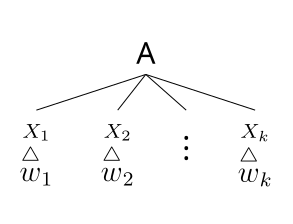
\includegraphics{caso_passo.png}
					% \psframebox[linestyle=none,framesep=10pt]{%
%				      \pstree{\LFTw{t}{\fontspec{Noto Sans}[Script=Latin]A}}{\pstree{\Tp[edge=none]}{%
%						      \LFTw{t}{\fontspec{Noto Sans}[Script=Latin]$\overset{X_1}{\overset{\triangle}w_1}$}
%						      \LFTw{t}{\fontspec{Noto Sans}[Script=Latin]$\overset{X_2}{\overset{\triangle}w_2}$}
%						      \LFTw{t}{\fontspec{Noto Sans}[Script=Latin]$\vdots$}
%						      \LFTw{t}{\fontspec{Noto Sans}[Script=Latin]$\overset{X_k}{\overset{\triangle}w_k}$}}}}
					\end{center}
	\end{itemize}
\end{proof}
\begin{proof}[da 5 a 3]
	procedo per induzione:
	\begin{itemize}
		\item \textbf{caso base (n=1): }$\exists A\to w\mbox{ quindi } A\to_{lm}w$, come prima si ha un solo livello:
					$$\overset{A}{\overset{\triangle}w}$$
		\item \textbf{caso passo: }suppongo che la proprierà valga per ogni albero di profondità minore uguale a $n$, dimostro che valga per gli alberi profondi $n+1$:
					$$A\to X_1,X_2,...,X_k$$
					$$w=w_1,w_2,...,w_k$$
					ovvero, in meno di $n+1$ livelli:
					\begin{center}
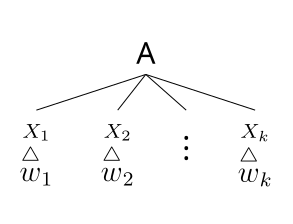
\includegraphics{caso_passo.png}
%			      \psframebox[linestyle=none,framesep=10pt]{%
%				      \pstree{\LFTw{t}{\fontspec{Noto Sans}[Script=Latin]A}}{\pstree{\Tp[edge=none]}{%
%						      \LFTw{t}{\fontspec{Noto Sans}[Script=Latin]$\overset{X_1}{\overset{\triangle}w_1}$}
%						      \LFTw{t}{\fontspec{Noto Sans}[Script=Latin]$\overset{X_2}{\overset{\triangle}w_2}$}
%						      \LFTw{t}{\fontspec{Noto Sans}[Script=Latin]$\vdots$}
%						      \LFTw{t}{\fontspec{Noto Sans}[Script=Latin]$\overset{X_k}{\overset{\triangle}w_k}$}}}}
					\end{center}
					$$A\to_{lm} X_1,X_2,...,X_k$$
					$$x_1\to^*_{lm}w_1 \mbox{ per ipotesi induttiva si ha un albero al più di n livelli}$$
					quindi:
					$$A\to_{lm}X_1,...,X_k\to^*_{lm}w_1,X_2,...,X_k\to^*_{lm}...\to^*_{lm}w_1,...,w_k=w$$
	\end{itemize}
	\begin{example}
		$$E\to I\to Ib\to ab$$
		$$\alpha E\beta\to\alpha I\beta\to \alpha Ib\beta\to \alpha ab\beta,\,\,\,\alpha,\beta\in(V\cup T)^*$$
	\end{example}
\end{proof}
\begin{example}
	Mostro l'esistenza di una derivazione sinistra dell'albero sintattico di $a*(a+b00)$:
	$$E\to^*_{lm}E*E\to^*_{lm}I*E\to^*_{lm}a*E\to^*_{lm}a*(E)\to^*_{lm}a*(E+E)\to^*_{lm}$$
	$$a*(I+E)\to^*_{lm}a*(a+E)\to^*_{lm}a*(a+I)\to^*_{lm}a+(a+I0)\to^*_{lm}a*(a+I00)\to^*_{lm}a*(a+b00)$$
\end{example}
\section{Grammatiche ambigue}
\begin{definition}
	Una grammatica è definita ambigua se esiste una stringa $w$ di terminali che ha più di un albero sintattico
\end{definition}
\begin{example}
	vediamo un esempio:
	\begin{enumerate}
		\item $E\to E+E\to E+E*E$
					ovvero:
					\begin{center}
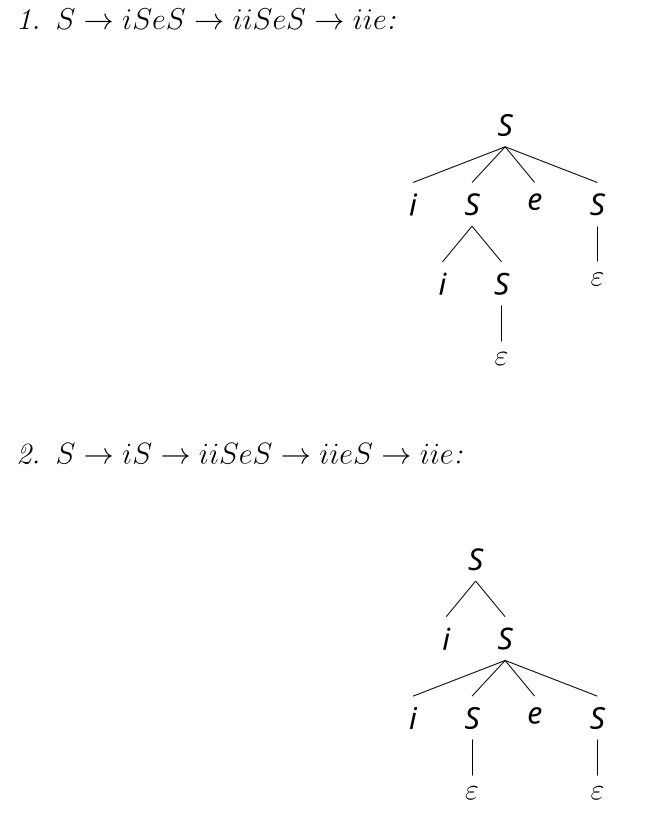
\includegraphics{ambigua1.png}
%			      \psframebox[linestyle=none,framesep=10pt]{%
%				      \pstree{\LFTw{t}{\fontspec{Noto Sans}[Script=Latin]E}}{\pstree{\Tp[edge=none]}{%
%						      \LFTw{t}{\fontspec{Noto Sans}[Script=Latin]E}
%						      \LFTw{t}{\fontspec{Noto Sans}[Script=Latin]+}
%						      \pstree{\LFTw{t}{\fontspec{Noto Sans}[Script=Latin]E}}{\pstree{\Tp[edge=none]}{%
%								      \LFTw{t}{\fontspec{Noto Sans}[Script=Latin]E}
%								      \LFTw{t}{\fontspec{Noto Sans}[Script=Latin]*}
%								      \LFTw{t}{\fontspec{Noto Sans}[Script=Latin]E}}}}}}
					\end{center}
		\item $E\to E*E\to E+E*E$
					ovvero:
					\begin{center}
%			      \psframebox[linestyle=none,framesep=10pt]{%
%				      \pstree{\LFTw{t}{\fontspec{Noto Sans}[Script=Latin]E}}{\pstree{\Tp[edge=none]}{%
%						      \pstree{\LFTw{t}{\fontspec{Noto Sans}[Script=Latin]E}}{\pstree{\Tp[edge=none]}{%
%								      \LFTw{t}{\fontspec{Noto Sans}[Script=Latin]E}
%								      \LFTw{t}{\fontspec{Noto Sans}[Script=Latin]+}
%								      \LFTw{t}{\fontspec{Noto Sans}[Script=Latin]E}}}
%						      \LFTw{t}{\fontspec{Noto Sans}[Script=Latin]*}
%						      \LFTw{t}{\fontspec{Noto Sans}[Script=Latin]E}}}}
					\end{center}
	\end{enumerate}
	si arriva a due stringhe uguali ma con alberi diversi. Introduciamo delle categorie sintatiche, dei vincoli alla produzione delle regole:
	\begin{enumerate}
		\item $E\to T|\, E+T$
		\item $T\to F|\, T+F$
		\item $F\to I|\, (E)$
		\item $I\to a|\,b|\,Ia|,Ib|\,I0|\,I1$
	\end{enumerate}
\end{example}
Possono esserci più derivazioni di una stringa ma l'importante è che non ci siano alberi sintattici diversi. Capire se una CFG è ambigua è un problema indecidibile
\begin{example}
	vediamo un esempio:
	$$S\to \varepsilon|\,SS|\, iS|\, iSeS$$
	con S=statement, i=if e e=else. Considero due derivazioni:
	\begin{enumerate}
		\item $S\to iSeS\to iiSeS\to iie$:
					\begin{center}
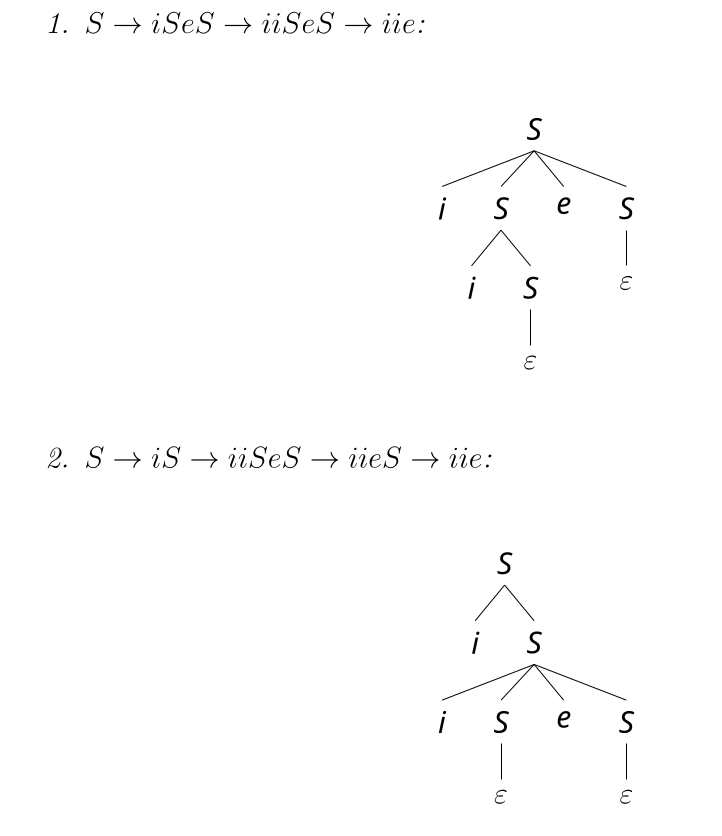
\includegraphics{ambigua2.png}

%			      \psframebox[linestyle=none,framesep=10pt]{%
%				      \pstree{\LFTw{t}{\fontspec{Noto Sans}[Script=Latin]S}}{\pstree{\Tp[edge=none]}{%
%						      \LFTw{t}{\fontspec{Noto Sans}[Script=Latin]i}
%						      \pstree{\LFTw{t}{\fontspec{Noto Sans}[Script=Latin]S}}{\pstree{\Tp[edge=none]}{%
%								      \LFTw{t}{\fontspec{Noto Sans}[Script=Latin]i}
%								      \pstree{\LFTw{t}{\fontspec{Noto Sans}[Script=Latin]S}}{\pstree{\Tp[edge=none]}{%
%										      \LFTw{t}{\fontspec{Noto Sans}[Script=Latin]$\varepsilon$}}}}}
%						      \LFTw{t}{\fontspec{Noto Sans}[Script=Latin]e}
%						      \pstree{\LFTw{t}{\fontspec{Noto Sans}[Script=Latin]S}}{\pstree{\Tp[edge=none]}{%
%								      \LFTw{t}{\fontspec{Noto Sans}[Script=Latin]$\varepsilon$}}}}}}\end{center}
%		\item $S\to iS\to iiSeS\to iieS\to iie$:
%		      \begin{center}
%
%			      \psframebox[linestyle=none,framesep=10pt]{%
%				      \pstree{\LFTw{t}{\fontspec{Noto Sans}[Script=Latin]S}}{\pstree{\Tp[edge=none]}{%
%						      \LFTw{t}{\fontspec{Noto Sans}[Script=Latin]i}
%						      \pstree{\LFTw{t}{\fontspec{Noto Sans}[Script=Latin]S}}{\pstree{\Tp[edge=none]}{%
%								      \LFTw{t}{\fontspec{Noto Sans}[Script=Latin]i}
%								      \pstree{\LFTw{t}{\fontspec{Noto Sans}[Script=Latin]S}}{\pstree{\Tp[edge=none]}{%
%										      \LFTw{t}{\fontspec{Noto Sans}[Script=Latin]$\varepsilon$}}}
%								      \LFTw{t}{\fontspec{Noto Sans}[Script=Latin]e}
%								      \pstree{\LFTw{t}{\fontspec{Noto Sans}[Script=Latin]S}}{\pstree{\Tp[edge=none]}{%
%										      \LFTw{t}{\fontspec{Noto Sans}[Script=Latin]$\varepsilon$}}}}}}}}
					\end{center}
	\end{enumerate}
	Si ha quindi una grammatica ambigua
\end{example}
\begin{theorem}
	Per ogni CFG, con $G=(V, T, P, S)$, per ogni stringa $w$ di terminali si ha che $w$ ha due alberi sintattici distinti sse ha due derivazioni sinistre da S distinte.\\
	Se la grammatica non è ambigua allora esiste un'unica derivazione sinistra da $S$
\end{theorem}
\subsubsection{Linguaggi inerentemente ambigui}
\begin{definition}
	Un linguaggio $L$ è inerentemente ambiguo se tutte le grammatiche CFG per tale linguaggio sono a loro volta ambigue
\end{definition}
\begin{example}
	Sia $L=\{a^nb^nc^md^m|\, n,m\geq 1\}\cup \{a^nbmnc^md^n|\, n,m\geq 1\}$\\
	si ha quindi un CFL formato dall'unione di due CFL. $L$ è inerentemente ambiguo e generato dalla seguente grammatica:
	\begin{itemize}
		\item $S\to AB|\,C$
		\item $A\to aAb|\,ab$
		\item $B\to cBd|\, cd$
		\item $C\to aCd|\, aDd$
		\item $D\to bDc|\, bc$
	\end{itemize}
	si possono avere due derivazioni:
	\begin{enumerate}
		\item $S\to_{lm}AB\to_{lm} aAbB\to_{lm} aabbB\to_{lm}aabbcBd\to_{lm}aabbccdd$
		\item $S\to_{lm} C\to_{lm} aCd\to_{lm}aaBdd\to_{lm}aabBcdd\to_{lm}aabbccdd$
	\end{enumerate}
	a generare problemi sono le stringhe con n=m perché possono essere prodotte in due modi diversi da entrambi i sottolinguaggi. Dato che l'intersezione tra i due sottolinguaggi non è buota si ha che $L$ è ambiguo
\end{example}
\section{Grammatiche Regolari}
Sono le grammatiche che generano i linguaggi regolari (quelli del terzo tipo) che sono casi particolari dei CFL.\\
Si ha la solita grammatica $G = (V, T, P, S)$ con però vincoli su $P$:
\begin{itemize}
	\item $\varepsilon$ si può ottenere solo con $S\to \varepsilon$
	\item le produzioni sono tutte lineari a destra ($A\to aA$ o $A\to a$) o a sinistra ($A\to Ba$ o $A\to a$)
\end{itemize}
\begin{example}
	$I\to a|\,b|\,Ia|\,Ib|\,I0|\,I1$ è una grammatica con le produzioni lineari a sinistra.\\
	Potremmo pensarlo a destra $I\to a|\,b|\,aI|\,bI|\,0I|\,1I$.\\
	Vediamo esempi di produzione con queste grammatiche:
	\begin{itemize}
		\item con $I\to a|\,b|\,Ia|\,Ib|\,I0|\,I1$ possiamo derivare $ab01b0$:
					$$I\to I0\to Ib0\to I1b0\to I01b0\to Ib01b0\to ab01b0$$
		\item con $I\to a|\,b|\,aI|\,bI|\,0I|\,1I$ invece non riusciamo a generare nulla:
					$$I\to 0I\to 0a$$
	\end{itemize}
	definisco quindi un'altra grammatica (con una nuova categoria sintattica):
	$$I\to aJ|\, bJ$$
	$$J\to a|\,b|\,aJ|\,bJ|\,0J|\,1J$$
	che però non mi permette di terminare le stringhe con 0 e 1, la modifico ancora otterdendo:
	$$I\to aJ|\, bJ$$
	$$J\to a|\,b|\,aJ|\,bJ|\,0J|\,1J|\,0|\,1$$
	e questo è il modo corretto per passare da lineare sinistra a lineare destra
\end{example}
\begin{example}
	Sia $G=(\{S\},\{0,1\},P,S)$ con $S\to \varepsilon|\,0|\,1|\,0S|\,1S$. Si ha quindi:
	$$L(G)=\{0,1\}^*$$
	si hanno comunque due proposizioni ridondanti, riducendo trovo:
	$$S\to \varepsilon|\, 0S|\,1S$$
	con solo produzioni lineari a destra. Con produzioni lineari a sinistra ottengo:
	$$S\to \varepsilon|\, S0|\,S1$$
\end{example}
\begin{example}
	Trovo una grammatica lineare destra e una sinistra per $L=\{a^nb^m|\,n,m\geq 0\}$:
	\begin{itemize}
		\item \textbf{lineare a destra:} si ha $G=(\{S,B\},\{a,b\},P,S)$ e quindi:
					$$S\to \varepsilon|\,aS|\,bB$$
					$$B\to bB|\,b$$
					ma non si possono generare stringhe di sole $b$, infatti:
					$$S\to aS\to abB\to abbB\to abbb$$
					ma aggiungere $\varepsilon$ a B \textbf{non è lecito}. posso però produrre la stessa stringa da due derivazioni diverse:
					$$S\to \varepsilon|\,aS|\,bB|\,b$$
					$$B\to bB|\,b$$
					che risulta quindi la nostra lineare a destra
		\item \textbf{lineare a sinistra:} si ha $G=(\{S,A\},\{a,b\},P,S)$ e quindi:
					$$S\to \varepsilon|\,Sb|\,Ab|\,a$$
					$$A\to Aa|\,a$$
	\end{itemize}
\end{example}
\begin{example}
	Trovo una grammatica lineare destra e una sinistra per $L=\{ab^ncd^me|\,n\geq 0\,,m> 0\}$:
	\begin{itemize}
		\item \textbf{lineare a destra:} si ha  si ha $G=(\{S,A,B,E\},\{a,b,c,d,e\},P,S)$ e quindi:
					$$S\to aA$$
					$$A\to bA|\,cB$$
					$$B\to dB|\, dE$$
					$$E\to e$$
		\item \textbf{lineare a sinistra:} si ha  si ha $G=(\{S,X,Y,Z\},\{a,b,c,d,e\},P,S)$ e quindi:
					$$S\to Xe$$
					$$A\to Xd|\,Yd$$
					$$B\to Zc$$
					$$E\to a|\,Zb$$
	\end{itemize}
	quindi se per esempio ho la stringa "ciao" si ha:
	\begin{itemize}
		\item \textbf{lineare a destra:}
					$$S\to Ao$$
					$$A\to Ba$$
					$$B\to Ei$$
					$$E\to c$$
		\item \textbf{lineare a sinistra:}
					$$S\to cA$$
					$$A\to iB$$
					$$B\to aE$$
					$$E\to o$$
	\end{itemize}
\end{example}
\begin{example}
	A partire da $G=(\{S,T\},\{0,1\},P,S)$ con:
	$$S\to\varepsilon|\,0S|\,1T$$
	$$T\to 0T|\,1S$$

	trovo come è fatto $L(G)$:
	$$L(G)=\{w\in\{0,1\}^*|\, w \mbox{ ha un numero di 1 pari}\}$$
\end{example}
\begin{example}
	fornire una grammatica regolare a destra e sinistra per:
	$$L=\{w\in\{0,1\}^*|\, w \mbox{ ha almeno uno 0 o almeno un 1}\}$$
	Si ah che tutte le stringhe tranne quella vuota ciontengono uno 0 o un 1
	quindi  $G=(\{S\},\{0,1\},P,S)$:
	\begin{itemize}
		\item \textbf{lineare a destra:}
					$$S\to 0|\,1|\,0S|\,1S$$
		\item \textbf{lineare a sinistra:}
					$$S\to 0|\,1|\,S0|\,S1$$
	\end{itemize}
\end{example}



Vediamo ora un esempio di \textit{Context Free Language (CFL)}, costruito a partire da una \textit{Context Free Grammar (CFG)}:
\begin{example}
	Sia $\Sigma=\{0, 1\}$ e $L_{pal}="stringhe\,\, palindrome\,\, binarie"$.
	Quindi, per esempio, $0110\in L,\,\, 11011\in L$ ma $10010\not\in L$. Si ha che $\varepsilon$, la stringa vuota, appartiene a $L$. Diamo una definizione ricorsiva:
	\begin{itemize}
		\item \textbf{base:} $\varepsilon,\, 0\,\ 1\in L_{pal}$
		\item \textbf{passo:} se $w$ è palindroma allora $0w0$ è palindromo e $1w1$ è palindromo
	\end{itemize}
	una variabile generica $S$ può sottostare alle \textit{regole di produzione} di una certa grammatica. In questo caso si ha uno dei seguenti:
	$$S\to\varepsilon,\, S\to 0,\, S\to 1,\, S\to 0S0,\, S\to 1S1$$
\end{example}


riprendiamo l'esempio sopra:
\begin{example}
	$$G_{pal}=(V=\{S\},\, T=\{0, 1\},\, P,\, S)$$
	con:
	$$P=\{S\to\varepsilon,\, S\to 0,\, S\to 1,\, S\to 0S0,\, S\to 1S1\}$$
	Si può ora costruire un algoritmo per creare una stringa palindroma a partire dalla grammatica $G$:
	$$\underbrace{S}_{\mbox{start}}\underbrace{\to}_{\mbox{applico una regola}} 1S1 \to 01S10\to \underbrace{01010}_{\mbox{sostituisco variabile}}$$

	con $S,\, 1S1\,\, e\,\, 01S10$ che sono \textit{forme sentenziali}. Posso così ottenere tutte le possibili stringhe. Esiste anche una forma abbreviata:
	$$S\to \varepsilon|o|1|0S0|1S1$$
	Non si fanno sostituzioni in parallelo, prima una $S$ e poi un'altra
\end{example}

%%% Local Variables:
%%% mode: LaTeX
%%% TeX-master: "../libro-linguaggi"
%%% TeX-engine: luatex
%%% End:

%\setchapterpreamble[u]{\margintoc}
\chapter{Linguaggi Regolari}\label{cha:Linguaggi-regolari}




\section{Introduzione}\label{sec:regolari-introduzione}

In questo caso vogliamo identificare una classe di linguaggi che sia semplice da definire, che ammetta un riconoscitore
efficiente, ma non sia così ristretta da ammettere solo linguaggi banali.
Per ottenere questo obiettivo, introduciamo le espressioni regolari che portano ad una definizione di tipo
insiemistico dei linguaggi regolari.

\begin{definition}[espressione regolare]\label{def:regex}
Sia $\Sigma$ un alfabeto. Un'\keyword{espressione regolare} è definita secondo le seguenti regole.
\begin{enumerate}
\item $\varepsilon$ e $\emptyset$ sono espressioni regolari;
\item Ogni simbolo $\sigma\in\Sigma$ è un'espressione regolare;
\item Se $E_1$ e $E_2$ sono due espressioni regolari, allora $E_1 \cup E_2$ è un'espressione regolare corrispondente
	  all'unione, o alternanza, fra $E_1$ e $E_2$;
\item Se $E_1$ e $E_2$ sono due espressioni regolari, allora $E_1 E_2$ è un'espressione regolare corrispondente
	  alla concatenazione di $E_1$ e $E_2$;
\item Se $E$ è un'espressione regolare, allora $E_1^{*}$ è un'espressione regolare corrispondente
	  alla chiusura di Kleene di $E$, ovvero alla ripetizione di $E$ un numero imprecisato (incluso $0$) di volte;
\item Se $E$ è un'espressione regolare, allora $(E)$ è un'espressione regolare.
\end{enumerate}
\end{definition}

Le operazioni hanno un ordine di precedenza di valutazione (a parità di precedenza, si valuta da sinistra a destra), in
ordine descrescente di precedenza:
\begin{enumerate}
	\item parentesi
	\item chiusura di Kleene *
	\item concatenazione
	\item unione
\end{enumerate}


Notiamo che le espressioni regolari sono una sintassi che, al momento, può apparire priva di significato concreto.
Abbiamo bisogno di introdurre il linguaggio associato ad un'espressione regolare, seguendo pedissequamente i casi della \Cref{def:regex}.

\begin{definition}[Linguaggio associato ad un'espressione regolare]\label{def:regex-linguaggio}
Sia $E$ un'espressione regolare. Il linguaggio $L(E)$ associato a $E$ è definito secondo le seguenti regole.
\begin{enumerate}
	  \item $L(\epsilon) = \{\epsilon\}$, $L(\emptyset) = \emptyset$;
\item Se $E$ consiste unicamente di un simbolo $\sigma\in\Sigma$, allora $L(E) = \{\sigma\}$;
\item Se $E=E_1 \cup E_2$, allora $L(E) = \{w\in \Sigma^{*} : w\in L(E_{1}) \vee  w\in L(E_{2})\}$;
\item Se $E=E_1E_2$, allora $L(E) = \{ w_{1}w_{2} : w\in L(E_1) L(E_2) \}$;
\item Se $E = E_1^{*}$, allora $L(E) = \{\epsilon\} \cup L(E_1) \bigcup_{k=1}^{*} \{w_1 \cdots w_{k}: w_{1}, \ldots, w_{k}\in L(E) \}$.
\item Se $E = (E_1)$, allora $L(((E)) = L(E)$.
\end{enumerate}
\end{definition}

Un linguaggio $L$ viene detto regolare se e solo se esiste un'espressione regolare $E$ che ha $L$ come linguaggio associato.
Notiamo che un'espressione regolare non è una grammatica, ma una sintassi minimale per specificare un linguaggio regolare.
Se consideriamo due espressioni regolari identiche quando hanno lo stesso linguaggio associato, possiamo dare alcune proprietà delle operazioni.

\begin{proposition}\label{prop:regex-associative-commutative}
\begin{itemize}
\item
L'unione è commutativa ($E_1 \cup E_2 = E_2 \cup E_1$), associativa $E_1 \cup (E_2 \cup E_3) = (E_1 \cup E_2) \cup E_3$
e idempotente ($E\cup E = E$).
\item
La concatenazione è associativa ma non è commutativa.
\item
	  $\emptyset$ è identità per l'unione ($\emptyset+E=E+\emptyset=E$),
\item
	  $ \{\varepsilon \} $ è identità per la concatenazione
($\varepsilon E=E\varepsilon=L$).
\item
$\emptyset$ è l'annichilitore per la concatenazione ($\emptyset L=L\emptyset=\emptyset$).
\item
	$(E^{*})^{*}=E^{*}$,
\item
$\emptyset^*=\varepsilon$;
\item
$\varepsilon^*=\varepsilon$;
\end{itemize}
\end{proposition}

L'enfasi sulla minimalità della sintassi è tipica dell'analisi della capacità espressiva.
In altre parole, per capire quali siano i linguaggi regolari è preferibile avere espressioni costruite a partire da un
numero estremamente limitato di operazioni.
Se invece vogliamo pensare ad espressioni regolari che possano essere utilizzate in pratica, ci aspettiamo di avere
altre operazioni o della sintassi addizionale che permetta di esprimere con semplicità casi particolarmente rilevanti.
Mostriamo di seguito alcune possibili estensioni della \Cref{def:regex} che \textbf{non ne aumentano il potere espressivo}.
In altre parole, l'insieme dei linguaggi associati ad un'espressione regolare non cambia se ammettiamo queste
estensioni, dove $E$, $E_1$, $E_2$ sono tutte espressioni regolari:

\begin{enumerate}
\item $E^{+}$, corrispondente  alla ripetizione di $E$ un numero imprecisato, ma strettamente positivo,  di volte.
È equivalente all'espressione $E E^{*}$;
\item $E\{n,m\}$, corrispondente  alla ripetizione di $E$ un numero di volte compreso fra $n$ ed $m$, estremi inclusi.
L'espressione $E\{0,0\}$ è equivalente a $\epsilon$, $E\{0,m\}$ (con $m>0$) è equivalente a $E \cup E\{1,m\}$,
	  $E\{n,m\}$ (con $n>0$) è equivalente a $E E\{n-1,m-1\}$;
\item $[abc]$, dove $a$, $b$, $c$ sono tutti simboli di $\Sigma$, corrisponde alla scelta fra i simboli indicati.
	  L'espressione regolare equivalente è $a\cup b\cup c$;
\item $[\^ abc]$, dove $a$, $b$, $c$ sono tutti simboli di $\Sigma$, corrisponde alla scelta fra i simboli \emph{non} indicati.
	  L'espressione regolare equivalente è $\bigcup_{a_{1}\in \Sigma \setminus \{a,b,c\}} a_{1}$.
\end{enumerate}



% le regex sono usate per la ricerca di un pattern in un testo o negli analizzatori lessicali. Una regex denota il linguaggio e non la grammatica. Si hanno le seguenti operazioni tra due linguaggi $L$ e $M$:
% \begin{itemize}
% 	\item \textbf{unione:} dati $L,\, M\in \Sigma^*$, l'unione $L\cup M$ è l'insieme delle stringhe che si trovano in entrambi i linguaggi o solo in uno dei due
% 				\begin{example}
% 					$$L=\{001,10,111\}$$
% 					$$M=\{\epsilon,001\}$$
% 					$$L\cup M=\{\epsilon,01,10,111,\epsilon\}$$
% 				\end{example}
% 				si ha che:
% 				$$L\cup M=M\cup L$$
% 	\item \textbf{concatenazione:} dati $L,\, M\in \Sigma^*$, la concatenazione $L\cdot M$ (o $LM$) è lisieme di tutte le stringhe ottenibili concatenandone una di $L$ a una di $M$
% 				\begin{example}
% 					$$L=\{001,10,111\}$$
% 					$$M=\{\epsilon,001\}$$
% 					$$L\cdot M=\{001,001001,10,\cdots\}$$
% 				\end{example}
% 				si ha che:
% 				$$L\cdot M\neq M\cdot L$$
% 	\item si definiscono:
% 				\begin{itemize}
% 					\item $L\cdot L=L^2$, $L\cdot L\cdot L=L^3$ etc\cdots
% 					\item $L^1=L$
% 					\item $L^0=\{\epsilon\}$
% 				\end{itemize}
% 	\item \textbf{chiusura di Kleene:} dato $L\subseteq \Sigma^*$ si ha che la chiusura di Kleen di $L$ è:
% 				$$L^*=\underset{i\geq 0}{\cup}L^i$$
% 				ricordando che $l^0=\epsilon$
% 				\begin{example}
% 					Sia $L=\{0,11\}$, si ha:
% 					$$L^0=\epsilon$$
% 					$$L^1=L=\{0,11\}$$
% 					$$L^2=L\cdot L=\{00,011,110,1111\}$$
% 					$$L^3=L\cdot L\cdot L=L^2\cdot L=\{000,0110,1100,11110,0011,01111,11011,111111\}$$
% 				\end{example}
% 				vediamo dei casi particolari:
% 				\begin{itemize}
% 					\item $L=\{0^n|\,n\geq 0\}$ implica $|L|=\infty$ e quindi, essendo $L^i=L,\, i\geq 1$ e quindi $|L^i|=\infty$, $|L^*|=\infty$. Si ha quindi:
% 								$$L^*=L^0\cup L^1\cup \cdots \cup L^i=L$$
% 					\item $L=\emptyset$ implica $L^0=\{\epsilon\}$, $L^2=L\cdot L=\emptyset$ e così via per ogni concatenazione di $L$. Si ha quindi:
% 								$$L^*=L^0=\{\epsilon\}$$
% 					\item $L=\{\epsilon\}$ implica $L^0=\{\epsilon\}=L=L^1=L^2=\cdots$, si ha quindi:
% 								$$L^*=\{\epsilon\}=L$$
% 				\end{itemize}
% 				L'insieme vuoto e l'insieme contenente la stringa vuota hanno le uniche chiusure di kleene finite
% \end{itemize}
% \begin{definition}
% 	Si riporta la definizione ricorsiva di un'espressione regolare:
% 	\begin{itemize}
% 		\item \textbf{casi base:} si hanno tre casi base:
% 					\begin{enumerate}
% 						\item $\epsilon$ e $\emptyset$ sono espressioni regolari
% 						\item se $a\in \Sigma$, con $a$ che è un'esprssione regolare, $L(a)=\{a\}$
% 						\item le variabili che rappresentano linguaggi regolari sono espressioni regolari, $L(L)=L$
% 					\end{enumerate}
% 		\item \textbf{casi passo:} si hanno i 4 casi passo:
% 					\begin{enumerate}
% 						\item \textbf{unione:} se $E$ e $F$ sono espressioni regolari allora anche $E+F=E\cup F$ è un'espressione regolare e si ha:
% 									$$L(E+F)=L(E)\cup L(F)$$
% 						\item \textbf{concatenazione:} se $E$ e $F$ sono espressioni regolari allora anche $EF=E\cdot F$ è un'espressione regolare e si ha:
% 									$$L(EF)=L(E)\cdot L(F)$$
% 						\item \textbf{chiusura:} se $E$ è un'espressione regolare allora $E^*$ è un'espressione regolare e si ha:
% 									$$L(E^*)=(L(E))^*$$
% 						\item \textbf{parentesi:} se $E$è un'espressione regolare allora $(E)$ è un'espressione regolare e si ha:
% 									$$L((E))=L(E)$$
% 					\end{enumerate}
% 	\end{itemize}
% 	\newpage

L'idea di estendere un modello con nuove operazioni che non ne aumentano il potere espressivo semplifica notevolmente lo
studio di tale potere espressivo.
Intuitivamente, consideriamo due modelli $M_{1}$ e $M_2$, entrambi dotati di un insieme ridotto di operazioni.
Sia $M_1$ che $M_2$ vengono estesi (ottenendo rispettivamente i modelli estesi $M_1^{*}$ e $M_2^{*}$) senza aumentare il
rispettivo potere espressivo.
Quando vogliamo dimostrare che i due modelli $M_1$ e $M_2$ hanno lo stesso potere espressivo, possiamo simulare $M_1$
con $M_2^{*}$ (mostrando quindi che tutto quello che può essere fatto con $M_1$ può essere fatto con $M_2^{*}$) e
simulare $M_2$ con $M_1^{*}$.
In questo caso, il fatto di potere usare due modelli estesi rende più semplice la dimostrazione di correttezza della simulazione.
Al tempo stesso, studiare un modello ristretto, come $M_1$, rende più semplice dimostrare che qualcosa \emph{non} può
essere realizzato da $M_1$.
Sfrutteremo questa intuizione nel resto del libro.


\begin{example}\label{exa:01}
Si consideri il linguaggio su $\Sigma_{B}$ delle parole non nulle formate da  \texttt{0} e \texttt{1} alternati --- equivalentemente, nessuna
parola contiene la sottostringa  \texttt{00} e \texttt{11} ---
Trovare un'espressione regolare che ha associato tale linguaggio.

Dividiamo le parole del linguaggio a seconda che abbiano lunghezza pari o dispari e che inizino per \texttt{0} e
\texttt{1}, facendo l'unione di questi quattro linguaggi.
Otteniamo così l'espressione $(\mathtt{01})^* | (\mathtt{10})^* | \mathtt{1}(\mathtt{01})^* | \mathtt{0}(\mathtt{10})^*$.

		\[01\to \{01\}\]
		$$(01)^*\to \{\epsilon, 01, 0101,010101,\cdots\}$$
		$$(01)^{*} + (10)^{*} \to \{ \epsilon, 01,10,0101,1010, \cdots \} $$
		ma posso volere diverse quantità di 0 e 1, sempre mantenendo l'alternanza, metto o uno 0 o un 1 davanti a quanto ottenuto appena sopra:
		$$(01)^*+(10)^*+0(10)^*+1(01)^*\to \{\epsilon,01,10,010,101,\cdots\}$$
		non è comunque l'unica soluzione, si può avere:
		$$(\epsilon+1)(01)^*(\epsilon+0)\to \{\epsilon,01,10,010,101,\cdots\}$$
		oppure ancora:
		$$(\epsilon+0)(10)^*(\epsilon+1)$$
\end{example}


\begin{Exercise}[label=3-1]
Ho $E=(0+1)^*0^*(01)^*$:
\begin{itemize}
\item 001 fa parte del linguaggio?
\item 1001 fa parte del linguaggio?
\item 0101 fa parte del linguaggio?
\item 0 fa parte del linguaggio?
\item 10 fa parte del linguaggio?
\end{itemize}
\end{Exercise}


\begin{Answer}
\begin{itemize}
\item 001 è una parola del linguaggio: $\epsilon\cdot 0\cdot 01$
\item 1001 è una parola del linguaggio: $1\cdot 0\cdot 01$
\item 0101 è una parola del linguaggio: $\epsilon\cdot\epsilon \cdot 0101$
\item 0 è una parola del linguaggio: $\epsilon\cdot 0\cdot \epsilon$
\item 10 è una parola del linguaggio: $1\cdot 0\cdot \epsilon$
\end{itemize}



Notare che in realtà $L((0+1)^*)= \Sigma_{B}^*$ e le parti che seguono sono opzionali (la chiusura di Kleene permette di
avere la stringa vuota).
Quindi il linguaggio associato all'espressione regolare è $\Sigma_{B}^*$.
\end{Answer}

Si ricorda che:
$(0+1)^*\neq 0^*+1^*$

\begin{example}
	ho $ER=((01)^*\cdot 10\cdot (0+1)^*)^*$
	\begin{itemize}
		\item 0101 fa parte del linguaggio? No
		\item 01000 fa parte del linguaggio? No
		\item 01011 fa parte del linguaggio? No
		\item 10111 fa parte del linguaggio? Si, $\epsilon\cdot 10\cdot 111$
		\item 101010 fa parte del linguaggio? Si, prendo $10\cdot 1010$
		\item 101101 fa parte del linguaggio? Si, $\epsilon\cdot 10\cdot 1$ due volte
		\item 0101100011 fa parte del linguaggio? Si, $0101\cdot 10\cdot 0011$ (0011 lo posso prendere da $(0+1)^*$)
	\end{itemize}
\end{example}
\begin{example}
ho $ER=((01)^*\cdot 10\cdot (0+1))^*$
\begin{itemize}
		\item 0101 fa parte del linguaggio? No
		\item 01000 fa parte del linguaggio? No
		\item 01011 fa parte del linguaggio? No
		\item 10111 fa parte del linguaggio? No
		\item 101010 fa parte del linguaggio? No
		\item 101101 fa parte del linguaggio? Si, $\epsilon\cdot 10\cdot 1$ due volte
		\item 0101100011 fa parte del linguaggio? No
	\end{itemize}
\end{example}
\begin{example}
	Da $L\subseteq\{0,1\}|\mbox{ stringhe contenenti almeno una volta 01}$
	quindi:
	$(0+1)^*01(0+1)^*$
\end{example}
\begin{example}
	ho $ER=(00^*1^*)^*$, quindi:
	$L=\{\epsilon,0,01,000,001,010,011\}=\{\epsilon\}\cup\{ w\in \{0,1\}^* |\text{ w che inizia con 0}\}$
\end{example}

\begin{example}
	ho $ER=a(a+b)^*b$, quindi:
	$L=\{w\in\{a,b\}^*|\text{ w inizia con a e termina con b}\}$
\end{example}

\begin{example}
	ho $ER=(0^*1^*)^*000(0+1)^*$, quindi, sapendo che $\{0,1\}^*$ mi permette tutte le combinazioni che voglio come $(0+1)^*$:
	$L=\{w\in\{0,1\}^*|\text{ w come voglio con tre 0 consecutivi}\}$
\end{example}
\begin{example}
	ho $ER=a(a+b)^*c(a+b)^*c(a+b)^*b$, quindi:
	$L=\{w\in\{a,b,c\}^*|\text{ w inizia con a, termina con b  e contiene almeno due c, }$
	$\text{eventualmente non adiacenti}\}$
\end{example}
\begin{example}
Da $L\subseteq\{0,1\}$
 ogni 1 è seguito da 0, a meno che non sia l'ultimo carattere, ovvero 11 non compare

	quindi:
	$(10+0)^*(\epsilon+1)^*$
\end{example}
\begin{example}
	cerco ER per $L\subseteq\{0,1\}^*|\, \text{stringhe contenenti un numero pari di 1}$:
	$(0^*10^*1)^*0^*$
	oppure:
	$(0+10^*1)^*$
\end{example}
\begin{example}
	cerco ER per $L\subseteq\{0,1\}^*|\, \text{stringhe contenenti un numero dispari di 1}$:
	$(0^*10^*)^*0^*10^*$
	oppure:
	$(0+10^*1)^*10^*$
\end{example}
\begin{example}
	cerco ER per $L\subseteq\{0,1\}^*|\, \text{stringhe contenenti un numero divisibile per 3 di 0}$:
	$(1^*01^*01^*0)^*1^*$
\end{example}
\begin{example}
	cerco ER per $L\subseteq\{0,1\}^*|\, \text{stringhe contenenti al più una coppia di 1 consecutivi}$:
	$(10+0)^*(11+1+\epsilon)(01+0)^*$
\end{example}
\begin{example}
	cerco ER per $L\subseteq\{a,b,c\}^*|\, \text{stringhe contenenti almeno una a e almeno una b}:$
	$c^*\left(a(a+c)^*b+b(b+c)^*a\right)(a+b+c)^*$
\end{example}

\begin{Exercise}[label=0e1-er]
Sia $L\subseteq \Sigma_{B}^{*}$ il linguaggio delle parole che contengono almeno un \uno e almeno uno \zero.
Descrivere un'espressione regolare associata al linguaggio $L$.
\end{Exercise}



\begin{Exercise}[label=re-crescente]
Sia $L\subseteq \Sigma_{C}^{*}$ il linguaggio delle parole in cui le cifre compaiono in ordine non decrescente (ad esempio
\texttt{001112}).
Descrivere un'espressione regolare associata al linguaggio $L$.
\end{Exercise}

\begin{Answer}
Siccome non è richiesto che ogni cifra in $\Sigma_{C}$ sia presente nella parola, un'espressione è $0^{*}1^{*}2^{*}3^{*}4^{*}5^{*}6^{*}7^{*}8^{*}9^{*}$.
\end{Answer}


\begin{Exercise}[label=re-1-101]
Sia $L\subseteq \Sigma_{B}^{*}$ il linguaggio delle parole in cui compare esattamente una volta la sottostringa
\texttt{0110101}).
Descrivere un'espressione regolare associata al linguaggio $L$.
\end{Exercise}

\begin{Answer}
La difficoltà principale dell'esercizio consiste nello scrivere un'espressione regolare corrispondente a tutte le
stringhe binarie che non contengono \texttt{0110101}.
Un'espressione di questo tipo è
\end{Answer}

\begin{Exercise}[label=re-2-101]
Sia $L\subseteq \Sigma_{B}^{*}$ il linguaggio delle parole in cui compare esattamente due volte la sottostringa
\texttt{0110101}).
Descrivere un'espressione regolare associata al linguaggio $L$.
\end{Exercise}

\begin{Exercise}[label=re-2-11]
Sia $L\subseteq \Sigma_{B}^{*}$ il linguaggio delle parole in cui compare esattamente due volte la sottostringa
\texttt{11}).
Descrivere un'espressione regolare associata al linguaggio $L$.
\end{Exercise}


\section{Grammatiche regolari}\label{sec:grammatiche-regolari}

Una grammatica è regolare se ha una delle seguenti due forme.


\begin{definition}\label{def:grammatica-regolare-destra}
Sia \gramm una grammatica.
Allora $G$ è detta regolare destra se tutte le su produzioni sono nella forma $A \to a$ o nella forma $A \to Ba$, dove
$A, \in VB$  e $a\in T$.
Inoltre, $G$ è detta regolare sinistra se tutte le su produzioni sono nella forma $A \to a$ o nella forma $A \to aB$, dove
$A, \in VB$  e $a\in T$.
\end{definition}


\section{Diagrammi di transizione}\label{sec:diagrammi-di-transizione}

Consideriamo il diagramma di \Cref{fig:diagramma-transizione}, dove i nodi sono degli stati e le frecce rappresentano
transizioni fra stati al verificarsi di una determinata condizione.
Il diagramma rappresenta un tipico ciclo di edit, compilazione, test, messa in produzione del codice.
Questa idea può essere formalizzata in un modello di calcolo che è in grado di riconoscere i linguaggi regolari, come
vedremo nella prossima sezione.


\begin{figure}[ht!]
\includestandalone[width=\textwidth]{diagramma-transizione}
\caption{Esempio di diagramma di transizione}
\label{fig:diagramma-transizione}\end{figure}


\section{Automi deterministico a stati finiti}\label{sec:DFA}

L'obiettivo di questa sezione è introdurre un modello di calcolo, ispirato ai diagrammi di transizione, che sia il più
semplice possibile e in grado di riconoscere tutti i linguaggi regolari.
Questo modello viene chiamato automa a stati finiti deterministico (\keyword{DFA}).

\begin{definition}[automa deterministico a stati finiti]\label{def:DFA}
Un \keyword{automa deterministico a stati finiti} è una quintupla \dfa consiste nelle seguenti parti:
\begin{itemize}
	\item $\Sigma$: alfabeto di input;
	\item $Q$: insieme finito di \emph{stati};
	\item $\delta: Q\times \Sigma \mapsto Q$: \emph{funzione di transizione}.
Prende come argomento uno stato e un simbolo di input e restituisce uno stato;
	\item $q_{0}\in Q$: stato iniziale;
	\item $F\subseteq Q$: insieme di \emph{stati finali}, o accettanti.
\end{itemize}
\end{definition}

L'idea intuitiva è che iniziamo nello stato $q_{0}$.
Ad ogni passo viene letto (o \emph{consumato}) un carattere $c$ in input e determinato il prossimo stato tramite la
funzione di transizione.
Più precisamente, l'automa si muove nello stato $\delta(q,c)$, dove $q$ è lo stato attuale.
Dopo avere consumato tutta la stringa in input, questa stringa viene accettata (o riconosciuta) se e solo se l'automa si
trova in uno stato finale.
La \ref{def:DFA} specifica un automa \emph{deterministico} a stati finiti in quanto la funzione di transizione
restituisce esattamente un singolo stato e riceve esattamente un carattere.
Di conseguenza l'automa si trova sempre in un solo stato.

La descrizione della funzione di transizione $\delta$ può avvenire in due modi: con una tabella dove vengono indicati
tutti i valori di $\delta(q,c)$, oppure con un diagramma che ricorda quelli di transizione.
Nell'ultimo caso denotiamo lo stato iniziale con una freccia entrante che non ha un nodo di inizio, gli stati finali con
un doppio cerchio, e l'etichetta di un arco dallo stato $q_1$ allo stato $q_2$ è l'insieme di caratteri $c$ tali che
$\delta(q_1, c) = q_2 $.
\begin{example}
Consideriamo il linguaggio $L$ formato dalle strighe binarie che hanno la sottostringa \texttt{01}.
Equivalentemente $L=\{ x\mathtt{01}y: x,y \in \Sigma_{B}^{*}\}$.
Leggendo la stringa in input, l'automa è in uno dei seguenti casi:
	\begin{enumerate}
		\item se ha "già visto" 01, accetterà qualsiasi input, indipendentemente dai caratteri che leggerà in futuro;
		\item pur non avendo ancora visto 01, l'input più recente è stato 0.
Se leggerà \texttt{1}, andrà nello stato accettante, altrimenti rimane nello stesso stato;
		\item non ha ancora visto \texttt{0}, e rimane in questo stato finchè non legge \texttt{0}.
	\end{enumerate}
	la terza condizione rappresenta lo stato iniziale. All'inizio bisogna vedere uno 0 e poi un 1. Ma se nello stato $q_0$ si vede per primo un 1 allora non abbiamo fatto alcun passo verso 01, e dunque dobbiamo permanere nello stato $q_0$, $\delta(q_0,1)=q_0$. D'altra parte se nello stato iniziale vedo 0 siamo nella seconda condizione, uso quindi $q_2$ per questa condizione, si avrà quindi $\delta(q_0,0)=q_2$. Vedo ora le transizoni di $q_2$, se vedo 0 ho che 0 è l'ultimo simbolo incontrato quindi uso nuovamente $q_2$, $\delta(q_2,0)=q_2$, in attesa di un 1. Se arriva 1 passo allo stato accertante $q_1$ corrispondente alla prima condizione, $\delta(q_2,1)=q_1$. Ora abbiamo incontrato 01 quindi può succedere qualsiasi cosa e dopo qualsiasi cosa accada potremo nuovamente aspettarci qualsiasi cosa, ovvero $\delta(q_1,0)=\delta(q_1,1)=q_1$. Si deduce quindi che:
	$Q=\{q_0,q_1,q_2\} \text{ e } F=\{q_1\}$
	quindi:
	$A=\{\{q_0,q_1,q_2\} ,\{0,1\}, \delta, q_0, \{q_1\} \}$
	con in totale le seguenti transizioni:
	$\delta(q_0,1)=q_0$
	$\delta(q_0,0)=q_2$
	$\delta(q_2,0)=q_2$
	$\delta(q_2,1)=q_1$
	$\delta(q_1,0)=q_1$
	$\delta(q_1,1)=q_1$
\end{example}

\begin{margintable}
	\begin{center}
		\begin{tabular}{c|c|c}
			$\delta$   & 0     & 1     \\
			\hline
			$\to\,q_0$ & $q_1$ & $q_0$ \\
			\hline
			$*\,q_1$   & $q_1$ & $q_1$ \\
			\hline
			$q_2$      & $q_2$ & $q_1$
		\end{tabular}
	\end{center}
\caption{L'automa di \cref{fig:dfa-sottostringa-01}, in forma tabellare.}
\end{margintable}


\begin{figure}[ht!]
\includestandalone[width=\textwidth]{dfa-sottostringa-01}
\caption{DFA che accetta il linguaggio $\Sigma_{B}^{*}\mathtt{01}\Sigma_{B}^{*}$}
\label{fig:dfa-sottostringa-01}\end{figure}




\begin{example}
	Trovo automa per: $L=\{w\in\{a,b\}^*|\text{ w che contiene un numero pari di b}\}$
	\begin{center}
		\begin{tikzpicture}[shorten >=1pt,node distance=3cm,on grid,auto]
			\node[state, initial, accepting] (q_0) {$q_0$};
			\node[state] (q_1) [right=of q_0] {$q_1$};
			\path[->]
			(q_0) edge [bend left = 25] node {b} (q_1)
			edge [loop below] node {a} ()
			(q_1) edge [bend left = 25] node {b} (q_0)
			edge [loop below] node {a} ();
		\end{tikzpicture}
	\end{center}
	ovvero se da $q_0$ vado a $q_1$ sono obbligato ab generare due $b$, dato che il nodo accettnate è $q_0$. In entrambi i nodi posso generare quante $a$ voglio.
\end{example}
\begin{example}
	Trovo automa per: $L=\{w\in\{a,b\}^*|\text{ w che contiene un numero dispari di b}\}$
	\begin{center}
		\begin{tikzpicture}[shorten >=1pt,node distance=3cm,on grid,auto]
			\node[state, initial] (q_0) {$q_0$};
			\node[state, accepting] (q_1) [right=of q_0] {$q_1$};
			\path[->]
			(q_0) edge [bend left = 25] node {b} (q_1)
			edge [loop below] node {a} ()
			(q_1) edge [bend left = 25] node {b} (q_0)
			edge [loop below] node {a} ();
		\end{tikzpicture}
	\end{center}
	ovvero se da $q_0$ vado a $q_1$ sono obbligato ab generare una sola $b$, dato che il nodo accettnate è $q_1$. In entrambi i nodi posso generare quante $a$ voglio e posso tornare da $q_1$ a $q_0$ per generare altre $b$.
\end{example}
\begin{example}
	Trovo automa per: $L=\{w\in\{0,1\}^*| w= 0^n1^m\}$
	vediamo i vari casi:
	\textbf{Si ha che} $q_E$ \textbf{è lo stato pozzo dove vanno le stringhe venute male}
	\begin{itemize}
		\item $n,m\geq 0$:
		      \begin{center}
			      \begin{tikzpicture}[shorten >=1pt,node distance=2cm,on grid,auto]
				      \node[state,initial, accepting] (q_0)   {$q_0$};
				      \node[state, accepting] (q_1) [right=of q_0] {$q_1$};
				      \node[state] (q_E) [right=of q_1] {$q_E$};
				      \path[->]
				      (q_0) edge  node {1} (q_1)
				      edge [loop below] node {0} ()
				      (q_1) edge  node  {} (q_E)
				      edge [loop below] node {1} ()
				      (q_E) edge [loop below] node {0,1} ();
			      \end{tikzpicture}
		      \end{center}
		      ovvero posso non generare nulla e uscire subito con $q_0$, generare solo un 1 e passare a $q_1$ e uscire oppure generare 0 e 1 a piacere con l'ultimo stato o generare 0 a piacere dal primo e 1 a piacere dal secondo.
		\item $n\geq 0 \,\,m>0$:
		      \begin{center}
			      \begin{tikzpicture}[shorten >=1pt,node distance=2cm,on grid,auto]
				      \node[state,initial] (q_0)   {$q_0$};
				      \node[state, accepting] (q_1) [right=of q_0] {$q_1$};
				      \node[state] (q_E) [right=of q_1] {$q_E$};
				      \path[->]
				      (q_0) edge  node {1} (q_1)
				      edge [loop below] node {0} ()
				      (q_1) edge  node  {} (q_E)
				      edge [loop below] node {1} ()
				      (q_E) edge [loop below] node {0,1} ();
			      \end{tikzpicture}
		      \end{center}
		      ovvero come l'esempio sopra solo che non posso uscire in $q_0$ in quanto almeno un 1 deve essere per forza generato
		\item $n> 0\,\, m\geq 0$:
		      \begin{center}
			      \begin{tikzpicture}[shorten >=1pt,node distance=2cm,on grid,auto]
				      \node[state,initial] (q_0)   {$q_0$};
				      \node[state, accepting] (q_1) [right=of q_0] {$q_1$};
				      \node[state, accepting] (q_2) [right=of q_1] {$q_2$};
				      \node[state] (q_E) [right=of q_2] {$q_E$};
				      \path[->]
				      (q_0) edge  node {0} (q_1)
				      edge [bend right] node {1} (q_E)
				      (q_1) edge  node {1} (q_2)
				      edge [loop above] node {0} ()
				      (q_2) edge node {0} (q_E)
				      edge [loop above] node {1} ()
				      (q_E) edge [loop below] node {0,1} ();
			      \end{tikzpicture}
		      \end{center}
		      \textit{CHIARIRE}
		\item $n,m>0$:
		      \begin{center}
			      \begin{tikzpicture}[shorten >=1pt,node distance=2cm,on grid,auto]
				      \node[state,initial] (q_0)   {$q_0$};
				      \node[state] (q_1) [right=of q_0] {$q_1$};
				      \node[state, accepting] (q_2) [right=of q_1] {$q_2$};
				      \node[state] (q_E) [right=of q_2] {$q_E$};
				      \path[->]
				      (q_0) edge  node {0} (q_1)
				      edge [bend right] node {1} (q_E)
				      (q_1) edge  node {1} (q_2)
				      edge [loop above] node {0} ()
				      (q_2) edge node {0} (q_E)
				      edge [loop above] node {1} ()
				      (q_E) edge [loop below] node {0,1} ();
			      \end{tikzpicture}
		      \end{center}
		      \textit{CHIARIRE}
	\end{itemize}
\end{example}

\begin{example}
	Trovo automa per: $L=\{w\in\{a,b\}^*|\text{ w che contiene un numero pari di a e dispari di b}\}$
	\begin{center}
		\begin{tikzpicture}[shorten >=1pt,node distance=2cm,on grid,auto]
			\node[state, initial] (q_0) {$q_{pp}$};
			\node[state] (q_1) [right=of q_0] {$q_{dp}$};
			\node[state, accepting] (q_2) [below=of q_0] {$q_{pd}$};
			\node[state] (q_3) [right=of q_2] {$q_{dd}$};
			\path[->]
			(q_0) edge [bend left = 25] node {a} (q_1)
			edge [bend right = 25] node [left] {b} (q_2)
			(q_1) edge [bend left = 25] node {a} (q_0)
			edge [bend right = 25] node [left] {b} (q_3)
			(q_2) edge [bend right = 25] node [right] {b} (q_0)
			edge [bend left = 25] node {a} (q_3)
			(q_3) edge [bend right = 25] node [right] {b} (q_1)
			edge [bend left = 25] node {a} (q_2);
		\end{tikzpicture}
	\end{center}
\end{example}
\begin{example}
	Trovo automa per: $L=\{w\in\{a,b\}^*|\text{ w che contiene un numero pari di a seguito da uno dispari di b}\}$
	$L=\{a^{2n}b^{2k+1}|j,k\geq 0\}$
	\begin{center}
		\begin{tikzpicture}[shorten >=1pt,node distance=2cm,on grid,auto]
			\node[state, initial] (q_0) {$q_{0}$};
			\node[state, accepting] (q_1) [right=of q_0] {$q_{1}$};
			\node[state] (q_2) [below=of q_0] {$q_{2}$};
			\node[state] (q_3) [right=of q_2] {$q_3$};
			\node[state] (q_4) [right = of q_3] {$q_E$};
			\path[->]
			(q_0) edge [bend left = 25] node {b} (q_1)
			edge [bend right = 25] node [left] {a} (q_2)
			(q_1) edge [bend left = 25] node {a} (q_4)
			edge [bend right = 25] node [left] {b} (q_3)
			(q_2) edge [bend right = 25] node [below] {b} (q_4)
			edge [bend right = 25] node [right] {a} (q_0)
			(q_3) edge [bend right = 25] node [right] {b} (q_1)
			edge [bend left = 25] node {a} (q_4);
		\end{tikzpicture}
	\end{center}
	ovvero in tabella:
	\begin{center}
		\begin{tabular}{c|c|c}
			$\delta$   & a     & b     \\
			\hline
			$\to\,q_0$ & $q_1$ & $q_2$ \\
			\hline
			$q_1$      & $q_0$ & $q_E$ \\
			\hline
			$*\,q_2$   & $q_E$ & $q_3$ \\
			\hline
			$q_3$      & $q_E$ & $q_2$ \\
			\hline
			$q_E$      & $q_E$ & $q_E$
		\end{tabular}
	\end{center}
\end{example}
\begin{example}
	Trovo automa per: $L=\{a^{2k+1}b^{2h}|\, h,k\geq 0\}$
	\begin{center}
		\begin{tikzpicture}[shorten >=1pt,node distance=2cm,on grid,auto]
			\node[state, initial] (q_0) {$q_{0}$};
			\node[state, accepting] (q_1) [right=of q_0] {$q_{1}$};
			\node[state] (q_3) [right=of q_1] {$q_{3}$};
			\node[state] (q_2) [below= of q_1] {$q_{2}$};
			\node[state, accepting] (q_4) [right = of q_2] {$q_4$};
			\node[state] (q_5) [right=of q_4] {$q_E$};
			\path[->]
			(q_0) edge  node [bend left = 25] {a} (q_1)
			(q_1) edge [bend left = 25] node {a} (q_2)
			edge node [bend left= 25] {b} (q_3)
			(q_2) edge [bend left = 25] node [left] {a} (q_1)
			(q_3) edge [bend right = 25] node [left] {b} (q_4)
			(q_4) edge [bend right = 25] node {} (q_3);
		\end{tikzpicture}
	\end{center}
\end{example}
\begin{example}
	Trovo automa per: $L=\{a^{2n+1}b^{2k+1}|\, n,k\geq 0\}$
	\begin{center}
		\begin{tikzpicture}[shorten >=1pt,node distance=2cm,on grid,auto]
			\node[state, initial] (q_0) {$q_{0}$};
			\node[state] (q_1) [right=of q_0] {$q_{1}$};
			\node[state, accepting] (q_3) [right=of q_1] {$q_{3}$};
			\node[state] (q_2) [below= of q_1] {$q_{2}$};
			\node[state] (q_4) [right = of q_2] {$q_4$};
			\node[state] (q_5) [right=of q_4] {$q_E$};
			\path[->]
			(q_0) edge  node [bend left = 25] {a} (q_1)
			(q_1) edge [bend left = 25] node {a} (q_2)
			edge node [bend left= 25] {b} (q_3)
			(q_2) edge [bend left = 25] node [left] {a} (q_1)
			(q_3) edge [bend right = 25] node [left] {b} (q_4)
			(q_4) edge [bend right = 25] node [right] {b} (q_3);
		\end{tikzpicture}
	\end{center}
\end{example}
\begin{example}
	Trovo automa per: $L=\{x010y|\,x,y\in\{o,1\}^*\}$
	\begin{center}
		\begin{tikzpicture}[shorten >=1pt,node distance=2cm,on grid,auto]
			\node[state, initial] (q_0) {$q_{0}$};
			\node[state] (q_1) [right=of q_0] {$q_{1}$};
			\node[state] (q_2) [right=of q_1] {$q_{2}$};
			\node[state, accepting] (q_3) [right= of q_2] {$q_{3}$};
			\path[->]
			(q_0) edge  node {0} (q_1)
			edge [loop above] node {1} ()
			(q_1) edge  node {1} (q_2)
			edge [loop above] node {0} ()
			(q_2) edge  node {0} (q_3)
			(q_3) edge [loop below] node {0,1} ();
		\end{tikzpicture}
	\end{center}
\end{example}

\subsection*{Esercizi}

\begin{Exercise}\label{exe:1-dispari-0-dispari}
Costruire un DFA per il linguaggio $L\in\Sigma_{B}$ delle parole che contengono un numero dispari di \zero e un numero
dispari di \uno.
\end{Exercise}

\begin{Exercise}\label{exe:101-dfa}
Costruire un DFA per il linguaggio $L\in\Sigma_{B}$ delle parole che contengono la sottostringa \texttt{101}.
\end{Exercise}


\begin{Exercise}\label{exe:no-101-dfa}
Costruire un DFA che riconosca il linguaggio $L\in\Sigma_{B}$ delle parole che non contengono la sottostringa \texttt{101}.
\end{Exercise}

\begin{Answer}
\includestandalone[width=\textwidth]{dfa-no-sottostringa-101}
\end{Answer}



\begin{Exercise}\label{exe:1100-dfa}
Costruire un DFA per il linguaggio $L\in\Sigma_{B}$ delle parole in cui tutte le occorrenze di \uno\uno precedono la
prima occorrenza di \zero\zero (se esiste).
\end{Exercise}


\subsection{Automi non deterministici}
Un automa a stati finiti non deterministici (\textit{NFA}) può trovarsi in diversi stati contemporaneamente. Come i DFA accettano linguaggi regolari e spesso sono più semplici da trattare rispetto ai DFA.\\
Un NFA è definito come un DFA ma si ha un diverso tipo di transizione $\delta$, che ha sempre come argomenti uno stato e un simbolo di input ma restituisce zero o più stati.
\begin{example}
	Sia $L=\{x01|\,x\in\{o,1\}$ ovvero il linguaggio formato da tutte le stringhe binarie che terminano in 01.\\
	Avremo il seguente automa determinsitico:
	\begin{center}
		\begin{tikzpicture}[shorten >=1pt,node distance=2cm,on grid,auto]
			\node[state, initial] (q_0) {$q_{0}$};
			\node[state] (q_1) [right=of q_0] {$q_{1}$};
			\node[state, accepting] (q_2) [right=of q_1] {$q_{2}$};
			\path[->]
			(q_0) edge  node {0} (q_1)
			edge [loop above] node {1} ()
			(q_1) edge  node {1} (q_2)
			edge [loop above] node {0} ()
			(q_2) edge  [bend left =25] node {0} (q_1)
			edge [bend left = 50] node {1} (q_0);
		\end{tikzpicture}
	\end{center}
	che diventa il seguente NFA:
	\begin{center}
		\begin{tikzpicture}[shorten >=1pt,node distance=2cm,on grid,auto]
			\node[state, initial] (q_0) {$q_{0}$};
			\node[state] (q_1) [right=of q_0] {$q_{1}$};
			\node[state, accepting] (q_2) [right=of q_1] {$q_{2}$};
			\path[->]
			(q_0) edge  node {0} (q_1)
			edge [loop above] node {0,1} ()
			(q_1) edge  node {1} (q_2);
		\end{tikzpicture}
	\end{center}
	quindi con:
	$\delta(q_0,0)=\{q_0,q_1\}$
	$\delta(q_0,1)=\{q_0\}$
	$\delta(q_1,0)=\emptyset$
	$\delta(q_1,1)=\{q_2\}$
	$\delta(q_2,0)=\emptyset$
	$\delta(q_2,1)=\emptyset$
	in forma tabulare:
	\begin{center}
		\begin{tabular}{c|c|c}
			$\delta$    & 0             & 1           \\
			\hline
			$\to \,q_0$ & $\{q_0,q_1\}$ & $\{q_1\}$   \\
			\hline
			$q_1$       & $\emptyset$   & $\{q_2\}$   \\
			\hline
			$*\, q_0$   & $\emptyset$   & $\emptyset$
		\end{tabular}
	\end{center}
	vediamone la simulazione per la stringa 00101:
	\begin{center}
		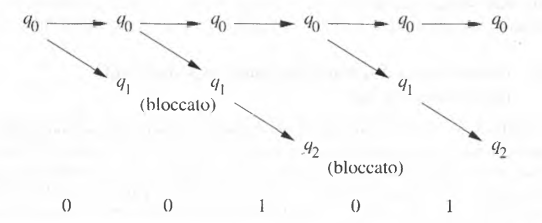
\includegraphics[scale=0.7]{img/nfa.png}
	\end{center}
	ovvero si parte dallo stato inziale, quando viene letto 0 si passa a $q_0$ e $q_1$, poi viene letto il secondo 0 quindi $q_0$ va nuovamente verso $q_0$ e $q_1$ mentre il primo $q_1$ muore non avendo transizioni su 0. Arriva poi l'1 quindi $q_0$ va solon verso $q_0$ e $q_1$ verso $q_2$ e sarebbe accettante ma l'input non è finito. Ora arriva 0 e $q_2$ si blocca mentre $q_0$ va sia in $q_0$ che in $q_1$. Arriva infine un 1 che manda $q_0$ in $q_0$ e $q_1$ in $q_2$ che è accettante e non avendo altri input si è dimostrata l'appartenenza della stringa al linguaggio
\end{example}
definisco quindi un NFA come una quintupla:
$A=(Q,\Sigma,\delta,q_0,F)$
con, a differenza dei DFA:
$\delta:Q\times F\to 2^Q$
Possiamo ora definire {$\delta$}, delta cappuccio che prende in ingresso uno stato e l'intera stringa $w$. Definisco ricorsivamente:
\begin{itemize}
	\item \textbf{caso base:} se $|w|=0$ ovvero se $W=\epsilon$ si ha:
	      $\hat{\delta}(q,\epsilon)=\{q\}$
	\item \textbf{caso passo:} se $|w|>0$, allora $W=xa$, $a\in\Sigma$ e $x\in\Sigma^*$. Posto $\hat{\delta}(q,x)=\{p_1,\cdots,p_k\}$ si ha:
	      $\hat{\delta}(q,w)=\cup \delta(p_i,a)$
\end{itemize}
%aggiungere esempio
Per il linguaggio $L$ accettato dall'automa si ha:
$L(A)=\{w\in \Sigma^*|\, \hat{\delta}(q_0,q)\cap F\neq \emptyset\}$
\begin{example}
	Automa per $L=\{x010y|\,x,y\in\{0,1\}^*\}$ ovvero tutte le stringhe con dentro la sequenza $010$:
	\begin{center}
		\begin{tikzpicture}[shorten >=1pt,node distance=2cm,on grid,auto]
			\node[state, initial] (q_0) {$q_{0}$};
			\node[state] (q_1) [right=of q_0] {$q_{1}$};
			\node[state] (q_2) [right=of q_1] {$q_{2}$};
			\node[state, accepting] (q_3) [right=of q_2] {$q_{3}$};
			\path[->]
			(q_0) edge  node {0} (q_1)
			edge [loop above] node {0,1} ()
			(q_1) edge  node {1} (q_2)
			(q_2) edge  node {0} (q_3)
			(q_3)     edge [loop above] node {0,1} ();
		\end{tikzpicture}
	\end{center}
\end{example}
Troviamo ora un algoritmo che trasformi un NFA in un DFA.\\
Dal penultimo esempio esempio ricavo:
\begin{center}
	\begin{tabular}{c|c|c}
		                     & 0             & 1             \\
		\hline
		$\emptyset$          & $\emptyset$   & $\emptyset$   \\
		\hline
		$\to \,\{q_0\}$      & $\{q_0,q_1\}$ & $\{q_0\}$     \\
		\hline
		$\,\{q_1\}$          & $\emptyset$   & $\{q_2\}$     \\
		\hline
		$*\,\{q_2\}$         & $\emptyset$   & $\emptyset$   \\
		\hline
		$\{q_0,q_1\}$        & $\{q_0,q_1\}$ & $\{q_0,q_2\}$ \\
		\hline
		$*\,\{q_0,q_2\}$     & $\{q_0,q_1\}$ & $\{q_0\}$     \\
		\hline
		$*\,\{q_1, q_2\}$    & $\emptyset$   & $\{q_2\}$     \\
		\hline
		$*\,\{q_0,q_1,q_2\}$ & $\{q_0,q_1\}$ & $\{q_0,q_2\}$
	\end{tabular}
\end{center}
ovvero:
\begin{center}
	\begin{tikzpicture}[shorten >=1pt,node distance=4cm,on grid,auto]
		\node[state, initial] (q_0) {$\{q_{0}\}$};
		\node[state] (q_1) [right=of q_0] {$\{q_{0}, q_1\}$};
		\node[state] (q_2) [right=of q_1] {$\{q_0,q_{2}\}$};
		\path[->]
		(q_0) edge  node {0} (q_1)
		edge [loop above] node {1} ()
		(q_1) edge  node {1} (q_2)
		edge [loop above] node {0} ()
		(q_2) edge [bend left =25]  node {0} (q_1)
		edge [bend left =45] node  {1} (q_0);
	\end{tikzpicture}
\end{center}
che è il DFA che si era anche prima ottenuto. Si hanno però dei sottoinsiemi mai raggiungibili. Si ha quindi:
\begin{center}
	\begin{tabular}{c|c|c}
		                 & 0             & 1             \\
		\hline
		$\to\,\{q_0\}$   & $\{q_0,q_1\}$ & $\{q_0\}$     \\
		\hline
		$\{q_0,q_1\}$    & $\{q_0,q_1\}$ & $\{q_0,q_2\}$ \\
		\hline
		$\,\{q_0, q_2\}$ & $\{q_0,q_1\}$ & $\{q_0\}$
	\end{tabular}
\end{center}
e definendo $\{q_0\}=a, \, \{q_0,q_1\}=b\,\,\, e\,\,\, \{q_0,q_2\}=c$ si avrà:
\begin{center}
	\begin{tikzpicture}[shorten >=1pt,node distance=2cm,on grid,auto]
		\node[state, initial] (q_0) {$a$};
		\node[state] (q_1) [right=of q_0] {$b$};
		\node[state, accepting] (q_2) [right=of q_1] {$c$};
		\path[->]
		(q_0) edge  node {0} (q_1)
		edge [loop above] node {1} ()
		(q_1) edge  node {1} (q_2)
		edge [loop above] node {0} ()
		(q_2) edge  [bend left =25] node {0} (q_1)
		edge [bend left = 50] node {1} (q_0);
	\end{tikzpicture}
\end{center}
Definiamo questo algoritmo che avrà:
\begin{itemize}
	\item come input un NFA $N=(Q_n,\Sigma,\delta_N,q_0,F_N)$
	\item come output un DFA $D=(Q_D,\Sigma,\delta_D,\{q_0\},F_D)$ tale che $L(D)=L(N)$
\end{itemize}
con:
\begin{itemize}
	\item $Q_D=2^{Q_N}$ (quindi se $Q_N=n$ si ha $|Q_D|=2^n$)
	\item $F_D=\{S\subseteq Q_n|\, S\cap F_N\neq \emptyset\}$
	\item $\forall S\subseteq Q_N$ e $ \forall a \in\Sigma$:
	      $\delta_D(S,a)=\cup \delta_n(p,a)$
	      per esempio:
	      $\delta_D(\{q_0,q_1,q_2\},0)=\delta_N(q_0,0)\cup \delta_N(q_1,0) \cup\delta_N(q_2,0) $
\end{itemize}
Si definisce l'$\epsilon-NFA$, l'automa astati finiti non deterministici con $\epsilon$ transizioni. Con la transizione $\epsilon$ posso saltare i nodi, ovvero avanza senza aggiungere caratteri
\begin{example}
	Si ha $ER=a^*b^*c^*$, che genera:
	$L=\{a^nb^mc^k|\,n,m,k\geq 0\}$
	si ha:
	\begin{center}
		\begin{tikzpicture}[shorten >=1pt,node distance=2cm,on grid,auto]
			\node[state, initial] (q_0) {$q_0$};
			\node[state] (q_1) [right=of q_0] {$q_1$};
			\node[state, accepting] (q_2) [right=of q_1] {$q_2$};
			\path[->]
			(q_0) edge  node {$\epsilon$} (q_1)
			edge [loop above] node {a} ()
			(q_1) edge  node {$\epsilon$} (q_2)
			edge [loop above] node {b} ()
			(q_2) edge  [loop above] node {c} ();
		\end{tikzpicture}
	\end{center}
	ovvero con $\epsilon$ posso per esempio generare quante $a$ voglio da $q_0$ e passare a $q_2$, uscendo senza generare altro
\end{example}
Si definisce la funzione $E\,CLOSE:Q\to 2^Q$, con $E\,CLOSE(q)$ insieme degli stati raggiungibili da $q$ tramite $\epsilon-mosse$. Nell'esempio precedente si avrebbe:
$E\,CLOSE(q_0)=\{q_0,q_1,q_2\}$
$E\,CLOSE(q_1)=\{q_1,q_2\}$
$E\,CLOSE(q_2)=\{q_2\}$
si ha inoltre che:
\begin{itemize}
	\item $E\,CLOSE 2^Q\to 2^Q\,\,\, P\subseteq Q$
	\item $E\,CLOSE(P)=\cup E\,CLOSE(p)$
	\item $E\,CLOSE(\emptyset)=\emptyset$
\end{itemize}
mettendo in tabella l'esempio precedente si ha:
\begin{center}
	\begin{tabular}{c|c|c|c}
		                        & a                 & b             & c           \\
		\hline
		$*\to\,\{q_0,q_1,q_2\}$ & $\{q_0,q_1,q_2\}$ & $\{q_1,q_2\}$ & $\{q_2\}$   \\
		\hline
		$*\{q_1,q_2\}$          & $\emptyset$       & $\{q_1,q_2\}$ & $\{q_2\}$   \\
		\hline
		$*\{q_2\}$              & $\emptyset$       & $\emptyset$   & $\{q_2\}$   \\
		\hline
		$\emptyset$             & $\emptyset$       & $\emptyset$   & $\emptyset$
	\end{tabular}
\end{center}
riscrivendo:
\begin{itemize}
	\item $a=\{q_0,q_1,q_2\}$
	\item $b=\{q_1,q_2\}$
	\item $c=\{q_2\}$
	\item $d=\emptyset$
\end{itemize}
ovvero:
$\delta_D(\{q_0,q_1,q_2\},a)=E\,CLOSE(\delta_N(q_0,a)\cup \delta_N(q_1,a)\cup \delta_N(q_2,a))$
$=E\,CLOSE(\{q_0\} \cup \emptyset\cup \emptyset)=E\,CLOSE(\{q_0\})$
$=E\,CLOSE	(q_0)=\{q_0,q_1,q_2\}$
e
$\delta_D(\{q_0,q_1,q_2\},B)=E\,CLOSE(\delta_N(q_0,b)\cup \delta_N(q_1,b)\cup \delta_N(q_2,b))$
$=E\,CLOSE(\emptyset \cup \{q_1\}\cup \emptyset)=E\,CLOSE(\{q_1\})$
$=E\,CLOSE	(q_1)=\{q_1,q_2\}$
e
$\delta_D(\{q_0,q_1,q_2\},c)=E\,CLOSE(\delta_N(q_0,c)\cup \delta_N(q_1,c)\cup \delta_N(q_2,c))$
$=E\,CLOSE(\emptyset \cup \emptyset\cup \{q_2\})=E\,CLOSE(\{q_1\})$
$=E\,CLOSE	(q_2)=\{q_2\}$

si ottiene quindi il seguente NFA:
\begin{center}
	\begin{tikzpicture}[shorten >=1pt,node distance=3cm,on grid,auto]
		\node[state, initial, accepting] (q_0) {$A$};
		\node[state, accepting] (q_1) [right=of q_0] {$B$};
		\node[state, accepting] (q_2) [below=of q_0] {$C$};
		\node[state] (q_3) [right=of q_2] {$D$};
		\path[->]
		(q_0) edge  node {b} (q_1)
		edge  node {c} (q_2)
		edge [loop above] node {a} ()
		(q_1) edge  node {c} (q_2)
		edge  node {a} (q_3)
		edge [loop above] node {b} ()
		(q_2) edge  node {a,b} (q_3)
		edge [loop below] node {c} ()
		(q_3) edge [loop below] node {a,b,c} ();
	\end{tikzpicture}
\end{center}
che diventa il seguente DFA:
\begin{center}
	\begin{tikzpicture}[shorten >=1pt,node distance=3cm,on grid,auto]
		\node[state, initial, accepting] (q_0) {$\{q_0,q_1,q_2\}$};
		\node[state, accepting] (q_1) [right=of q_0] {$\{q_1,q_2\}$};
		\node[state, accepting] (q_2) [below=of q_0] {$\{q_2\}$};
		\node[state] (q_3) [right=of q_2] {$q_E$};
		\path[->]
		(q_0) edge  node {b} (q_1)
		edge  node {c} (q_2)
		edge [loop above] node {a} ()
		(q_1) edge  node {c} (q_2)
		edge  node {a} (q_3)
		edge [loop above] node {b} ()
		(q_2) edge  node {a,b} (q_3)
		edge [loop below] node {c} ();
	\end{tikzpicture}
\end{center}

\subsubsection{esercizi}
\begin{example}
	automa DFA per $w=x010y,\,x,y\in\{0,1\}^*$ :\\
	la stringa più corta è 010
	\begin{center}
		\begin{tikzpicture}[shorten >=1pt,node distance=2cm,on grid,auto]
			\node[state, initial] (q_0) {$q_{0}$};
			\node[state] (q_1) [right=of q_0] {$q_{1}$};
			\node[state] (q_2) [right=of q_1] {$q_{2}$};
			\node[state, accepting] (q_3) [right=of q_2] {$q_{3}$};
			\path[->]
			(q_0) edge  node {0} (q_1)
			edge [loop above] node {1} ()
			(q_1) edge  node {1} (q_2)
			edge [loop above] node {0} ()
			(q_2) edge  node {0} (q_3)
			edge  [bend left = 45] node {1}(q_0)
			(q_3) edge [loop above] node {0,1} ();
		\end{tikzpicture}
	\end{center}
\end{example}
\begin{example}
	automa DFA per $a^{2k+1}b^{2h},\, h,k\geq 0$ :\\
	concatenazione di a dispari e b pari:
	\begin{center}
		\begin{tikzpicture}[shorten >=1pt,node distance=2cm,on grid,auto]
			\node[state, initial] (q_0) {$q_{0}$};
			\node[state, accepting] (q_1) [right=of q_0] {$q_{1}$};
			\node[state] (q_3) [right=of q_1] {$q_{3}$};
			\node[state] (q_2) [below= of q_1] {$q_{2}$};
			\node[state, accepting] (q_4) [right = of q_2] {$q_4$};
			\node[state] (q_5) [right=of q_4] {$q_E$};
			\path[->]
			(q_0) edge  node [bend left = 25] {a} (q_1)
			(q_1) edge [bend left = 25] node {a} (q_2)
			edge node [bend left= 25] {b} (q_3)
			(q_2) edge [bend left = 25] node [left] {a} (q_1)
			(q_3) edge [bend right = 25] node [left] {b} (q_4)
			(q_4) edge [bend right = 25] node [right] {b} (q_3)
			(q_2) edge  [bend right = 55] node [below] {b} (q_5)
			(q_3) edge  [bend left = 25] node {a} (q_5)
			(q_4) edge  [bend right = 25] node [below] {a} (q_5)
			(q_5) edge [loop right] node {a,b} ();
		\end{tikzpicture}
	\end{center}
\end{example}
\begin{example}
	cerco DFA per stringhe inizianti con a e finenti con b, con occorrenze di b singole o a coppie, nessuna regola per c.\\
	per esempio $abbcb$ è nel linguaggio
	\begin{center}
		\begin{tikzpicture}[shorten >=1pt,node distance=2cm,on grid,auto]
			\node[state, initial] (q_0) {$q_{0}$};
			\node[state] (q_1) [right=of q_0] {$q_{1}$};
			\node[state, accepting] (q_2) [right=of q_1] {$q_{2}$};
			\node[state, accepting] (q_3) [right= of q_3] {$q_{3}$};
			\node[state] (q_5) [below=of q_0] {$q_E$};
			\path[->]
			(q_0) edge  node [bend left = 25] {a} (q_1)
			edge  node [bend left = 25] {b,c} (q_5)
			(q_1) edge  node {b} (q_2)
			edge [loop] node {a,c} ()
			(q_2) edge [bend left = 25] node {a,c} (q_1)
			edge  node  {b} (q_3)
			(q_3) edge [bend left = 65] node [below] {b} (q_5)
			edge [bend left = 55] node {a,c} (q_1)
			(q_5) edge [loop left] node {a,b,c} ();
		\end{tikzpicture}
	\end{center}
\end{example}

\begin{example}
	cerco DFA per  stringhe di bit non contegano 000
	\begin{center}
		\begin{tikzpicture}[shorten >=1pt,node distance=2cm,on grid,auto]
			\node[state, initial, accepting] (q_0) {$q_0$};
			\node[state, accepting] (q_1) [right=of q_0]{$q_1$};
			\node[state, accepting] (q_2) [right=of q_1]{$q_2$};
			\node[state] (q_e) [right=of q_2]{$q_E$};
			\path[->]
			(q_0) edge  [bend left=25] node {0} (q_1)
			edge [loop] node {1} ()
			(q_1) edge node {0} (q_2)
			edge [bend left=25] node {1} (q_0)
			(q_2) edge node {0} (q_e)
			edge  [bend left=55] node{1} (q_0)
			(q_e) edge [loop ] node {0,1} ();
		\end{tikzpicture}
	\end{center}
\end{example}
\begin{example}
	cerco DFA per  stringhe di bit non contegano 000 almeno una volta
	\begin{center}
		\begin{tikzpicture}[shorten >=1pt,node distance=2cm,on grid,auto]
			\node[state, initial] (q_0) {$q_0$};
			\node[state] (q_1) [right=of q_0]{$q_1$};
			\node[state] (q_2) [right=of q_1]{$q_2$};
			\node[state, accepting] (q_e) [right=of q_2]{$q_E$};
			\path[->]
			(q_0) edge  [bend left=25] node {0} (q_1)
			edge [loop] node {1} ()
			(q_1) edge node {0} (q_2)
			edge [bend left=25] node {1} (q_0)
			(q_2) edge node {0} (q_e)
			edge  [bend left=55] node{1} (q_0)
			(q_e) edge [loop ] node {0,1} ();
		\end{tikzpicture}
	\end{center}
\end{example}
\begin{example}
	cerco DFA per  stringhe di bit che contengono 000 solo una volta
	\begin{center}
		\begin{tikzpicture}[shorten >=1pt,node distance=2cm,on grid,auto]
			\node[state, initial] (q_0) {$q_0$};
			\node[state] (q_1) [right=of q_0]{$q_1$};
			\node[state] (q_2) [right=of q_1]{$q_2$};
			\node[state, accepting] (q_3) [right=of q_2]{$q_3$};
			\node[state,accepting] (q_4) [below=of q_3] {$q_3$};
			\node[state] (q_5) [below=of q_4]{$q_5$};
			\node[state] (q_6) [below=of q_5]{$q_6$};
			\node[state] (q_e) [right=of q_3]{$q_E$};
			\path[->]
			(q_0) edge  [bend left=25] node {0} (q_1)
			edge [loop] node {1} ()
			(q_1) edge node {0} (q_2)
			edge [bend left=25] node {1} (q_0)
			(q_2) edge node {0} (q_3)
			edge  [bend left=45] node{1} (q_0)
			(q_3) edge node {0} (q_e)
			edge node {1} (q_4)
			(q_4) edge [bend left=25] node {0} (q_5)
			edge [loop right] node {1} ()
			(q_5) edge [bend left=25] node {1} (q_4)
			edge node {0} (q_6)
			(q_6) edge [bend right=25] node {0} (q_e)
			edge [bend left=55] node {0} (q_4)
			(q_e) edge [loop ] node {0,1} ();
		\end{tikzpicture}
	\end{center}
\end{example}

\begin{example}
	Trasformare il seguente NFA in un DFA:
	\begin{center}
		\begin{tikzpicture}[shorten >=1pt,node distance=3cm,on grid,auto]
			\node[state, initial, accepting] (q_0) {$q_0$};
			\node[state, accepting] (q_1) [above right=of q_0] {$q_1$};
			\node[state] (q_2) [below right =of q_0] {$q_2$};
			\node[state] (q_3) [below right=of q_1] {$q_3$};
			\path[->]
			(q_0) edge  [bend left=25] node {a} (q_1)
			edge  [bend right=25] node [below] {b} (q_2)
			(q_1) edge  [bend left=25] node {a} (q_2)
			edge [loop ] node {a} ()
			(q_2) edge  [bend left=25] node {b} (q_1)
			edge  [bend right=15] node [below] {b} (q_3)
			(q_3) edge   node [above] {a} (q_1)
			edge  [bend right=15] node [above] {a} (q_2);
		\end{tikzpicture}
	\end{center}
	abbiamo quindi:
	$\delta_D(\{q_0\},a)=\delta_N(q_0,a)=\{q_1,q_2\}$
	$\delta_D(\{q_0\},b)=\delta_N(q_1,b)=\emptyset$
	$\delta_D(\{q_1,q_2\},a)=\delta_N(q_1,a)\cup \delta_N(q_2,a)=\{q_1,q_2\}cup \emptyset=\{q_1,q_2\}$
	$\delta_D(\{q_1,q_2\},b)=\delta_N(q_1,b)\cup \delta_N(q_2,b)=\emptyset\cup \{q_1,q_3\}=\{q_1,q_3\}$
	$\cdots$
	ottengo quindi:
	\begin{center}
		\begin{tabular}{c|c|c}
			DFA             & a             & b             \\
			\hline
			$*\to\,\{q_0\}$ & $\{q_1,q_2\}$ & $\emptyset$   \\
			\hline
			$*\{q_1,q_2\}$  & $\{q_1,q_2\}$ & $\{q_1,q_3\}$ \\
			\hline
			$\emptyset$     & $\emptyset$   & $\emptyset$   \\
			\hline
			$*\{q_1,q_3\}$  & $\{q_1,q_2\}$ & $\emptyset$
		\end{tabular}
	\end{center}
	Posso ora rinominare:
	\begin{itemize}
		\item $A=\{q_0\}$
		\item $B=\{q_1,q_2\}$
		\item $C=\emptyset$
		\item $D=\{q_1,q_3\}$
	\end{itemize}

	ottengo quindi il seguente DFA:
	\begin{center}
		\begin{tikzpicture}[shorten >=1pt,node distance=3cm,on grid,auto]
			\node[state, initial, accepting] (q_0) {$A$};
			\node[state, accepting] (q_1) [right=of q_0] {$B$};
			\node[state] (q_2) [below=of q_0] {$C$};
			\node[state,accepting] (q_3) [right=of q_2] {$D$};
			\path[->]
			(q_0) edge  node {a} (q_1)
			edge  node {b} (q_2)
			(q_1) edge  [bend left=25] node {b} (q_3)
			edge  [loop] node {a} ()
			(q_2) edge  [loop below] node {a,b} ()
			(q_3) edge  [bend left=25] node {a} (q_1)
			edge  node  {a} (q_2);
		\end{tikzpicture}
	\end{center}
\end{example}
\begin{example}
	Trasformare il seguente $\epsilon$-NFA in un DFA:
	\begin{center}
		\begin{tikzpicture}[shorten >=1pt,node distance=3cm,on grid,auto]
			\node[state, initial] (q_0) {$p$};
			\node[state] (q_1) [right=of q_0] {$q$};
			\node[state, accepting] (q_2) [below right =of q_0] {$r$};
			\path[->]
			(q_0) edge  [bend left=25] node [left] {c} (q_2)
			edge  [bend right=25] node {b} (q_1)
			edge [loop ] node {a} ()
			(q_1) edge  [bend right=25] node {$\epsilon$} (q_0)
			edge  [bend right=25] node [left] {b} (q_2)
			edge  [loop ] node {a} ()
			(q_2) edge  [bend left=25] node {c} (q_0)
			edge  [bend right=25] node [right] {$\epsilon$} (q_1)
			edge  [loop below] node {a} ();
		\end{tikzpicture}
	\end{center}
	vediamo le ECLOSE:
	$ECLOSE(p)=\{p\}$
	$ECLOSE(q)=\{p,q\}$
	$ECLOSE(r)=\{p,q,r\}$
	si ottiene quindi:
	\begin{center}
		\begin{tabular}{c|c|c|c}
			             & a           & b           & c           \\
			\hline
			$to\,\{p\}$  & $\{p\}$     & $\{p,q\}$   & $\{p,q,r\}$ \\
			\hline
			$\{p,q\}$    & $\{p,q\}$   & $\{p,q,r\}$ & $\{p,q,r\}$ \\
			\hline
			$*\{p,q,r\}$ & $\{p,q,r\}$ & $\{p,q,r\}$ & $\{p,q,r\}$
		\end{tabular}
	\end{center}
	infatti, per esempio:
	$\delta_D(\{p\}, a)= ECLOSE (\delta_(p,a))=ECLOSE (\{p\})=ECLOSE (p)=\{p\}$
	$\delta_D(\{p,q\}, a)= ECLOSE (\delta_N(p,a)\cup \delta_N(q,a))=$
	$ECLOSE (\{p\}\cup \{q\})=ECLOSE(P)\cup ECLOSE(q)=\{p\}\cup\{p,q\}=\{p,q\}$
	$\cdots$
	si hanno quindi le seguenti rinominazioni:
	\begin{itemize}
		\item $A=\{p\}$
		\item $b=\{p,q\}$
		\item $C=\{p,q,r\}$
	\end{itemize}
	ovvero:
	\begin{center}
		\begin{tikzpicture}[shorten >=1pt,node distance=3cm,on grid,auto]
			\node[state, initial] (q_0) {$A$};
			\node[state] (q_1) [right=of q_0] {$B$};
			\node[state, accepting] (q_2) [below=of q_0] {$C$};
			\path[->]
			(q_0) edge  node {b} (q_1)
			edge  node {c} (q_2)
			edge  [loop] node {a} ()
			(q_1) edge  node {b,c} (q_2)
			edge  [loop] node {a} ()
			(q_2) edge  [loop below] node {a,b,c} ();
		\end{tikzpicture}
	\end{center}
\end{example}

torniamo a dare bene qualche definizione per {$\delta$} in un DFA:
\begin{center}
	$\delta:Q\times \Sigma^* \to Q$
\end{center}
con: $q\in Q,\,\,\, w\in \Sigma^*\,\,\,e\,\,\,${$\delta$}$(p,w)=q$
\begin{itemize}
	\item
	      \textbf{caso base:} $w=\epsilon\to |w|=0\to${$\delta$}$(q,\epsilon)=q$
	      \\
	      \textbf{caso passo:} $|w|\neq0\to w=ax$ con $a\in \Sigma,x\in \Sigma^*$:
	      {$\delta$}$(q,w)=${$\delta$}$(q,ax)=${$\delta$} $(\delta(q,a),x)$
	\item
	      \textbf{caso base:} $w=\epsilon\to |w|=0\to \delta(q,w)=\delta(q,\epsilon)=q$
	      \\
	      \textbf{caso passo:} $|w|\neq0\to w=xa$ con $a\in \Sigma,x\in \Sigma^*$:
	      {$\delta$}$(q,w)=${$\delta$}$(q,xa)=${$\delta$} $(\delta(q,x),a)$
\end{itemize}
in un NFA si ha:
\begin{itemize}
	\item \textbf{caso base:}  {$\delta$}$(q,\epsilon=\{q\},\,\,\forall q\in Q$
	\item \textbf{caso passo:} posto $w=ax$ e {$\delta$}$(q,a)=\{p_1,\cdots,p_n$ allora {$\delta$}$(q,w)=\cup${$\delta$}$(p_i, x)0\{r_1,\cdots,r_n\}$.\\
	      {$\delta$}$(q,a)=p$\\
	      {$\delta$}$(q,w)=$ {$\delta$}$(q,xa)=$ {$\delta$}$(p,x)=r$
\end{itemize}
oppure:
\begin{itemize}
	\item \textbf{caso base:}  {$\delta$}$(q,\epsilon)=\{q\},\,\forall q\in Q$
	\item \textbf{caso passo:} posto $w=xa$ si ha  {$\delta$}$(q,q)=$ {$\delta$}$(q,xa)=\cup \delta(p,a)$ con  {$\delta$}$(q,x)=\{p_1,\cdots,p_n\}$
\end{itemize}
Se ho un NFA $N=(Q_N, \Sigma, \delta_N, q_{0_N}, F_N)$ con $\delta_N: Q\times\Sigma^*\to 2^{Q_N}$ che accetta un lingiaggio $L$ posso ottenere un DFA $D=(Q_D, \Sigma, \delta_D, q_{0_D}, F_D)$ equivalente con $Q_D=2^{Q_N}$  e $q_{0_D}=\{q_{0_N}\}$ che accetta L.\\
$\forall S\subseteq Q_N$ e $\forall a\in \Sigma$ si ha:
$F_D=\{S\subseteq Q_N\,|\, S\cap F_n\neq \emptyset\}$
con $\delta_D(S,a)=\cup \delta_N(p,a)$
Si ha che:
$|Q_D|=|2^{Q_N}|=2^{|Q_N|}$
partiamo con un esempio:
\begin{center}
	\begin{tikzpicture}[shorten >=1pt,node distance=2cm,on grid,auto]
		gin{tikzpicture}[shorten >=1pt,node distance=2cm,on grid,auto]
		\node[state,initial] (q_0)   {$q_0$};
		\node[state] (q_1) [right=of q_0] {$q_1$};
		\node[state] (q_2) [right=of q_1] {$\cdots$};
		\node[state] (q_3) [right=of q_2] {$q_{n-1}$};
		\node[state, accepting] (q_4) [right=of q_3] {$q_n$};
		\path[->]
		(q_0) edge  node {1} (q_1)
		edge [loop above] node {0,1} ()
		(q_1) edge  node {0,1} (q_2)
		(q_2) edge node {0,1} (q_3)
		(q_3) edge node {0,1} (q_4);
	\end{tikzpicture}
\end{center}
che definisce un $L\subseteq\{0,1\}^*$ tale che $w\in L$ sse n-simo elemento della fine è 1. Si ha:
$|Q_N|=n+1\to |Q_D|=2^n$
Si ha che dato un $\epsilon$-NFA $E=(Q_E, \Sigma, \delta_E, q_{0_E}, F_E)$ che riconosce $L$ in un NFA $N=(Q_N, \Sigma, \delta_N, q_{0_N}, F_N)$ equivalenti con $Q_N=2^{Q_E}$ stati in $Q_E$ $\epsilon$-close: \textit{ECLOSE(S)=S} e $q_N=ECLOSE(q_E)$:
$F_N\{S\in Q_F,\,\, S\subseteq Q_E | S\cap F_E\neq \emptyset\}$
quindi:
$\forall a\in \Sigma \text{ e } \forall S=\{p_1,\cdots,p_k\}, \forall S\in Q_F \text{ e } Q_E$
$\delta_F(S,a) \text{ si ottiene }\cup \delta_E(p_i,a)=\{r_1,\cdots, r_n\}$
$\delta_N(S,a)=ECLOSE(\{r_1, \cdots, r_n\})$

\begin{Exercise}\label{exe:no-101-er}
Costruire un'espressione regolare per il linguaggio $L\in\Sigma_{B}$ delle parole che non contengono la sottostringa \texttt{101}.
\end{Exercise}

\begin{Answer}
Una possibilità, che verrà formalizzata in \Cref{sec:da-DFA-a-ER} consiste nel partire dal DFA che riconosce il
linguaggio e sintetizzare l'espressione regolare a partire dall'automa.

Per ottenere un'ER semplice è invece preferibile ragionare sulla definizione di linguaggio da esprimere.
Una definizione equivalente è l'insieme delle parole in cui ogni occorrenza del carattere \texttt{1} è seguita da un
altro \texttt{1}, oppure da \texttt{00}, oppure ancora tale \texttt{1} è uno degli ultimi due caratteri della parola (in
questo caso, non potrà essere il carattere iniziale di una sottostringa \texttt{101})
Questa formulazione si presta maggiormente a disegnare un'espressione regolare.
Infatti, una riscrittura diretta di quanto descritto sopra, tenendo presente che un numero arbitrari di \texttt{0}
potrebbe precedere il primo \texttt{1} e seguire ogni \texttt{0}, diventa
$$\texttt{0}^{*}(\texttt{100}\texttt{0}^{*})^{*} (\texttt{10} |\texttt{1} | \epsilon)$$ che può essere ulteriormente
semplificata in
$$\texttt{0}^{*}(\texttt{100}\texttt{0}^{*})^{*} \texttt{1}^{*} \texttt{0}^{*}.$$
\end{Answer}



\begin{Exercise}\label{exe:no-diff2-er}
Costruire un'espressione regolare per il linguaggio $L\in\Sigma_{B}$ delle parole che soddisfano le due seguenti
condizioni:
\begin{enumerate}
\item hanno lo stesso numero di \zero e \uno
\item in ogni prefisso il numero di \zero e \uno differisce al massimo di $1$.
\end{enumerate}
Sono quindi parole del linguaggio $\epsilon$, \zero\uno, \texttt{10}, \texttt{101010}, \texttt{0101}.
Non sono parole del linguaggio \texttt{1100}.
\end{Exercise}

\begin{Exercise}\label{exe:3x3}
Costruire un'espressione regolare per il linguaggio $L\in\Sigma_{B}$ delle parole con un numero di \zero multiplo di $3$ e
un numero di \uno multiplo di $3$.
\end{Exercise}


\section{Da DFA a espressioni regolari}
\label{sec:da-DFA-a-ER}

\begin{itemize}
	\item \textbf{caso base}:
	      \begin{enumerate}
		      \item se $R=\epsilon$ ovvero $L(R)=\{\epsilon\}$ allora:
		            \begin{center}
			            \begin{tikzpicture}[shorten >=1pt,node distance=2cm,on grid,auto]
				            \node[state,initial] (q_0)   {$q_0$};
				            \node[state, accepting] (q_1) [right=of q_0] {$q_1$};
				            \path[->]
				            (q_0) edge node {$\epsilon$} (q_1);
			            \end{tikzpicture}
		            \end{center}
		      \item se $R=\emptyset$ ovvero $L(R)=\emptyset$ allora:
		            \begin{center}
			            \begin{tikzpicture}[shorten >=1pt,node distance=2cm,on grid,auto]
				            \node[state,initial] (q_0)   {$q_0$};
				            \node[state, accepting] (q_1) [right=of q_0] {$q_1$}; ;
			            \end{tikzpicture}
		            \end{center}
		      \item se $R=a$ ovvero $L(R)=\{a\}$ allora:
		            \begin{center}
			            \begin{tikzpicture}[shorten >=1pt,node distance=2cm,on grid,auto]
				            \node[state,initial] (q_0)   {$q_0$};
				            \node[state, accepting] (q_1) [right=of q_0] {$q_1$};
				            \path[->]
				            (q_0) edge node {a} (q_1);
			            \end{tikzpicture}
		            \end{center}
	      \end{enumerate}
	\item \textbf{caso passo:}
	      \begin{enumerate}
		      \item se $R=S+T$ quindi $L(R)=L(S)+L(T)$ allora:
		            \begin{center}
			            \begin{tikzpicture}[shorten >=1pt,node distance=2cm,on grid,auto]
				            \node[state,initial] (q_0)   {$q_0$};
				            \node[state] (q_1) [above right =of q_0] {$q_1$};
				            \node[state] (q_2) [below right =of q_0] {$q_2$};
				            \node[draw=none,fill=none] (Q_E) [right = of q_1] {$S$};
				            \node[draw=none,fill=none] (Q_F) [right = of q_2] {$S$};
				            \node[state] (q_3) [right=of Q_E] {$q_3$};
				            \node[state] (q_4) [right=of Q_F] {$q_4$};
				            \node[state, accepting] (q_5) [below right =of q_3] {$q_5$};
				            \path[->]
				            (q_0) edge node {$\epsilon$} (q_1)
				            (q_0) edge node {$\epsilon$} (q_2)
				            (q_3) edge node {$\epsilon$} (q_5)
				            (q_4) edge node {$\epsilon$} (q_5);
			            \end{tikzpicture}
		            \end{center}
		      \item se $R=ST$ quindi $L(R)=L(S)L(T)$:
		            \begin{center}
			            \begin{tikzpicture}[shorten >=1pt,node distance=2cm,on grid,auto]
				            \node[state,initial] (q_0)   {$q_0$};
				            \node[draw=none,fill=none] (Q_E) [right = of q_0] {$S$};
				            \node[state] (q_1) [ right =of Q_E] {$q_1$};
				            \node[state] (q_2) [right =of q_1] {$q_2$};
				            \node[draw=none,fill=none] (Q_F) [right = of q_2] {$T$};
				            \node[state] (q_3) [right=of Q_F] {$q_3$};
				            \node[draw=none,fill=none] (Q_G) [right = of q_3] {};
				            \path[->]
				            (q_1) edge node {$\epsilon$} (q_2)
				            (q_3) edge node {} (Q_G);
			            \end{tikzpicture}
		            \end{center}
		      \item se $R=S^*$ quindi $L(R)=(L(S))^*$:
		            \begin{center}
			            \begin{tikzpicture}[shorten >=1pt,node distance=2cm,on grid,auto]
				            \node[state,initial] (q_0)   {$q_0$};
				            \node[state] (q_1) [ right =of Q_E] {$q_1$};
				            \node[draw=none,fill=none] (Q_F) [right = of q_1] {$S$};
				            \node[state] (q_2) [right =of Q_F] {$q_2$};
				            \node[state] (q_3) [right=of q_2] {$q_3$};
				            \path[->]
				            (q_0) edge node {$\epsilon$} (q_1)
				            (q_2) edge [bend right = 35]  node {$\epsilon$} (q_1)
				            (q_0) edge [bend right = 25] node  {$\epsilon$} (q_3)
				            (q_2) edge node {$\epsilon$} (q_3);
			            \end{tikzpicture}
		            \end{center}
	      \end{enumerate}
\end{itemize}




\begin{example}
	creo E-NFA per
	$ER=(0+1)^*1(0+1)$
	si ha che per 0+1:
	\begin{center}
		\begin{tikzpicture}[shorten >=1pt,node distance=2cm,on grid,auto]
			\node[state,initial] (q_0)   {$q_0$};
			\node[state] (q_1) [above right =of q_0] {$q_1$};
			\node[state] (q_2) [below right =of q_0] {$q_2$};
			\node[state] (q_3) [right=of q_1] {$q_3$};
			\node[state] (q_4) [right=of q_2] {$q_4$};
			\node[state] (q_5) [below right =of q_3] {$q_5$};
			\path[->]
			(q_0) edge node {$\epsilon$} (q_1)
			(q_0) edge node {$\epsilon$} (q_2)
			(q_1) edge node {$0$} (q_3)
			(q_2) edge node {$1$} (q_4)
			(q_3) edge node {$\epsilon$} (q_5)
			(q_4) edge node {$\epsilon$} (q_5);
		\end{tikzpicture}
	\end{center}
	da qui ottengo $(0+1)^*$
	\begin{center}
		\begin{tikzpicture}[shorten >=1pt,node distance=2cm,on grid,auto]
			\node[state, initial] (q_i)   {$q_i$};
			\node[state] (q_0) [right of = q_i]  {$q_0$};
			\node[state] (q_1) [above right =of q_0] {$q_1$};
			\node[state] (q_2) [below right =of q_0] {$q_2$};
			\node[state] (q_3) [right=of q_1] {$q_3$};
			\node[state] (q_4) [right=of q_2] {$q_4$};
			\node[state] (q_5) [below right =of q_3] {$q_5$};
			\node[state, accepting] [right of =q_5] (q_f)   {$q_f$};
			\path[->]
			(q_i) edge node {$\epsilon$} (q_0)
			(q_i) edge [bend right =65] node {$\epsilon$} (q_f)
			(q_0) edge node {$\epsilon$} (q_1)
			(q_0) edge node {$\epsilon$} (q_2)
			(q_1) edge node {$0$} (q_3)
			(q_5) edge  [bend right =100] node [above] {$\epsilon$} (q_0)
			(q_2) edge node {$1$} (q_4)
			(q_3) edge node {$\epsilon$} (q_5)
			(q_5) edge node {$\epsilon$} (q_f)
			(q_4) edge node {$\epsilon$} (q_5);
		\end{tikzpicture}
	\end{center}
	unisco e aggiungo uno nel mezzo:
	\begin{center}
		\begin{tikzpicture}[shorten >=1pt,node distance=1.4cm,on grid,auto]
			\node[state, initial] (q_i)   {$q_i$};
			\node[state] (q_0) [right of = q_i]  {$q_0$};
			\node[state] (q_1) [above right =of q_0] {$q_1$};
			\node[state] (q_2) [below right =of q_0] {$q_2$};
			\node[state] (q_3) [right=of q_1] {$q_3$};
			\node[state] (q_4) [right=of q_2] {$q_4$};
			\node[state] (q_5) [below right =of q_3] {$q_5$};
			\node[state] (q_f) [below right =of q_5] {$q_f$};

			\node[state] (q_m) [right of = q_f]  {$q_m$};
			\node[state] (q_n) [right =of q_m] {$q_n$};

			\node[state] (q_6) [right of = q_n]  {$q_6$};
			\node[state] (q_7) [above right =of q_6] {$q_7$};
			\node[state] (q_8) [below right =of q_6] {$q_8$};
			\node[state] (q_9) [right=of q_7] {$q_9$};
			\node[state] (q_a) [right=of q_8] {$q_a$};
			\node[state] (q_b) [below right =of q_9] {$q_b$};
			\path[->]
			(q_i) edge node {$\epsilon$} (q_0)
			(q_i) edge [bend right =65] node {$\epsilon$} (q_f)
			(q_0) edge node {$\epsilon$} (q_1)
			(q_0) edge node {$\epsilon$} (q_2)
			(q_1) edge node {$0$} (q_3)
			(q_5) edge  [bend right =100] node [above] {$\epsilon$} (q_0)
			(q_2) edge node {$1$} (q_4)
			(q_3) edge node {$\epsilon$} (q_5)
			(q_5) edge node {$\epsilon$} (q_f)
			(q_4) edge node {$\epsilon$} (q_5)
			(q_f) edge node  {$\epsilon$} (q_m)
			(q_m) edge node  {$1$} (q_n)
			(q_n) edge node  {$\epsilon$} (q_6)
			(q_6) edge node {$\epsilon$} (q_7)
			(q_6) edge node {$\epsilon$} (q_8)
			(q_6) edge node {$0$} (q_8)
			(q_7) edge node {$1$} (q_9)
			(q_8) edge node {$\epsilon$} (q_a)
			(q_a) edge node {$\epsilon$} (q_b)
			(q_9) edge node {$\epsilon$} (q_b);
		\end{tikzpicture}
	\end{center}
\end{example}
Vediamo ora l'algoritmo che trasforma DFA in una ER. Questo algoritmo permette di verificare quale linguaggio è accettato o meno dall'automa:\\
dato DFA $A=(Q,\Sigma, \delta, q_0,F)$ con $Q$ e $F$ stati non finali e $Q$, $F$, $q_0$ che sono i primi stati da eliminare. L'algoritmo procede per eliminazioni successive. Si costruisce quindi l'automa $B$ che ha solo $q_0$ e $F=\{q_1,\cdots,q_k\}$. Scrivo quindi $K$ espressioni regolari considerando solo $q_0$ e il k-esimo stato finale eliminando pian piano gli altri stati. Alla fine ottengo le varie espressioni regolari da unire:
$E=E1+E2+\cdots+Ek$
vediamo ora come eliminare uno stato. Partiamo dal seguente automa:
\begin{center}
	\begin{tikzpicture}[shorten >=1pt,node distance=4cm,on grid,auto]
		\node[state] (q_1)   {$q_1$};
		\node[state] (s) [below right =of q_1] {$s$};
		\node[state] (q_k) [below left =of s] {$q_k$};
		\node[state] (p_1) [above right=of s] {$p_1$};
		\node[state] (p_m) [below right =of s] {$p_m$};
		\path[->]
		(q_1) edge node {$Q_1$} (s)
		(q_1) edge [bend left =50] node {$R_{11}$} (p_1)
		(q_1) edge [bend left =100] node {$R_{1m}$} (p_m)
		(s)   edge node {$p_1$} (p_1)
		(s)   edge node {$p_m$} (p_m)
		(s)   edge [loop above] node {$S$} ()
		(q_k) edge node {$Q_k$} (s)
		(q_k) edge [bend right =50] node {$R_{k1}$} (p_1)
		(q_k) edge [bend right =100] node {$R_{km}$} (p_m);
	\end{tikzpicture}
\end{center}

ed elimino $s$:
\begin{center}
	\begin{tikzpicture}[shorten >=1pt,node distance=4cm,on grid,auto]
		\node[state] (q_1)   {$q_1$};
		\node[state] (q_k) [below =of q_1] {$q_k$};
		\node[state] (p_1) [right=of q_1] {$p_1$};
		\node[state] (p_m) [below  =of p_1] {$p_m$};
		\path[->]
		(q_1) edge node {$R_{11}+Q_1S^{*}P_1$} (p_1)
		(q_1) edge node [right]{$R_{1m}+Q_1S^{*}P_m$} (p_m)
		(q_k) edge node [left]{$R_{k1}+Q_kS^{*}P_1$} (p_1)
		(q_k) edge node {$R_{km}+Q_kS^{*}P_m$} (p_m);
	\end{tikzpicture}
\end{center}
quindi quando si ha uno stato iniziale $q_0$ e uno finale $q_1$:
\begin{itemize}
	\item se $q_0\neq q_1$:
	      \begin{center}
		      \begin{tikzpicture}[shorten >=1pt,node distance=3cm,on grid,auto]
			      \node[state, initial] (q_0)   {$q_1$};
			      \node[state, accepting] (q_1) [right=of q_1] {$q_k$};
			      \path[->]
			      (q_0) edge [bend left =25]node {$S$} (q_1)
			      (q_1) edge [bend left =25]node {$T$} (q_0)
			      (q_0)   edge [loop above] node {$R$} ()
			      (q_1)   edge [loop above] node {$U$} ();
		      \end{tikzpicture}
	      \end{center}
	      rappresenta:
	      $E_i=(R+SU^{*}T)^{*}SU^{*}$
	\item se $q_0=q$:
	      \begin{center}
		      \begin{tikzpicture}[shorten >=1pt,node distance=3cm,on grid,auto]
			      \node[state, initial, accepting] (q_0)   {$q_1$};
			      \path[->]
			      (q_0)   edge [loop above] node {$R$} ();
		      \end{tikzpicture}
	      \end{center}
	      rappresenta:
	      $E_i=R^{*}$
\end{itemize}

\begin{example}
	passo dall'automa a l'espressione regolare:
	\begin{center}
		\begin{tikzpicture}[shorten >=1pt,node distance=2cm,on grid,auto]
			\node[state, initial] (q_0) {$A$};
			\node[state] (q_1) [right=of q_0] {$B$};
			\node[state, accepting] (q_2) [right=of q_1] {$C$};
			\node[state, accepting] (q_3) [right=of q_2] {$D$};
			\path[->]
			(q_0) edge  node {1} (q_1)
			edge [loop above] node {0,1} ()
			(q_1) edge  node {0,1} (q_2)
			(q_2) edge  node {0,1} (q_3);
		\end{tikzpicture}
	\end{center}
	questo automa accetta le stringhe binarie con un uno in penultima o terzultima posizione.\\
	Rietichetto con le ER:
	\begin{center}
		\begin{tikzpicture}[shorten >=1pt,node distance=2cm,on grid,auto]
			\node[state, initial] (q_0) {$A$};
			\node[state] (q_1) [right=of q_0] {$B$};
			\node[state, accepting] (q_2) [right=of q_1] {$C$};
			\node[state, accepting] (q_3) [right=of q_2] {$D$};
			\path[->]
			(q_0) edge  node {1} (q_1)
			edge [loop above] node {0+1} ()
			(q_1) edge  node {0+1} (q_2)
			(q_2) edge  node {0+1} (q_3);
		\end{tikzpicture}
	\end{center}
	elimino B che non è iniziale o finale . Il predecessore di B è A e il successore è C. Si ha quindi:
	$A\to B:1$
	$B\to C:0+1$
	e non ho loop in B ($\emptyset$) e nessun arco tra A e C ($R_{a,c}=\emptyset$). Quindi:
	$R_{A,C}^{'}=\emptyset+1\emptyset^*(0+1)=1(0+1)$
	ovvero:
	\begin{center}
		\begin{tikzpicture}[shorten >=1pt,node distance=3cm,on grid,auto]
			\node[state, initial] (q_0) {$A$};
			\node[state, accepting] (q_2) [right=of q_0] {$C$};
			\node[state, accepting] (q_3) [right=of q_2] {$D$};
			\path[->]
			(q_0) edge  node {1(0+1)} (q_2)
			edge [loop above] node {0+1} ()
			(q_2) edge  node {0+1} (q_3);
		\end{tikzpicture}
	\end{center}
	Ho ora solo stati iniziali e finali, quindi $E=E_1+E_2$.
	Trovo $E1$, elimino quindi C. Si ha:
	$A\to C:1(0+1)$
	$C\to D:0+1$
	e non ho loop in B ($\emptyset$) e nessun arco tra A e D($R_{A,D}=\emptyset$), ovvero:
	$R_{A,D}=\emptyset+1(0+1)\emptyset^*(0+1)=1(0+1)(0+1)$
	che è:
	\begin{center}
		\begin{tikzpicture}[shorten >=1pt,node distance=4cm,on grid,auto]
			\node[state, initial] (q_0) {$A$};
			\node[state, accepting] (q_3) [right=of q_0] {$D$};
			\path[->]
			(q_0) edge  node {1(0+1)(0+1)} (q_3)
			edge [loop above] node {0+1} ();
		\end{tikzpicture}
	\end{center}
	quindi:
	$E_1=((0+1)+1(0+1)(0+1)\emptyset^*\emptyset)^*1(0+1)(0+1)\emptyset^*=(0+1)^*1(0+1)(0+1)$
	ottengo $E2$ eliminando D che non ha successori, quindi:
	$E_2=(0+1)^*1(0+1)$
	e quindi infine:
	$E=E_1+E_2=(0+1)^*1(0+1)(0+1)+(0+1)^*1(0+1)=(0+1)^*1(0+1)(\epsilon+0+1)$
\end{example}
\begin{example}
	\begin{center}
		\begin{tikzpicture}[shorten >=1pt,node distance=3cm,on grid,auto]
			\node[state, initial, accepting] (q_0) {$p$};
			\node[state] (q_1) [right =of q_0] {$s$};
			\node[state] (q_2) [right=of q_1] {$r$};
			\node[state] (q_3) [below=of q_1] {$q$};
			\path[->]
			(q_0) edge  node {0} (q_1)
			edge [loop above] node {1} ()
			(q_1) edge [bend left = 25] node {0} (q_3)
			(q_1) edge  node {1} (q_2)
			(q_2) edge  [bend left = 25] node {1} (q_3)
			edge [loop above] node {0} ()
			(q_3) edge  [bend left = 25] node {1} (q_1)
			(q_3) edge  [bend left = 25] node {0} (q_0);
		\end{tikzpicture}
	\end{center}
	rimuovo $r$:
	$s\to r:1$
	$r\to q:1$
	$loop:0$
	$R_{s,q}=0$
	Si ottiene quindi:
	$R^{'}_{s,q}=0+10^*1$
	ovvero:
	\begin{center}
		\begin{tikzpicture}[shorten >=1pt,node distance=3cm,on grid,auto]
			\node[state, initial, accepting] (q_0) {$p$};
			\node[state] (q_1) [right =of q_0] {$s$};
			\node[state] (q_3) [below=of q_1] {$q$};
			\path[->]
			(q_0) edge  node {0} (q_1)
			edge [loop above] node {1} ()
			(q_1) edge [bend left = 25] node {$0+10^*1$} (q_3)
			(q_3) edge  [bend left = 25] node {1} (q_1)
			(q_3) edge  [bend left = 25] node {0} (q_0);
		\end{tikzpicture}
	\end{center}
	elimino ora $s$, che ha due predecessori, $p$ e $q$, quindi:
	$p\to s:0$
	$q\to s:1$
	$s\to q:0+10^*1$
	non ha loop e non ha archi diretti tra $p$ e $q$ ($R_{p,q}=\emptyset$). Si ottengono quindi:
	$R_{p,q}=\emptyset+0\emptyset^*(0+10^*1)=0(0+10^*1)$
	$R_{q,q}=\emptyset+10^*(0+10^*1)=1(0+10^*1)$
	\begin{center}
		\begin{tikzpicture}[shorten >=1pt,node distance=4cm,on grid,auto]
			\node[state, initial, accepting] (q_0) {$p$};
			\node[state] (q_3) [right=of q_0] {$q$};
			\path[->]
			(q_0) edge [bend left = 25] node {$0(0+10^*1)$} (q_3)
			edge [loop above] node {1} ()
			(q_3) edge  [bend left = 25] node {0} (q_0)
			edge [loop above] node {$1(0+10^*1)$} ();
		\end{tikzpicture}
	\end{center}
	elimino ora $q$ che ha $p$ sia come predecessore che come successore:
	$p\to q: 0(0+10^*1)$
	$q\to p:0$
	$loop: 1(0+10^*1)$
	$R_{p,p}:1$
	ottenendo:
	$R^{'}_{p,p}=1+0(0+10^*1)(1(0+10^*1))^*0=1+(00+010^*1)(10+110^*1)^*0$

	ovvero:

	\begin{center}
		\begin{tikzpicture}[shorten >=1pt,node distance=4cm,on grid,auto]
			\node[state, initial, accepting] (q_0) {$p$};
			\path[->]
			(q_0)   edge [loop above] node {$1+(00+010^*1)(10+110^*1)^*0$} ();
		\end{tikzpicture}
	\end{center}
	Essendo $p$ sia iniziale che finale si ha:
	$E=(1+(00+010^*1)(10+110^*1)^*0)^*$
\end{example}

\section{Da espressioni regolari a ε-NFA}
\label{sec:da-ER-a-eNFA}



\section{Chiusura di un Linguaggio regolare}
Sia $REG$ la classe dei linguaggi regolari (ovvero ogni linguaggio regolare su un alfabeto finito non vuoto). Si ha la seguente proprietà:
$L,M\in REG\to L\cup M\in REG$
si può dimostrare in due maniere:
\begin{itemize}
	\item \textbf{con le espressioni regolari:}
	      $L,M\in REG \to \exists R, S \text{ ER tali che } L(R)=L \text { e } L(S)=M$
	      $L\cup M=L(R+S) \text{ e quindi appartenente a } REG$
	\item \textbf{con gli automi:}
	      $\text{se }L,M\in REG\to \exists \epsilon-NFA \text{ che con L e M va dallo stato iniziale a quello finale}$:
	      \begin{center}
		      \begin{tikzpicture}[shorten >=1pt,node distance=2cm,on grid,auto]
			      \node[state,initial] (q_0)   {$q_0$};
			      \node[state] (q_1) [above right =of q_0] {$q_1$};
			      \node[state] (q_2) [below right =of q_0] {$q_2$};
			      \node[draw=none,fill=none] (Q_E) [right = of q_1] {$L$};
			      \node[draw=none,fill=none] (Q_F) [right = of q_2] {$M$};
			      \node[state] (q_3) [right=of Q_E] {$q_3$};
			      \node[state] (q_4) [right=of Q_F] {$q_4$};
			      \node[state, accepting] (q_5) [below right =of q_3] {$q_5$};
			      \path[->]
			      (q_0) edge node {$\epsilon$} (q_1)
			      (q_0) edge node {$\epsilon$} (q_2)
			      (q_3) edge node {$\epsilon$} (q_5)
			      (q_4) edge node {$\epsilon$} (q_5);
		      \end{tikzpicture}
	      \end{center}
	      accetta $L\cup M$ che quindi è $REG$
\end{itemize}
Inoltre siano due i due alfabeti $\Sigma\subseteq\Gamma$, si ha che:
$\text{se L è regolare su }\Sigma\to \text{L è regolare su }\Gamma$
inoltre:
$\text{se L è REG su }\Sigma_1, \text{ M è REG su }\Sigma_2, \text{ allora } L\cup M \text{ è REG su }\Sigma_1\cup\Sigma_2$
\begin{theorem}
	Si ha che:\\
	Se L e M sono linguaggi regolari allora LM, ovvero la concatenazione è regolare.\\
	Se L è un linguaggio regolare allora $L^*$ è regolare
\end{theorem}
\begin{theorem}
	se $L\in REG$ su $\Sigma$ allora $\overline{L}=\Sigma^*-L\in REG$
\end{theorem}
\begin{proof}
	se $L\in REG$ allora $\exists$ DFA $A=(Q, \Sigma, \delta, q_0, F)$ tale che $L(A)=L$. Costruisco $B=(Q,\Sigma, \delta,q_0, Q-F),\,	 L(B)=\overline{L}$.\\
\end{proof}
si osserva che:
$L\in REG\,\,su\,\, \Sigma\,\,e\,\, \Sigma\subseteq \Gamma$
inoltre:
$\overline{L}=\Sigma^*-L\,\,oppure\,\, \overline{L}=\Gamma^*-L$
\textit{Se ho un espressione regolare per L e voglio ottenere un'espressione regolare per }$\overline{L}$\textit{ devo ottenere un }$\epsilon-NFA$\textit{ che devo convertire in DFA. A quel punto complemento con F e ottengo un'espressione regolare per }$\overline{L}$.\\
Passiamo ora all'intersezione:
\begin{theorem}
	se $L$ e $M$ sono regolari allora la loro intersezione è regolare
\end{theorem}
\begin{proof}
	$L,M\in REG\to \exists A_L,A_M(DFA) \text{ tali che }L(A_L)=L\,\,e\,\, L(A_M)=M$
	e quindi:
	\begin{center}
		TIKZ
		%\psscalebox{1.0 1.0} % Change this value to rescale the drawing.
		%{
		%	\begin{pspicture}(0,-1.6)(9.75,1.6)
		%		\psframe[linecolor=black, linewidth=0.04, dimen=outer](2.0,0.4)(0.0,-0.4)
		%		\psline[linecolor=black, linewidth=0.04, arrowsize=0.05291667cm 2.0,arrowlength=1.4,arrowinset=0.0]{->}(2.0,0.4)(3.6,1.2)
		%		\psline[linecolor=black, linewidth=0.04, arrowsize=0.05291667cm 2.0,arrowlength=1.4,arrowinset=0.0]{->}(2.0,-0.4)(3.6,-1.2)
		%		\psframe[linecolor=black, linewidth=0.04, dimen=outer](5.2,1.6)(3.6,0.8)
		%		\psframe[linecolor=black, linewidth=0.04, dimen=outer](5.2,-0.8)(3.6,-1.6)
		%		\psline[linecolor=black, linewidth=0.04, arrowsize=0.05291667cm 2.0,arrowlength=1.4,arrowinset=0.0]{->}(5.2,1.2)(6.8,0.0)
		%		\psline[linecolor=black, linewidth=0.04, arrowsize=0.05291667cm 2.0,arrowlength=1.4,arrowinset=0.0]{->}(5.2,-1.2)(6.8,0.0)
		%		\psline[linecolor=black, linewidth=0.04, arrowsize=0.05291667cm 2.0,arrowlength=1.4,arrowinset=0.0]{->}(7.52,0.0)(8.72,0.0)
		%		\rput[bl](0.54,-0.08){$w\in\Sigma^*$}
		%		\rput[bl](4.24,1.08){$A_L$}
		%		\rput[bl](4.14,-1.32){$A_M$}
		%		\rput[bl](6.94,-0.1){$\wedge$}
		%		\rput[bl](5.74,0.84){$\frac{accetta}{rifiuta}$}
		%		\rput[bl](5.98,-1.14){$\frac{accetta}{rifiuta}$}
		%		\rput[bl](8.82,-0.24){$\frac{accetta}{rifiuta}$}
		%		\psbezier[linecolor=black, linewidth=0.04](6.7660146,-0.39855364)(7.5631223,-0.46652403)(7.6310925,0.33058324)(6.8339853,0.3985536432683381)
		%		\psline[linecolor=black, linewidth=0.04](6.8,0.4)(6.8,-0.4)
		%	\end{pspicture}
		%}
	\end{center}
\end{proof}
Passiamo al problema della \textbf{chiusura dei linguaggi regolari rispetto all'intersezione}, ovvero che due automi che usano entrambi contemporaneamente una certa stringa in input, il ché non è possibile. Si risolve usando l'\textbf{automa prodotto}:
$A=(Q_L\times Q_M,\Sigma, \delta, (q_{OL},q_{OM}).F_L\times F_M)$
con:
$\delta(p,q),a)=(\delta_L(p,a),\delta_M(q,a))$
$A_L=(Q_L,\Sigma,\delta_L,q_{OL},F_L)$
$A_M=(Q_M,\Sigma,\delta_M,q_{OM},F_M)$
\begin{example}
	Siano:\\
	$A_L$, stringhe binarie con almeno uno zero:
	\begin{center}
		\begin{tikzpicture}[shorten >=1pt,node distance=2cm,on grid,auto]
			\node[state, initial] (q_0) {$r$};
			\node[state, accepting] (q_1) [right=of q_0] {$s$};
			\path[->]
			(q_0) edge node {0} (q_1)
			edge [loop above] node {1} ()
			(q_1) edge [loop above] node {0,1} ();
		\end{tikzpicture}
	\end{center}
	$A_M$, stringhe binarie con almeno un uno:
	\begin{center}
		\begin{tikzpicture}[shorten >=1pt,node distance=2cm,on grid,auto]
			\node[state, initial] (q_0) {$p$};
			\node[state, accepting] (q_1) [right=of q_0] {$q$};
			\path[->]
			(q_0) edge node {1} (q_1)
			edge [loop above] node {0} ()
			(q_1) edge [loop above] node {0,1} ();
		\end{tikzpicture}
	\end{center}
	ottengo l'automa prodotto:
	\begin{center}
		\begin{tikzpicture}[shorten >=1pt,node distance=2cm,on grid,auto]
			\node[state, initial] (q_0) {$p,r$};
			\node[state] (q_1) [right=of q_0] {$p,s$};
			\node[state] (q_2) [below=of q_0] {$q,r$};
			\node[state, accepting] (q_3) [right=of q_2] {$q,s$};
			\path[->]
			(q_0) edge  node {1} (q_1)
			edge  node {0} (q_2)
			(q_1) edge  node {0} (q_3)
			edge [loop above] node {1} ()
			(q_2) edge  node {1} (q_3)
			edge [loop below] node {0} ()
			(q_3) edge [loop below] node {0,1} ();
		\end{tikzpicture}
	\end{center}
	$\delta((p,r),0)=(\delta_L(p,o),\delta_M8r,o))=(q,r)$
\end{example}

\begin{example}
	Siano:\\
	$A$, stringhe contenenti $a$ e $b$ contenenti almeno una $b$:
	\begin{center}
		\begin{tikzpicture}[shorten >=1pt,node distance=2cm,on grid,auto]
			\node[state, initial] (q_0) {$q_0$};
			\node[state, accepting] (q_1) [right=of q_0] {$q_1$};
			\path[->]
			(q_0) edge node {a} (q_1)
			edge [loop above] node {b} ()
			(q_1) edge [loop above] node {a,b} ();
		\end{tikzpicture}
	\end{center}
	$A_M$, stringhe contenenti $a$ e $b$ contenenti $2n,\,n\geq 0$ $b$:
	\begin{center}
		\begin{tikzpicture}[shorten >=1pt,node distance=2cm,on grid,auto]
			\node[state, initial, accepting] (q_0) {$p_0$};
			\node[state] (q_1) [right=of q_0] {$p_1$};
			\path[->]
			(q_0) edge [bend left = 25] node {b} (q_1)
			edge [loop above] node {a} ()
			(q_1) edge [bend left = 25] node {b} (q_0)
			edge [loop above] node {a} ();
		\end{tikzpicture}
	\end{center}
	si ha che $L(A\wedge B)$ è il linguaggio formato da stringhe contenenti $a$ e $b$ contenenti $2n,\,n\geq 1$ $b$:
	faccio la tabella:
	\begin{center}
		\begin{tabular}{c|c|c}
			                & a           & b           \\
			\hline
			$\to (q_0,p_0)$ & $(q_0,p_0)$ & $(q_1,p_1)$ \\
			\hline
			$ (q_1,p_1)$    & $(q_1,p_1)$ & $(q_1,p_0)$ \\
			\hline
			$* (q_1,p_0)$   & $(q_1,p_0)$ & $(q_1,p_1)$
		\end{tabular}
	\end{center}
	ottengo l'automa prodotto:
	\begin{center}
		\begin{tikzpicture}[shorten >=1pt,node distance=2cm,on grid,auto]
			\node[state, initial] (q_0) {$q_0,p_0$};
			\node[state] (q_1) [right=of q_0] {$q_1,p_1$};
			\node[state,accepting] (q_2) [right=of q_1] {$q_1,p_0$};
			\path[->]
			(q_0) edge  node {b} (q_1)
			edge [loop above] node {a} ()
			(q_1) edge [bend left =25] node {b} (q_2)
			edge [loop above] node {a} ()
			(q_2) edge [bend left =25] node {b} (q_1)
			edge [loop above] node {1} ();
		\end{tikzpicture}
	\end{center}
\end{example}

\begin{example}
	si hanno due linguaggi $L(A)$ e $L(B)$ tali per cui la loro intersezione non è vuota.\\
	Sia $A$:
	\begin{center}
		\begin{tikzpicture}[shorten >=1pt,node distance=2cm,on grid,auto]
			\node[state, initial, accepting] (q_0) {$a$};
			\node[state] (q_1) [right=of q_0] {$b$};
			\path[->]
			(q_0) edge [bend left = 25] node {1} (q_1)
			edge [loop above] node {0} ()
			(q_1) edge [bend left = 25] node {0} (q_0)
			edge [loop above] node {1} ();
		\end{tikzpicture}
	\end{center}
	e $B$:
	\begin{center}
		\begin{tikzpicture}[shorten >=1pt,node distance=3cm,on grid,auto]
			\node[state, initial, accepting] (q_0) {$c$};
			\node[state, accepting] (q_1) [right=of q_0] {$d$};
			\node[state] (q_2) [below right=of q_0] {$e$};
			\path[->]
			(q_0) edge  node {0} (q_1)
			edge [bend left =25] node {1} (q_2)
			(q_1) edge node {1} (q_2)
			edge [loop above] node {0} ()
			(q_2) edge [bend left =25] node {0} (q_0)
			edge [loop below] node {1} ();
		\end{tikzpicture}
	\end{center}
	faccio la tabella:
	\begin{center}
		\begin{tabular}{c|c|c}
			                          & 0       & 1       \\
			\hline
			$\stackrel{*}{\to} (a,c)$ & $(a,d)$ & $(b,e)$ \\
			\hline
			$ *(a,d)$                 & $(a,d)$ & $(b,e)$ \\
			\hline
			$ (b,e)$                  & $(a,c)$ & $(b,e)$
		\end{tabular}
	\end{center}
	e ottengo:
	\begin{center}
		\begin{tikzpicture}[shorten >=1pt,node distance=3cm,on grid,auto]
			\node[state, initial, accepting] (q_0) {$a,c$};
			\node[state] (q_1) [right=of q_0] {$b,e$};
			\node[state, accepting] (q_2) [below =of q_0] {$a,d$};
			\path[->]
			(q_0) edge  node {0} (q_2)
			edge [bend left =25] node {1} (q_1)
			edge [loop above] node {0} ()
			(q_1) edge [bend left =25] node {0} (q_0)
			edge [loop above] node {1} ()
			(q_2) edge  node {1} (q_1);
		\end{tikzpicture}
	\end{center}
\end{example}


\begin{example}
	Sia $A$:
	\begin{center}
		\begin{tikzpicture}[shorten >=1pt,node distance=2cm,on grid,auto]
			\node[state, initial] (q_0) {$p_0$};
			\node[state, accepting] (q_1) [right=of q_0] {$p_1$};
			\path[->]
			(q_0) edge [bend left = 25] node {1} (q_1)
			edge [loop above] node {0} ()
			(q_1) edge [bend left = 25] node {0} (q_0)
			edge [loop above] node {1} ();
		\end{tikzpicture}
	\end{center}
	e $B$:
	\begin{center}
		\begin{tikzpicture}[shorten >=1pt,node distance=3cm,on grid,auto]
			\node[state, initial, accepting] (q_0) {$q_0$};
			\node[state] (q_1) [right=of q_0] {$q_1$};
			\node[state] (q_2) [below right=of q_0] {$q_2$};
			\path[->]
			(q_0) edge [bend left =25] node {0} (q_1)
			edge [bend left =25] node {1} (q_2)
			(q_1) edge [bend left =25] node {1} (q_2)
			edge [loop above] node {0} ()
			(q_2) edge [bend left =25] node {0} (q_0)
			edge [bend left =25] node {1} (q_1);
		\end{tikzpicture}
	\end{center}
	faccio la tabella:
	\begin{center}
		\begin{tabular}{c|c|c}
			                & 0           & 1           \\
			\hline
			$\to (p_0,q_0)$ & $(p_0,q_1)$ & $(p_1,q_2)$ \\
			\hline
			$(p_0,q_1)$     & $(p_0,q_1)$ & $(p_1,q_2)$ \\
			\hline
			$ (p_1,q_2)$    & $(p_0,q_0)$ & $(p_1,q_1)$ \\
			\hline
			$ (p_1,q_1)$    & $(p_0,q_1)$ & $(p_1,q_2)$
		\end{tabular}
	\end{center}
	non si raggiungono stati finali quindi $L(A\cap B)=\emptyset$
\end{example}
\section{Minimizzazione}
definiamo la \textbf{relazione di equivalenza tra stati}:
\begin{definition}
	Sia $A$ un $DFA$, $A=()Q,\Sigma,\delta,q_0,F)$. Siano:
	$p,q\in Q\to p\approx q\text{ vale se } \forall w \in \Sigma^*\,\,\, \stackrel{\wedge}{\delta}(p,w)\in F\longleftrightarrow \stackrel{\wedge}{\delta}(q,w)\in F$
	inoltre $p$ e $q$ sono distinguibili se $p\not\approx q$ ovvero:
	$\exists w\in \Sigma^*\text{ tale che:} $
	$\stackrel{\wedge}{\delta}(p,w)\in F \,\,e\,\,\stackrel{\wedge}{\delta}(q,w)\not\in F\,\,o\,\,\stackrel{\wedge}{\delta}(p,w)\not\in F \,\,e\,\,\stackrel{\wedge}{\delta}(q,w)\in F$
\end{definition}
quindi si ha una \textbf{relazione di equivalenza} e quindi si hanno le tre proprietà:
\begin{itemize}
	\item \textbf{riflessività:} $\forall p\in Q, p\approx p$
	\item \textbf{simmetricità:} $\forall p,q\in Q, p\approx q\to q\approx p$
	\item \textbf{transitività:} $\forall p,q,r\in Q, p\approx q\vee q\approx r\to p\approx r$
\end{itemize}
e quindi \textbf{in ogni classe di equivalenza ci sono stati tra loro equivalenti}
due stati, uno finale e uno non finale, sono sicuramente distinguibili, basti pensare alla stringa vuota.
\begin{example}
	Analizziamo il seguente automa:
	\begin{center}
		\begin{tikzpicture}[shorten >=1pt,node distance=4cm,on grid,auto]
			\node[state, initial] (q_0) {$a$};
			\node[state] (q_1) [right=of q_0] {$b$};
			\node[state, accepting] (q_2) [right=of q_1] {$c$};
			\node[state] (q_3) [right=of q_2] {$d$};
			\node[state] (q_4) [below=of q_0] {$e$};
			\node[state] (q_5) [right=of q_4] {$f$};
			\node[state] (q_6) [right=of q_5] {$g$};
			\node[state] (q_7) [right=of q_6] {$h$};
			\path[->]
			(q_0) edge node {1} (q_5)
			edge node {0} (q_1)
			(q_1) edge node {1} (q_2)
			edge node [below] {0} (q_6)
			(q_2) edge [bend right =25] node {0} (q_0)
			edge [loop above] node {1} ()
			(q_3) edge node {0} (q_2)
			edge node [below]{1} (q_6)
			(q_4) edge node {1} (q_5)
			edge [bend right =45] node {1} (q_7)
			(q_5) edge node [above] {0} (q_2)
			edge node {1} (q_6)
			(q_6) edge [bend left =25] node {1} (q_4)
			edge [loop below] node {0} ()
			(q_7) edge node {0} (q_6)
			edge node [above] {1} (q_2);
		\end{tikzpicture}
	\end{center}
	cerco di capire se $a$ e $g$ sono equivalenti:
	\begin{itemize}
		\item $\epsilon$ non li distingue perché entrambi sono non accettanti
		\item 0 non li distingue perché li porta rispettivamente in \textit{b} e \textit{g}, che non sono accettanti
		\item 1 non li distingue perché li porta rispettivamente in \textit{f} e \textit{e}, che non sono accettanti
		\item 01 li distingue perché $\stackrel{\wedge}{\delta}(a,01)=c$ e $\stackrel{\wedge}{\delta}(g,01)=e$ e il primo è accettante mentre il secondo no, quindi i due stati non sono equivalenti
	\end{itemize}
	si verifica che invece \textit{a} e \textit{e} sono equivalenti
\end{example}
diamo una definizione ricorsiva dell'equivalenza tra stati:
\begin{itemize}
	\item \textbf{caso base:} se $p\in F$ e $q\not\in F$ o viceversa si ha che gli stati sono distinguibili
	\item \textbf{caso passo:} se per $a\in \Sigma$ gli stati $r=\delta(p,a)$ e $s=\delta(q,a)$ sono distinguibili allora anche $p$ e $q$ lo sono
\end{itemize}
quindi se un certo arco w porta due stati a due diversi di cui uno è accettante essi sono distinti.\\
Esiste anche un algoritmo detto \textbf{riempi-tabella}:\\
partiamo dalla seguente tabella
\begin{center}
	\begin{tabular}{c|c|c|c|c|c|c|c|}
		\hline
		b &   & / & / & / & / & / & / \\
		\hline
		c &   &   & / & / & / & / & / \\
		\hline
		d &   &   &   & / & / & / & / \\
		\hline
		e &   &   &   &   & / & / & / \\
		\hline
		f &   &   &   &   &   & / & / \\
		\hline
		g &   &   &   &   &   &   & / \\
		\hline
		h &   &   &   &   &   &   &   \\
		\hline
		  & a & b & c & d & e & f & g \\
		\hline
	\end{tabular}
\end{center}
$c$ è accettante quindi segniamo tutte le caselle relative a $c$ per il caso base:
\begin{center}
	\begin{tabular}{c|c|c|c|c|c|c|c|}
		\hline
		b &   & / & / & / & / & / & / \\
		\hline
		c & x & x & / & / & / & / & / \\
		\hline
		d &   &   & x & / & / & / & / \\
		\hline
		e &   &   & x &   & / & / & / \\
		\hline
		f &   &   & x &   &   & / & / \\
		\hline
		g &   &   & x &   &   &   & / \\
		\hline
		h &   &   & x &   &   &   &   \\
		\hline
		  & a & b & c & d & e & f & g \\
		\hline
	\end{tabular}
\end{center}
poiché, per esempio $c,h$ è distinguibile e gli stati $e$ e $f$ con 0 vanno in $h$ e $c$ si ha che anche $e$ e $f$ sono distinguibili, segno quindi nelle caselle appropriate. Proseguo controllando anche le altre coppie e riempio le caselle. Ottengo:
\begin{center}
	\begin{tabular}{c|c|c|c|c|c|c|c|}
		\hline
		b & x & / & / & / & / & / & / \\
		\hline
		c & x & x & / & / & / & / & / \\
		\hline
		d & x & x & x & / & / & / & / \\
		\hline
		e &   & x & x & x & / & / & / \\
		\hline
		f & x &   & x & x & x & / & / \\
		\hline
		g & x & x & x & x & x & x & / \\
		\hline
		h & x &   & x & x & x & x & x \\
		\hline
		  & a & b & c & d & e & f & g \\
		\hline
	\end{tabular}
\end{center}
quindi si ha solo che:
$a\approx e\,\,b\approx h\,\,d\approx f$
si ha che:
\begin{theorem}
	due stati non distinti dall'algoritmo riempi-tabella sono equivalenti. Se ne calcola la complessità:
	$|Q|=n\to \frac{n(n-1)}{2}\,\,caselle=O(n^2)$
	se ho una crocetta a iterazione ho il caso peggiore $n^2n^2=O(n^4)$
\end{theorem}
quindi per vedere se due linguaggi regolari sono equivalenti si ha che:
$L,M\in REG$
$\exists A_L=(Q_L,\Sigma,\delta_L,q_L,F_L)$
$\exists A_M=(Q_M,\Sigma,\delta_M,q_M,F_M)$
costruisco $A=(Q_L\cup Q_M,\Sigma,\delta,q_L,F_L\cup F_M)$
$\delta$ è $\delta_L$ per $Q_L$ e $\delta$ è $\delta_M$ per $Q_M$
per vedere se $q_L\approx q_M$ uso il riempi tabella e se sono equivalenti si ha che $L=M$
\begin{example}
Sia $A$:
\begin{center}
\begin{tikzpicture}[shorten >=1pt,node distance=2cm,on grid,auto]
\node[state, initial, accepting] (q_0) {$a$};
\node[state] (q_1) [right=of q_0] {$b$};
\path[->]
(q_0) edge [bend left = 25] node {1} (q_1)
edge [loop above] node {0} ()
(q_1) edge [bend left = 25] node {0} (q_0)
edge [loop above] node {1} ();
\end{tikzpicture}
\end{center}
e $B$:
\begin{center}
\begin{tikzpicture}[shorten >=1pt,node distance=3cm,on grid,auto]
\node[state, initial, accepting] (q_0) {$c$};
\node[state, accepting] (q_1) [right=of q_0] {$d$};
\node[state] (q_2) [below =of q_0] {$e$};
\path[->]
(q_0) edge node {0} (q_1)
edge [bend right=25] node {1} (q_2)
(q_1) edge node {1} (q_2)
edge [loop above] node {0} ()
(q_2) edge [bend right =25] node {0} (q_0)
edge [loop below] node {1} ();
\end{tikzpicture}
\end{center}
entrambi i linguaggi accettano $(\epsilon+(0+1)^*0)$
applico la tabella:
\begin{center}
\begin{tabular}{c|c|c|c|c|}
  \hline
  b & x & / & / & / \\
  \hline
  c &   & x & / & / \\
  \hline
  d &   & x &   & / \\
  \hline
  e & x &   & x & x \\
  \hline
	& a & b & c & d \\
  \hline
\end{tabular}
\end{center}
e quindi dato che $a\approx c$ si ha che i due linguaggi sono lo stesso linguaggio. \\
\end{example}
passiamo ora alla \textbf{minimizzazione}, che prende in input un DFA $A$ e restituisce un $DFA$ $A_{min}$ tale che $L(A)=L(A_{min})$ e che $A_{min}$ ha il numero più piccolo possibile di stati per distinguere $L(A)$.\\
Procedo così:
\begin{enumerate}
\item si rimuovono gli stati non raggiungibili
\item applico la tabella per scoprire le tabelle di equivalenza, gli stati del nuovo automa sono le classi di equivalenza
\end{enumerate}
si ha che lo stato iniziale è la classe di equivalenza dello stato finale e gli stati finali sono le classi di equivalenza degli stati finali.\\
La minimizzazione si dimostra per assurdo:\\
Sia $M$ il DFA ottenuto dalla tabella. Suppongo esista un DFA $N$ tale che $L(A)=L(N)\,|Q_N|<|Q_M|$. I due stati iniziali sono indistinguibili. Sia $p\in M\,\,q\in N$ tali $p\approx q\,\, \forall a\in\Sigma$ quindi: $\delta p,a)=\delta(q,a)$, Ogni stato $p\in Q_;$è quindi indistinguibile da almeno uno stato di $N$. Avendo però $N$ meno stati si avranno almeno due stati di $M$ indistinguibili dallo stesso di $N$ ma non sono indistinguibili per la tabella. SI ha un assurdo.
\begin{example}
Si ha il seguente automa:
\begin{center}
\begin{tikzpicture}[shorten >=1pt,node distance=4cm,on grid,auto]
\node[state, initial] (q_0) {$a$};
\node[state] (q_1) [right=of q_0] {$b$};
\node[state, accepting] (q_2) [right=of q_1] {$c$};
\node[state] (q_3) [right=of q_2] {$d$};
\node[state] (q_4) [below=of q_0] {$e$};
\node[state, accepting] (q_5) [right=of q_4] {$f$};
\node[state] (q_6) [right=of q_5] {$g$};
\node[state] (q_7) [right=of q_6] {$h$};
\node[state, accepting] (q_8) [below=of q_5] {$i$};
\path[->]
(q_0) edge node {1} (q_4)
edge node {0} (q_1)
(q_1) edge node {0} (q_2)
edge [bend left =25] node {1} (q_5)
(q_2) edge [bend left =25] node {1} (q_7)
edge node {0} (q_3)
(q_3) edge node {1} (q_7)
edge [bend right= 85] node {0} (q_4)
(q_4) edge node {0} (q_5)
edge [bend left =25] node {1} (q_8)
(q_5) edge [bend left = 25] node {0} (q_1)
edge node {0} (q_6)
(q_6) edge node {1} (q_1)
edge node {0} (q_7)
(q_7) edge node {0} (q_8)
edge [bend left = 25] node {1} (q_2)
(q_8) edge [bend left = 25] node {1} (q_4)
edge [bend left = 85] node {0} (q_0);
\end{tikzpicture}
\end{center}
faccio la tabella
\begin{center}
\begin{tabular}{c|c|c|c|c|c|c|c|c|}
  \hline
  b &   & / & / & / & / & / & / & / \\
  \hline
  c & x & x & / & / & / & / & / & / \\
  \hline
  d &   & z & x & / & / & / & / & / \\
  \hline
  e & x &   & x & x & / & / & / & / \\
  \hline
  f & x & x &   & x & x & / & / & / \\
  \hline
  g &   & x & x &   & x & x & / & / \\
  \hline
  h & x &   & x & x &   & x & x & / \\
  \hline
  i & x & x &   & x & x &   & x & x \\
  \hline
	& a & b & c & d & e & f & g & h \\
  \hline
\end{tabular}
\end{center}
al caso base segno tutte le caselle degli stati accettanti tranne quelle che incrociano con altri stati accettanti e poi completo il resto della tabella. Ottengo:
$a\approx d\approx g$
$b\approx e\approx h$
$c\approx f\approx i$

e quindi ottengo, l'automa minimizzato:
\begin{center}
\begin{tikzpicture}[shorten >=1pt,node distance=4cm,on grid,auto]
\node[state, initial] (q_0) {$\{a,d,g\}$};
\node[state] (q_1) [right=of q_0] {$\{b,e,h\}$};
\node[state, accepting] (q_2) [below =of q_0] {$\{c,f,i\}$};
\path[->]
(q_0) edge node {0,1} (q_1)
(q_1) edge [bend left =25] node {0,1} (q_2)
(q_2) edge [bend left =25] node {1} (q_1)
edge node {0} (q_0);
\end{tikzpicture}
\end{center}
\end{example}
\begin{example}
Sia $A$:
\begin{center}
\begin{tikzpicture}[shorten >=1pt,node distance=2cm,on grid,auto]
\node[state, initial, accepting] (q_0) {$a$};
\node[state] (q_1) [right=of q_0] {$b$};
\path[->]
(q_0) edge [bend left = 25] node {1} (q_1)
edge [loop above] node {0} ()
(q_1) edge [bend left = 25] node {0} (q_0)
edge [loop above] node {1} ();
\end{tikzpicture}
\end{center}
e $B$:
\begin{center}
\begin{tikzpicture}[shorten >=1pt,node distance=3cm,on grid,auto]
\node[state, initial, accepting] (q_0) {$c$};
\node[state, accepting] (q_1) [right=of q_0] {$d$};
\node[state] (q_2) [below =of q_0] {$e$};
\path[->]
(q_0) edge node {0} (q_1)
edge [bend right=25] node {1} (q_2)
(q_1) edge node {1} (q_2)
edge [loop above] node {0} ()
(q_2) edge [bend right =25] node {0} (q_0)
edge [loop below] node {1} ();
\end{tikzpicture}
\end{center}
riduco $B$:
\begin{center}
\begin{tabular}{c|c|c}
  \hline
  d &   & / \\
  \hline
  e & x & x \\
  \hline
	& c & d \\
  \hline
\end{tabular}
\end{center}
quindi $c\approx d$. Ottengo quindi:
\begin{center}
\begin{tikzpicture}[shorten >=1pt,node distance=2cm,on grid,auto]
\node[state, initial, accepting] (q_0) {$\{c,d\}$};
\node[state] (q_1) [right=of q_0] {$e$};
\path[->]
(q_0) edge [bend left = 25] node {1} (q_1)
edge [loop above] node {0} ()
(q_1) edge [bend left = 25] node {0} (q_0)
edge [loop above] node {1} ();
\end{tikzpicture}
\end{center}
quindi $A$ è $B$ minimizzato, per questo riconoscevano lo stesso linguaggio
\end{example}
La tabella non funziona ovviamente por gli NFA
\section{Pumping Lemma per i linguaggi regolari}
Questo lemma serve a dimostrare che un linguaggio L non è regolare. Si procede per assurdo.\\
Partiamo da un esempio:
$L_{01}=\{0^n1^n|\,n\geq 1\}=\{01,0011,\cdots\}$
supponiamo che questo linguaggio sia rappresentabile da un DFA $A$ con $k$ stati ($L(A)=L_{01}$).\\
$0^k$ implica $k+1$ prefissi: $\epsilon,0,00,000,\cdots,0^k$ e quindi $\exists i,j$ tali che $0^i$ e $0^j$ finiscono nello stesso stato. Allora l'automa è ingannabile e accetterebbe $0^i0^j$ con $i\neq j$.\\
Formalmente si ha:
\begin{theorem}
Sia $L\in REG$ allora $\exists n$ che dipende da $L$ tale che $\forall w\in L$ con $|w|\geq n$, $w$ può essere scomposta in tre stringhe $w=xyz$ in modo che:
$y\neq \epsilon$
$|xy|\leq n$
$\forall k\geq 0\,\,\, zy^kz\in L$
in altre parole posso sempre trovare una stringa non vuota $y$ non troppo distante dall'inizio di $w$, da $replicare$ da ripetere o cancellare ($k=0$) senza uscire dal linguaggio $L$
\end{theorem}
\begin{proof}
essendo $L\in REG$ esiste un DFA $A$ tale che $L=L(A)$. Suppongo $|Q|=n$ e considero $w=a_1a_2\cdots a_n$ con $m\geq n$. Sia:
$p_i=\stackrel{\wedge}{\delta}(q_0,a_1,\cdots a_i)\,\,\forall i=0,1,\cdots,n$
quindi:
$p_0=q_0,p_1,\cdots,p_n\to n+a\,\,stati$
allora $\exists i,j$, con $0\leq i<j\leq n$ tali che $p_i=p_j$. Scompongo ora $w$ in $w=xyz$ con:
$x=a_1a_2\cdots a_n$
$y=a_{i+1}a_{i+2}\cdots a_j$
$z=a_{j+1}a_{j+2}\cdots a_m$
\begin{center}
\begin{tikzpicture}[shorten >=1pt,node distance=3cm,on grid,auto]
\node[state, initial] (q_0) {$p_0$};
\node[state] (q_1) [right=of q_0] {$p_i$};
\node[state, accepting] (q_2) [right =of q_1] {$\text{ }$} ;
\path[->]
(q_0) edge node {x} (q_1)
(q_1) edge node {z} (q_2)
edge [loop above] node {y} ();
\end{tikzpicture}
\end{center}
\end{proof}
\begin{example}
mostriamo che L01 non è regolare. Suppongo per assurdo che sia regolare, allora vale il pumping lemma. Sia $n\in\mathbb{N}$ la costante del pumping lemma. Pongo $w=0^n1^n=xyz$ tale che $|xy|=n$, ovvero $|xy|=0^n$, quindi $xy$ è formato da soli 0. Poniamo $x=0^{n-1}\,\,y=0\neq \epsilon\,\, z=1^n$. Però per il pumping lemma $\forall k\geq 0\,\,\ xy^kz\in L_{01}$.
$xy^kz=0^{n-1}0^k1^n=0^{n+k-1}1^n\in L_{01}$
ma se $k\neq 1$ ciò non è vero e quindi il linguaggio non è regolare
\end{example}
\begin{example}
$L=\{w\in\{0,1\}^*|\, w=w^R\}$, linguaggio delle stringhe palindrome, è regolare?\\
suppongo per assurdo di sì, con $n$ costante del pumping lemma.\\
$w=0^n10^n$ quindi $x=0^{n-1}\,\,y=0\,\,z=10^n$.
Per $k=0$ si ha $xy^kz=0^{n-1}10^n\not\in L$, quindi non è regolare
\end{example}
\begin{example}
$L=\{1^p|\, p\,\,primo\}=\{11,111,11111\}$ è regolare?\\
$w=1^p=1^{n-1}11^{p-n}$ con:
$x=1^{n-1}\,\,y=1\,\,z=1^{p-n}$
per $k=0$ si ha $1^{p-1}$ e $p-1$ non è , quindi non è regolare
\end{example}
\begin{example}
$L=\{0^n1^m|\, n\leq m\}$ è regolare?\\
$w=0^{n-l}0^l1^{m}$ con:
$x=0^{n-l}\,\,y=0^l\,\,z=1^{m}$
con $|y|=l$ e $0<l\leq n$\\
quindi $\forall k\geq 0$ si ha $xy^kz\in L=0^{n-l}0^{kl}1^{m}$ con:
$x=0^{n-l}\,\,y=0^{kl}\,\,z=1^{m}$
scelgo $k$ tale che $b-l+kl=n+(k-1)l>m\to k> 1+\frac{m-n}{l}$ quindi non è regolare
\end{example}
\begin{example}
$L=\{0^n1^m|\, n\geq m\}$ è regolare?\\
$w=0^{n-l}0^l1^{m}$ con:
$x=0^{n-l}\,\,y=0^l\,\,z=1^{m}$
con $|zy|\leq n\,\,y\neq\epsilon\,\,|y|=l$ e $0<l\leq n$
scelgo l tale che $n-l<m$ quindi non è regolare
\end{example}


\newpage
\section*{Soluzioni degli esercizi}
\label{sec:soluzioni-regolari}
\shipoutAnswer


%%% Local Variables:
%%% mode: LaTeX
%%% TeX-master: "../libro-linguaggi"
%%% TeX-engine: luatex
%%% flyspell-mode: nil
%%% End:

\setchapterpreamble[u]{\margintoc}
\chapter{Linguaggi liberi dal contesto}\label{cha:CFG}
\labch{Linguaggi liberi dal contesto}







\section{Grammatiche Context-Free}\label{sec:CFG}

\begin{example}
	Sia $G=(V,T,O,E)$, con $V=\{E,I\}$ e $T=\{a,b,0,1,(,),+,*\}$
	quindi ho le seguenti regole, è di tipo 3:
	\begin{enumerate}
		\item $E\to I$
		\item $E\to E+E$
		\item $E\to E*E$
		\item $E\to (E)$
		\item $I\to a$
		\item $I\to b$
		\item $I\to Ia$
		\item $I\to Ib$
		\item $I\to I0$
		\item $I\to I1$
	\end{enumerate}
	voglio ottenere $a*(a+b00)$
	sostituisco sempre a destra (right most derivation)
	$$E\to E*E\to E*(E)\to E*(E+E)\to E*(E+I)\to E+(E+I0)$$
	$$\to R+(I+b00)\to E*(a+b00)\to I*(a+b00)\to a*(a+b00)$$

	usiamo ora \textit{l'inferenza ricorsiva}:
	\begin{center}
		\begin{tabular}{|c|c|c|c|c|}
			\hline
			passo & stringa ricorsiva & var & prod & passo stringa impiegata \\
			1     & a                 & I   & 5    & $\backslash$            \\
			\hline
			2     & b                 & I   & 6    & $\backslash$            \\
			\hline
			3     & b0                & I   & 9    & 2                       \\
			\hline
			4     & b00               & I   & 9    & 3                       \\
			\hline
			5     & a                 & E   & 1    & 1                       \\
			\hline
			6     & b00               & E   & 1    & 4                       \\
			\hline
			7     & a+b00             & E   & 2    & 5,6                     \\
			\hline
			8     & (a+b00)           & E   & 4    & 7                       \\
			\hline
			9     & a*(a+b00)         & E   & 3    & 5, 8                    \\
			\hline
		\end{tabular}
	\end{center}
\end{example}
definisco formalmente la derivazione $\to$:
\begin{definition}
	Prendo una grammatica $G=(V,T,P,S)$, grammatica CFG. Se $\alpha A \beta$ è una stringa tale che $\alpha,\beta\in (V\cup T)^*$, appartiene sia a variabili che terminali. Sia $A\in V$ e sia $a\to \gamma$ una produzione di $G$. Allora
	scriviamo:
	$$\alpha A \beta \to \alpha\gamma\beta$$
	con $\gamma\in (V\cup T)^*$.\\
	Le sostituzioni si fanno indipendentemente da $\alpha$ e $\beta$.
	Questa è quindi la definizione di derivazione.
\end{definition}
\begin{definition}
	Definisco il simbolo $\to _*$, ovvero il simbolo di \textit{derivazioni in 0 o più passi}. Può essere definito in modo ricorsivo. Per induzione sul numero di passi.
	\begin{itemize}
		\item la base dice che  $\forall \alpha\in (V\cup T)^*,\, \alpha\to * \,\alpha$
		\item il passo è: se $\alpha\to_{G_*} \,\beta $ e $ \beta \to_{G_*} \,\gamma$ allora $\alpha\to_* \,\gamma$
	\end{itemize}
	Si può anche dire che $\alpha\to_{G_*}\, \beta$ sse esiste una sequenza di stringhe $\gamma_1,...,\gamma_n$ con $n\geq 1$ tale che $\alpha=\gamma_1$, $\beta=\gamma_n$ e $\forall i,\, 1<i<n-1$ si ha che $\gamma_1\to \gamma_{i+1}$
	la derivazione in 0 o più passi è la chiusura transitiva della derivazione
\end{definition}
\begin{definition}
	avendo ora definito questi simboli possiamo definire una forma sentenziale. Infatti è una stringa $\alpha$ tale che:
	$$\forall \alpha\in (V\cup T)^* \mbox{ tale che }S\to_{G_*}\, \alpha$$
\end{definition}
\begin{definition}
	data $G=(V,T,P,S)$ si ha che $L(G)=\{w\in T^* |\, S\to_{G_*}\, w\}$ ovvero composto da stringhe terminali che sono derivabili o 0 o più passi.
\end{definition}
\begin{example}
	formare una grammatica CFG per il linguaggio:
	$$L=\{0^n 1^n| n\geq 1\}=\{01, 0011, 000111,...\}$$
	con $x^n$ intendo una concatenazione di $n$ volte $x$ (che nel nostro caso sono 0 e 1).\\
	posso scrivere:
	$$0^n 1^n =00^{n-1} 1^{n-1}1$$
	il nostro caso base sarà la stringa $01$, Poi si ha:
	$G=(V,T,P,S)$, $T=\{0,1\}$, $V=\{S\}$, il caso base $S\to 01$  e $S\to 0S1$
	il caso passo è quindi: se $w= 0^{n-1}1^{n-1}\in L$ allora $0w1\in L$.\\
	Ora voglio dimostare che $000111\in L$, ovvero $S\to*\, 000111$:\\
	$$S\to\, 0S1 \to 00S11\to 000S111$$
\end{example}
\begin{theorem}
	data la grammatica $G=\{V,T,P,S)$ CFG e $\alpha\in (V\cup T)^*$. Si ha che vale $S\to_*\, \alpha$ sse $S\to_{lm_*}\, \alpha$ sse $S\to_{rm_*}\, \alpha$. Con $\to_{lm_*}$ simbolo di \textit{left most derivation }e $\to_{rm_*}$ simbolo di \textit{right most derivation}
\end{theorem}
\begin{example}
	formare una grammatica CFG per il linguaggio:
	$$L=\{0^n 1^n| n\geq 0\}=\{\varepsilon, 01, 0011, 000111,...\}$$
	stavolta abbiamo anche la stringa vuota. Il caso base stavolta è $S\to\varepsilon| \, 0S1$
\end{example}
\begin{example}
	Fornisco una CFG per $L=\{a^n|n\geq 1\}=\{a, aa, aaa,...\}$.
	La base è $a$ \\il passo è che se $a^{n-1}\in L$ allora $a^{n-1}a\in L$ ( o che $aa^{n-1}\in L$).\\
	Si ha la grammatica $G=\{V,T,P,S)$, $V=\{S\}$, $T=\{a\}$ e si hanno $S\to a|\,Sa$ (o  $S\to a|\,aS$). Dimostro che $a^3\in L$.
	$$S\to Sa \to Saa\to aaa$$
	oppure
	$$S\to aS\to aaS\to aaa$$
\end{example}
\begin{example}
	trovo una CFG per $L=\{(ab)^n|n\geq 1\}=\{ab, abab, ababab,...\}$\\
	La base è $ab$ \\il passo è che se $(ab)^{n-1}\in L$ allora $(ab)^{n-1}ab\in L$.\\
	Si ha la grammatica $G=\{V,T,P,S)$, $V=\{S\}$, $T=\{a,b\}$ (anche se in realtà $T=\{ab\}$) e si hanno $S\to ab|\,Aab$. Poi dimostro come l'esempio sopra
\end{example}
\begin{example}
	trovo una CFG per $L=\{a^n c b^n|n\geq 1\}=acb,aacbb,aaacbbb,...\}$\\
	Il caso base è $acb$ il passo è che se $a^{n-1}cb^{n-1}\in L$ allora $a^{n-1}cb^{n-1}acb\in L$
	Si ha la grammatica $G=\{V,T,P,S)$, $V=\{S\}$, $T=\{a,b,c\}$ e si hanno $S\to aSb|acb$.\\
	dimostro che $aaaacbbbbb\in L$:
	$$S\to aSb\to aaSbb\to aaaaSbbb\to aaaacbbbb$$

	provo a usare anche una grammatica regolare, con le regole $S\to aS|c$, $c\to cB$ e $B\to bB|b$;
	$$S\to aS\to aaS\to aaC\to aacB\to aacb...$$
	non si può dimostrare in quanto non si può imporre una regola adatta
\end{example}
\begin{example}
	$L=\{a^n c b^{n-1}|n\geq 2\}$, con $a^n c b^{n-1}=a^{n-1}acb^{n-1}$. $S\to aSb|aacb$. Quindi:
	$$S\to aSb\to aaaccbb\in L$$
\end{example}
\begin{example}
	cerco CFG per $L=\{a^n c^k b^n|\,n,\,k>0\}$. $a$ e $b$ devono essere uguali, uso quindi una grammatica context free, mentre $c$ genera un linguaggio regolare.\\
	Si ha la grammatica $G=\{V,T,P,S)$, $V=\{S,C\}$, $T=\{a,b,c\}$ e si hanno $S\to aSb|aCb$ e $C\to cC|c$. dimostro che $aaaccbbb\in L, n=3,\, k=2$:
	$$S\to aSb \to aaSbb\to aaaCbbb\to aaacCbbb\to aaaccbbb$$
\end{example}
\begin{example}
	scrivere CFG per $L=\{a^nb^nc^kb^k|\, n,\,k\geq 0\}
	$
	$$=\{w\in\{a,b,c,d\}^*|\,a^nb^nc^kb^k|\, n,\,k\geq 0\}$$
	quindi L concatena due linguaggi $L1$ e $L2$, $X=\{a^nb^n\}$ e $Y=\{c^kd^k\}$:
	$$X\to aXb | \varepsilon$$
	$$Y\to cYd | \varepsilon$$
	$$S\to XY$$
	voglio derivare $abcd$:
	$$S\to XY \to XcYd\to aXbcYd\to aXbc\varepsilon d\to a\varepsilon bc\varepsilon d\to abcd$$
	voglio derivare $cd$
	$$S\to XY\to Y\to cYd\to cd$$
\end{example}
Quindi se ho $w\in L1, L2$, ovvero appartenente ad una concatenazione di linguaggi prima uso le regole di un linguaggio, poi dell'altro e infine ottengo il risultato finale.\\
\begin{example}
	scrivere CFG per $L=\{a^nb^kc^kd^n|\, n>0,\, k\geq 0\}
	$.
	$$S\to aSd|\, aXd$$
	$$X\to bXc| \varepsilon$$
	derivo $aabcdd$:
	$$S\to aSd\to aaXdd\to aabXcdd\to aabcdd$$
\end{example}
\begin{example}
	scrivere CFG per $L=\{a^ncb^nc^mad^m|\, n>0,\, m\geq 1\}
	$.
	$$S\to XY$$
	$$X\to aXb|c$$
	$$Y\to cUd| cad$$
	$$S\to XY\to cY\to ccad$$
\end{example}
\begin{example}
	scrivere CFG per $L=\{a^{n+m}xc^nyd^m|\, n,\, m\geq 0\}
	$. $a^{n+m}=a^na^m \mbox{ o } a^ma^n$. Si hanno 2 casi:
	\begin{enumerate}
		\item $L=\{a^na^m xc^nyd^m|\, n,\, m\geq 0\}
					$
		\item $L=\{a^ma^n xc^nyd^m|\, n,\, m\geq 0\}
					$
	\end{enumerate}
	ma solo  $L=\{a^ma^n xc^nyd^m|\, n,\, m\geq 0\}
	$ può generare una CFG (dove non si possono fare incroci, solo concatenazioni e inclusioni/innesti).
	$$S\to aSd| Y$$
	$$Y\to Xy$$
	$$X\to aXc|x$$
	si può fare in 2:
	$$S\to aSd| Xy$$
	$$X\to aXc|x$$
	derivo con $m=n=1$, $aaxcyd$:
	$$S\to aSd\to aXyd\to aaXcyd\to aaxcyd$$
\end{example}
\begin{example}
	scrivere CFG per $L=\{a^nb^m|\, n\geq m \geq 0\}
	$.$$L=\{\varepsilon, a, ab, aa, aab, aabb, aaa, aaab, aaabb, aaabbb,...\}$$
	Se $n\geq m$ allora $\exists k\geq 0 \to n=m+k$. Quindi:
	$$l=\{a^{m+k}b^m|m,k\geq0\}$$ si può scrivere in 2 modi:
	\begin{enumerate}
		\item $l=\{a^ma^kb^m|m,k\geq0\}$ quindi con innesto
		\item $l=\{a^ka^mb^m|m,k\geq0\}$quindi con concatenazione
	\end{enumerate}
	entrambi possibili per una CFG:
	\begin{enumerate}
		\item
					$$S\to XY$$
					$$X\to aX|\varepsilon \mbox{ si può anche scrivere } X\to Xa|\varepsilon$$
					$$Y\to aYb|\varepsilon$$
					oppure
					$$S\to aS|X$$
					$$X\to aXb| \varepsilon$$
		\item
					$$S\to aSb|\varepsilon$$
					$$X\to aX|\varepsilon$$
	\end{enumerate}
\end{example}
\begin{example}
	scrivere CFG per $L=\{a^nb^{m+n}c^h|\, m>h\geq0,\, n\geq0\}
	$.\\
	Se $n>h$ allora $\exists k \to n= h+k$, quindi:
	$$L=\{a^nb^{m+h+k}c^h|\, m>h\geq0,\, n\geq0\}$$. ovvero:
	$$L=\{a^nb^nb^kb^hc^h|\, m\geq 0, k>0, h\geq 0\}$$
	si ha:
	$$S\to XYZ$$
	$$X\to aXb|\varepsilon$$
	$$Y\to Yb|b$$
	$$Z\to bZc|\varepsilon$$
	si può anche fare:
	$$S\to XY$$
	$$X\to aXb|\varepsilon$$
	$$Y\to bYc|Z$$
	$$Z\to bZ|b$$
\end{example}
\begin{example}
	scrivere CFG per $L=\{a^nb^mc^k|\, k>n+m,\, n,m\geq 0\}
	$.\\
	per $n=m=0,\, k=1$ avrò la stringa $c$.
	se $k>n+m$ allora $\exists l>0\to k=n+m+l$ quindi:
	$$L=\{a^nb^mc^{n+m+l}|\, l>0,\, n,m\geq 0\}
	$$
	$$=L=\{a^nb^mc^nc^mc^l|\, l>0,\, n,m\geq 0\}$$
	sistemando:
	$$=L=\{a^nb^mc^lc^mcnl|\, l>0,\, n,m\geq 0\}$$
	quindi:
	$$S\to aSc|X$$
	$$X\to bXc|Y$$
	$$Y\to cY|c$$
\end{example}
\newpage
\begin{example}
	scrivere CFG per $L=\{a^nxc^{n+m}y^hz^kd^{m+h}|\, n,m,k,h\geq 0\}
	$.\\
	ovvero:
	$$L=\{a^nxc^nc^my^hz^kd^hd^m|\, n,m,k,h\geq 0\}$$
	quindi avrò:
	$$S\to XY$$
	$$X\to aXc|x$$
	$$Y\to cYd|W$$
	$$W\to yWd|X$$
	$$Z\to zZ|\varepsilon$$
\end{example}
\begin{example}
	vediamo un esempio di grammatica dipendente dal contesto:
	$$L=\{a^nb^nc^n|\, n\geq 1\}$$
	$G=\{V,T,P,S\}=\{(S,B,C,X)\}=\{(a,b,c),P,S\}$
	ecco le regole di produzione (qui posso scambiare variabili a differenza delle context free):
	\begin{enumerate}
		\item $S\to aSBC$
		\item $S\to aBC$
		\item $CB\to XB$
		\item $XB\to XC$
		\item $XC\to BC$
		\item $aB\to ab$
		\item $bB\to bb$
		\item $bC\to bc$
		\item $cC\to cc$
	\end{enumerate}
	vediamo un esempio di derivazione:
	per $n=1$ ho $abc$ ovvero:
	$$S\to aBC\to abC\to abc$$
	con $n=2$ ho $aabbcc$:
	$S\to aSBC\to aaBCBC\to aaBXBC\to aaBXCC\to aaBBCC\to aabBCC\to aabbCC\to aabbcC\to aabbcc$\\
	%vedere dimostrazione pag 14 soligo
\end{example}
\newpage
\begin{example}
	vediamo un esempio di grammatica dipendente dal contesto:
	$$L=\{a^nb^mc^nd^m|\, n,m\geq 1\}$$
	Si ha:
	$$G=(\{S,X,C,D,Z\},\{a,b,c,d\},P,S)$$
	con le seguenti regole di produzione:
	\begin{itemize}
		\item $S\to aSc|\, aXc$
		\item $X\to bXD|\, bD$
		\item $DC\to CD$
		\item $DC\to DZ$
		\item $DZ\to CZ$
		\item $XZ\to CD$
		\item $bC\to bc$
		\item $cC\to cc$
		\item $cD\to cd$
		\item $dD\to dd$
	\end{itemize}
	provo a derivare $aabbbccddd$ quindi con $n=2,\,m=3$:\\
	$$S\to aSC\to aaXCC\to aabXDCC\to aabbXDDCC\to $$
	$$aabbbDDDCC\to aabbbCCDDD\to aabbbccddd$$
\end{example}
\begin{example}
	Sia $L=\{w\in\{a,b\}^*|\, \mbox{ w contiene lo stesso numero di a e b}\}$:
	$$S\to aSbS|\,bSaS|\, \varepsilon$$
	dimostro per induzione che è corretto:
	\begin{itemize}
		\item \textbf{caso base:} $|w|=0\to w=\varepsilon$
		\item \textbf{caso passo:} si supponga che $G$ produca tutte le stringhe (di lunghezza $<$ di $n$) di $\{a,b\}^*$ con lo stesso numero di \textit{a} e \textit{b} e dimostro che produce anche quelle di lunghezza $n$, sia:
					$$w\in \{a,b\}^* \mid\, |w|=n \mbox{ con\textit{ a} e \textit{b} in egual numero, }m(a)=m(b) \mbox{ con m() che indica il numero di caratteri}$$
					quindi si ha che:
					$$w=aw_1bw_2\mbox{ o } w=bw_1aw_2$$
					sia.
					$$k_1=m(a)\in w_1=m(b)\in w_1$$
					$$k_2=m(a)\in w_2=m(b)\in w_2$$
					allora:
					$$k_1+k_2+1=m(a)\in w= m(b)\in W$$
					sapendo che $|w_1|<n$ e $|w_2|<n$ allora $w_1$ e $w_2$ sono egnerati da G per ipotesi induttiva
	\end{itemize}
\end{example}

\section{Alberi Sintatici}
\begin{definition}
	Data una grammatica CFG, $G=\{V,T,P,S\}$ un \textbf{albero sintattico} per $G$ soddisfa le seguenti condizioni:
	\begin{itemize}
		\item ogni nodo interno è etichettato con una variabile in $V$
		\item ogni foglia è anch'essa etichettata con una variabile o col simbolo di terminale T o con la stringa vuota $\varepsilon$ (in questo caso la foglia è l'unico figlio del padre)
		\item se un nodo interno è etichettato con A i suoi figli saranno etichettati con X1, ..., Xk e $A\to  X1, ..., Xk$ sarà una produzione di $G$ in $P$. Se un $X_i$ è $\varepsilon$ sarà l'unica figlio e $A\to \varepsilon$ sarà comunque una produzione di $G$
	\end{itemize}
	La concatenazione in ordine delle foglie viene detto \textbf{prodotto dell'albero}
\end{definition}
\newpage
\begin{example}
	Usiamo l'esempio delle stringhe palindrome:
	$$P\to 0P0|\,1P1|\varepsilon$$
	sia il seguente albero sintatico:
	\begin{center}
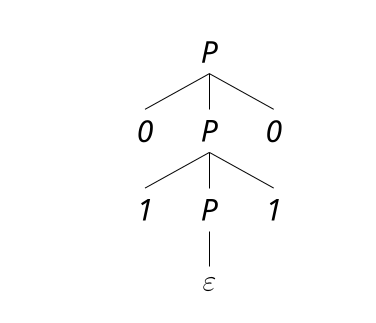
\includegraphics{example_1.1.1.png
}
%		\psframebox[linestyle=none,framesep=10pt]{%
%			\pstree{\LFTw{t}{\fontspec{Noto Sans}[Script=Latin]P}}{\pstree{\Tp[edge=none]}{%
%					\LFTw{t}{\fontspec{Noto Sans}[Script=Latin]0}
%					\pstree{\LFTw{t}{\fontspec{Noto Sans}[Script=Latin]P}}{\pstree{\Tp[edge=none]}{%
%							\LFTw{t}{\fontspec{Noto Sans}[Script=Latin]1}
%							\pstree{\LFTw{t}{\fontspec{Noto Sans}[Script=Latin]P}}{\pstree{\Tp[edge=none]}{%
%									\LFTw{t}{\fontspec{Noto Sans}[Script=Latin]$\varepsilon$}}}
%							\LFTw{t}{\fontspec{Noto Sans}[Script=Latin]1}}}
%					\LFTw{t}{\fontspec{Noto Sans}[Script=Latin]0}}}}
	\end{center}
\end{example}
\begin{example}
	Si ha:
	$$E\to I|\, E+E|\, E*E|\, (E)$$
	$$I\to a|\,b|\,Ia|\,Ib|\,I0|\,I1$$
	un albero sintattico per $a*(a+b00)$ può essere:
	\begin{center}
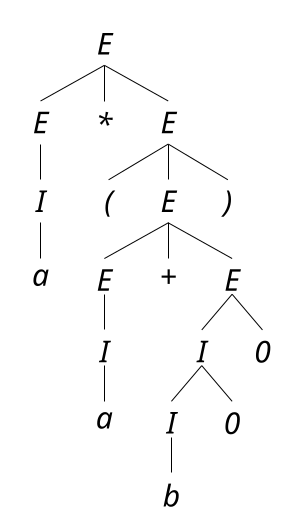
\includegraphics{example_1.1.2.png}
%		\psframebox[linestyle=none,framesep=10pt]{%
%			\pstree{\LFTw{t}{\fontspec{Noto Sans}[Script=Latin]E}}{\pstree{\Tp[edge=none]}{%
%					\pstree{\LFTw{t}{\fontspec{Noto Sans}[Script=Latin]E}}{\pstree{\Tp[edge=none]}{%
%							\pstree{\LFTw{t}{\fontspec{Noto Sans}[Script=Latin]I}}{\pstree{\Tp[edge=none]}{%
%									\LFTw{t}{\fontspec{Noto Sans}[Script=Latin]a}}}}}
%					\LFTw{t}{\fontspec{Noto Sans}[Script=Latin]*}
%					\pstree{\LFTw{t}{\fontspec{Noto Sans}[Script=Latin]E}}{\pstree{\Tp[edge=none]}{%
%							\LFTw{t}{\fontspec{Noto Sans}[Script=Latin](}
%								\pstree{\LFTw{t}{\fontspec{Noto Sans}[Script=Latin]E}}{\pstree{\Tp[edge=none]}{%
%										\pstree{\LFTw{t}{\fontspec{Noto Sans}[Script=Latin]E}}{\pstree{\Tp[edge=none]}{%
%												\pstree{\LFTw{t}{\fontspec{Noto Sans}[Script=Latin]I}}{\pstree{\Tp[edge=none]}{%
%														\LFTw{t}{\fontspec{Noto Sans}[Script=Latin]a}}}}}
%										\LFTw{t}{\fontspec{Noto Sans}[Script=Latin]+}
%										\pstree{\LFTw{t}{\fontspec{Noto Sans}[Script=Latin]E}}{\pstree{\Tp[edge=none]}{%
%												\pstree{\LFTw{t}{\fontspec{Noto Sans}[Script=Latin]I}}{\pstree{\Tp[edge=none]}{%
%														\pstree{\LFTw{t}{\fontspec{Noto Sans}[Script=Latin]I}}{\pstree{\Tp[edge=none]}{%
%																\LFTw{t}{\fontspec{Noto Sans}[Script=Latin]b}}}
%														\LFTw{t}{\fontspec{Noto Sans}[Script=Latin]0}}}
%												\LFTw{t}{\fontspec{Noto Sans}[Script=Latin]0}}}}}
%								\LFTw{t}{\fontspec{Noto Sans}[Script=Latin])}}}}}}
	\end{center}
\end{example}
\newpage
Data una CFG si ha che i seguenti cinque enunciati si equivalgono:
\begin{enumerate}
	\item la procedura di inferenza ricorsiva stailisce che una stringa $w$ di simboli terminali appartiene al linguaggio $L(A)$ con $A$ variabile
	\item $A\to ^*w$
	\item $A\to^*_{lm}w$
	\item $A\to^*_{rm}w$
	\item esiste un albero sintattico con radice $A$ e prodotto $w$
\end{enumerate}
queste 5 proposizioni si implicano l'uni l'altra:
\begin{center}
	\begin{tikzpicture}
		\node (top) at (0,0) {5};
		\node (a) at(-1,-0.5) {3};
		\node (b) at(0,-1) {4};
		\node (c) at(-2.0,-1.85) {2};
		\node (d) at(1.5,-2) {1};
		\draw [->] (top) -- (a);
		\draw [->] (top) -- (b);
		\draw [->] (a) -- (c);
		\draw [->] (b) -- (c);
		\draw [->] (c) -- (d);
		\draw [->] (d) -- (top);
	\end{tikzpicture}
\end{center}
vediamo qualche dimostrazione di implicazione tra queste proposizioni:
\begin{proof}[da 1 a 5]
	si procede per induzione:
	\begin{itemize}
		\item \textbf{caso base:} ho un livello solo (una sola riga), $\exists A\to w$:
					$$\overset{A}{\overset{\triangle}w}$$
		\item \textbf{caso passo:} suppongo vero per un numero di righe $\leq n$, lo dimsotro per $n+1$ righe:
					$$A\to X_1,X_2,...,X_k$$
					$$w=w_1,w_2,...,w_k$$
					ovvero, in meno di $n+1$ livelli:
					\begin{center}
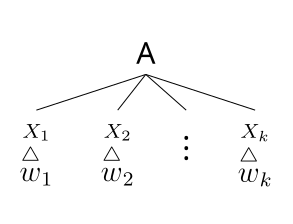
\includegraphics{caso_passo.png}
					% \psframebox[linestyle=none,framesep=10pt]{%
%				      \pstree{\LFTw{t}{\fontspec{Noto Sans}[Script=Latin]A}}{\pstree{\Tp[edge=none]}{%
%						      \LFTw{t}{\fontspec{Noto Sans}[Script=Latin]$\overset{X_1}{\overset{\triangle}w_1}$}
%						      \LFTw{t}{\fontspec{Noto Sans}[Script=Latin]$\overset{X_2}{\overset{\triangle}w_2}$}
%						      \LFTw{t}{\fontspec{Noto Sans}[Script=Latin]$\vdots$}
%						      \LFTw{t}{\fontspec{Noto Sans}[Script=Latin]$\overset{X_k}{\overset{\triangle}w_k}$}}}}
					\end{center}
	\end{itemize}
\end{proof}
\begin{proof}[da 5 a 3]
	procedo per induzione:
	\begin{itemize}
		\item \textbf{caso base (n=1): }$\exists A\to w\mbox{ quindi } A\to_{lm}w$, come prima si ha un solo livello:
					$$\overset{A}{\overset{\triangle}w}$$
		\item \textbf{caso passo: }suppongo che la proprierà valga per ogni albero di profondità minore uguale a $n$, dimostro che valga per gli alberi profondi $n+1$:
					$$A\to X_1,X_2,...,X_k$$
					$$w=w_1,w_2,...,w_k$$
					ovvero, in meno di $n+1$ livelli:
					\begin{center}
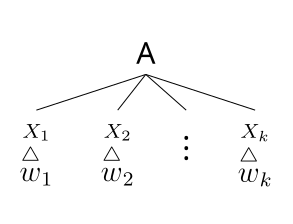
\includegraphics{caso_passo.png}
%			      \psframebox[linestyle=none,framesep=10pt]{%
%				      \pstree{\LFTw{t}{\fontspec{Noto Sans}[Script=Latin]A}}{\pstree{\Tp[edge=none]}{%
%						      \LFTw{t}{\fontspec{Noto Sans}[Script=Latin]$\overset{X_1}{\overset{\triangle}w_1}$}
%						      \LFTw{t}{\fontspec{Noto Sans}[Script=Latin]$\overset{X_2}{\overset{\triangle}w_2}$}
%						      \LFTw{t}{\fontspec{Noto Sans}[Script=Latin]$\vdots$}
%						      \LFTw{t}{\fontspec{Noto Sans}[Script=Latin]$\overset{X_k}{\overset{\triangle}w_k}$}}}}
					\end{center}
					$$A\to_{lm} X_1,X_2,...,X_k$$
					$$x_1\to^*_{lm}w_1 \mbox{ per ipotesi induttiva si ha un albero al più di n livelli}$$
					quindi:
					$$A\to_{lm}X_1,...,X_k\to^*_{lm}w_1,X_2,...,X_k\to^*_{lm}...\to^*_{lm}w_1,...,w_k=w$$
	\end{itemize}
	\begin{example}
		$$E\to I\to Ib\to ab$$
		$$\alpha E\beta\to\alpha I\beta\to \alpha Ib\beta\to \alpha ab\beta,\,\,\,\alpha,\beta\in(V\cup T)^*$$
	\end{example}
\end{proof}
\begin{example}
	Mostro l'esistenza di una derivazione sinistra dell'albero sintattico di $a*(a+b00)$:
	$$E\to^*_{lm}E*E\to^*_{lm}I*E\to^*_{lm}a*E\to^*_{lm}a*(E)\to^*_{lm}a*(E+E)\to^*_{lm}$$
	$$a*(I+E)\to^*_{lm}a*(a+E)\to^*_{lm}a*(a+I)\to^*_{lm}a+(a+I0)\to^*_{lm}a*(a+I00)\to^*_{lm}a*(a+b00)$$
\end{example}
\section{Grammatiche ambigue}
\begin{definition}
	Una grammatica è definita ambigua se esiste una stringa $w$ di terminali che ha più di un albero sintattico
\end{definition}
\begin{example}
	vediamo un esempio:
	\begin{enumerate}
		\item $E\to E+E\to E+E*E$
					ovvero:
					\begin{center}
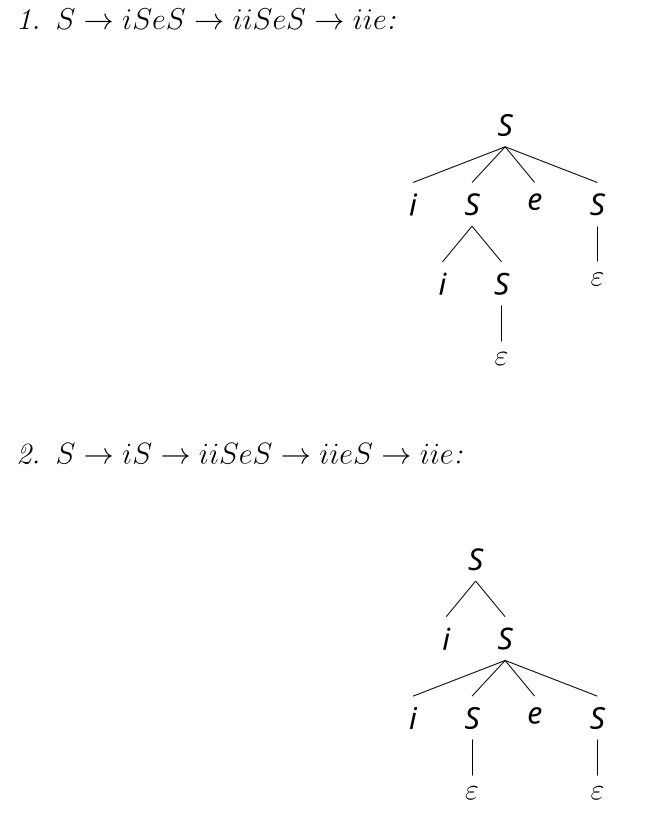
\includegraphics{ambigua1.png}
%			      \psframebox[linestyle=none,framesep=10pt]{%
%				      \pstree{\LFTw{t}{\fontspec{Noto Sans}[Script=Latin]E}}{\pstree{\Tp[edge=none]}{%
%						      \LFTw{t}{\fontspec{Noto Sans}[Script=Latin]E}
%						      \LFTw{t}{\fontspec{Noto Sans}[Script=Latin]+}
%						      \pstree{\LFTw{t}{\fontspec{Noto Sans}[Script=Latin]E}}{\pstree{\Tp[edge=none]}{%
%								      \LFTw{t}{\fontspec{Noto Sans}[Script=Latin]E}
%								      \LFTw{t}{\fontspec{Noto Sans}[Script=Latin]*}
%								      \LFTw{t}{\fontspec{Noto Sans}[Script=Latin]E}}}}}}
					\end{center}
		\item $E\to E*E\to E+E*E$
					ovvero:
					\begin{center}
%			      \psframebox[linestyle=none,framesep=10pt]{%
%				      \pstree{\LFTw{t}{\fontspec{Noto Sans}[Script=Latin]E}}{\pstree{\Tp[edge=none]}{%
%						      \pstree{\LFTw{t}{\fontspec{Noto Sans}[Script=Latin]E}}{\pstree{\Tp[edge=none]}{%
%								      \LFTw{t}{\fontspec{Noto Sans}[Script=Latin]E}
%								      \LFTw{t}{\fontspec{Noto Sans}[Script=Latin]+}
%								      \LFTw{t}{\fontspec{Noto Sans}[Script=Latin]E}}}
%						      \LFTw{t}{\fontspec{Noto Sans}[Script=Latin]*}
%						      \LFTw{t}{\fontspec{Noto Sans}[Script=Latin]E}}}}
					\end{center}
	\end{enumerate}
	si arriva a due stringhe uguali ma con alberi diversi. Introduciamo delle categorie sintatiche, dei vincoli alla produzione delle regole:
	\begin{enumerate}
		\item $E\to T|\, E+T$
		\item $T\to F|\, T+F$
		\item $F\to I|\, (E)$
		\item $I\to a|\,b|\,Ia|,Ib|\,I0|\,I1$
	\end{enumerate}
\end{example}
Possono esserci più derivazioni di una stringa ma l'importante è che non ci siano alberi sintattici diversi. Capire se una CFG è ambigua è un problema indecidibile
\begin{example}
	vediamo un esempio:
	$$S\to \varepsilon|\,SS|\, iS|\, iSeS$$
	con S=statement, i=if e e=else. Considero due derivazioni:
	\begin{enumerate}
		\item $S\to iSeS\to iiSeS\to iie$:
					\begin{center}
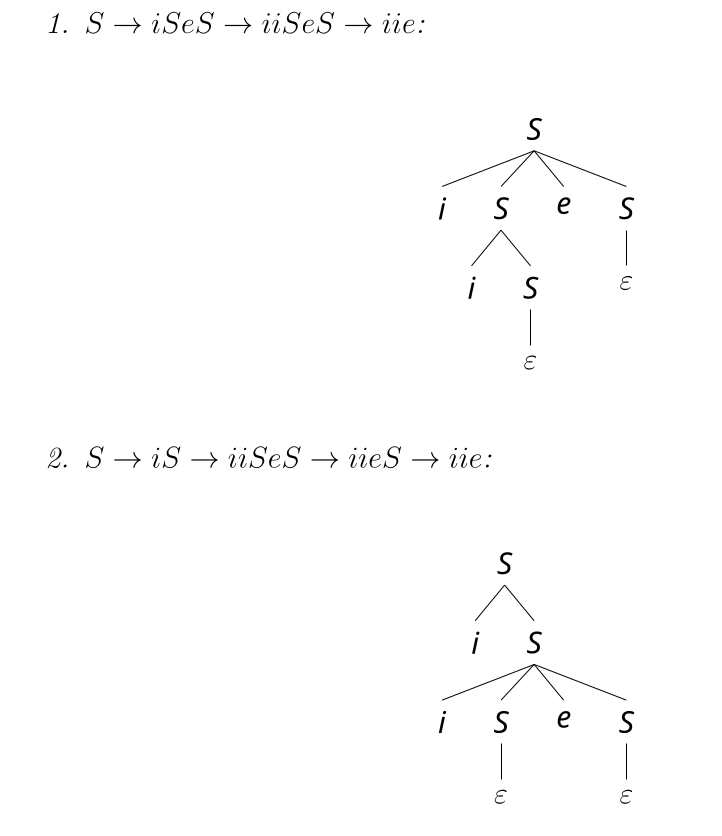
\includegraphics{ambigua2.png}

%			      \psframebox[linestyle=none,framesep=10pt]{%
%				      \pstree{\LFTw{t}{\fontspec{Noto Sans}[Script=Latin]S}}{\pstree{\Tp[edge=none]}{%
%						      \LFTw{t}{\fontspec{Noto Sans}[Script=Latin]i}
%						      \pstree{\LFTw{t}{\fontspec{Noto Sans}[Script=Latin]S}}{\pstree{\Tp[edge=none]}{%
%								      \LFTw{t}{\fontspec{Noto Sans}[Script=Latin]i}
%								      \pstree{\LFTw{t}{\fontspec{Noto Sans}[Script=Latin]S}}{\pstree{\Tp[edge=none]}{%
%										      \LFTw{t}{\fontspec{Noto Sans}[Script=Latin]$\varepsilon$}}}}}
%						      \LFTw{t}{\fontspec{Noto Sans}[Script=Latin]e}
%						      \pstree{\LFTw{t}{\fontspec{Noto Sans}[Script=Latin]S}}{\pstree{\Tp[edge=none]}{%
%								      \LFTw{t}{\fontspec{Noto Sans}[Script=Latin]$\varepsilon$}}}}}}\end{center}
%		\item $S\to iS\to iiSeS\to iieS\to iie$:
%		      \begin{center}
%
%			      \psframebox[linestyle=none,framesep=10pt]{%
%				      \pstree{\LFTw{t}{\fontspec{Noto Sans}[Script=Latin]S}}{\pstree{\Tp[edge=none]}{%
%						      \LFTw{t}{\fontspec{Noto Sans}[Script=Latin]i}
%						      \pstree{\LFTw{t}{\fontspec{Noto Sans}[Script=Latin]S}}{\pstree{\Tp[edge=none]}{%
%								      \LFTw{t}{\fontspec{Noto Sans}[Script=Latin]i}
%								      \pstree{\LFTw{t}{\fontspec{Noto Sans}[Script=Latin]S}}{\pstree{\Tp[edge=none]}{%
%										      \LFTw{t}{\fontspec{Noto Sans}[Script=Latin]$\varepsilon$}}}
%								      \LFTw{t}{\fontspec{Noto Sans}[Script=Latin]e}
%								      \pstree{\LFTw{t}{\fontspec{Noto Sans}[Script=Latin]S}}{\pstree{\Tp[edge=none]}{%
%										      \LFTw{t}{\fontspec{Noto Sans}[Script=Latin]$\varepsilon$}}}}}}}}
					\end{center}
	\end{enumerate}
	Si ha quindi una grammatica ambigua
\end{example}
\begin{theorem}
	Per ogni CFG, con $G=(V, T, P, S)$, per ogni stringa $w$ di terminali si ha che $w$ ha due alberi sintattici distinti sse ha due derivazioni sinistre da S distinte.\\
	Se la grammatica non è ambigua allora esiste un'unica derivazione sinistra da $S$
\end{theorem}
\subsubsection{Linguaggi inerentemente ambigui}
\begin{definition}
	Un linguaggio $L$ è inerentemente ambiguo se tutte le grammatiche CFG per tale linguaggio sono a loro volta ambigue
\end{definition}
\begin{example}
	Sia $L=\{a^nb^nc^md^m|\, n,m\geq 1\}\cup \{a^nbmnc^md^n|\, n,m\geq 1\}$\\
	si ha quindi un CFL formato dall'unione di due CFL. $L$ è inerentemente ambiguo e generato dalla seguente grammatica:
	\begin{itemize}
		\item $S\to AB|\,C$
		\item $A\to aAb|\,ab$
		\item $B\to cBd|\, cd$
		\item $C\to aCd|\, aDd$
		\item $D\to bDc|\, bc$
	\end{itemize}
	si possono avere due derivazioni:
	\begin{enumerate}
		\item $S\to_{lm}AB\to_{lm} aAbB\to_{lm} aabbB\to_{lm}aabbcBd\to_{lm}aabbccdd$
		\item $S\to_{lm} C\to_{lm} aCd\to_{lm}aaBdd\to_{lm}aabBcdd\to_{lm}aabbccdd$
	\end{enumerate}
	a generare problemi sono le stringhe con n=m perché possono essere prodotte in due modi diversi da entrambi i sottolinguaggi. Dato che l'intersezione tra i due sottolinguaggi non è buota si ha che $L$ è ambiguo
\end{example}
\section{Grammatiche Regolari}
Sono le grammatiche che generano i linguaggi regolari (quelli del terzo tipo) che sono casi particolari dei CFL.\\
Si ha la solita grammatica $G = (V, T, P, S)$ con però vincoli su $P$:
\begin{itemize}
	\item $\varepsilon$ si può ottenere solo con $S\to \varepsilon$
	\item le produzioni sono tutte lineari a destra ($A\to aA$ o $A\to a$) o a sinistra ($A\to Ba$ o $A\to a$)
\end{itemize}
\begin{example}
	$I\to a|\,b|\,Ia|\,Ib|\,I0|\,I1$ è una grammatica con le produzioni lineari a sinistra.\\
	Potremmo pensarlo a destra $I\to a|\,b|\,aI|\,bI|\,0I|\,1I$.\\
	Vediamo esempi di produzione con queste grammatiche:
	\begin{itemize}
		\item con $I\to a|\,b|\,Ia|\,Ib|\,I0|\,I1$ possiamo derivare $ab01b0$:
					$$I\to I0\to Ib0\to I1b0\to I01b0\to Ib01b0\to ab01b0$$
		\item con $I\to a|\,b|\,aI|\,bI|\,0I|\,1I$ invece non riusciamo a generare nulla:
					$$I\to 0I\to 0a$$
	\end{itemize}
	definisco quindi un'altra grammatica (con una nuova categoria sintattica):
	$$I\to aJ|\, bJ$$
	$$J\to a|\,b|\,aJ|\,bJ|\,0J|\,1J$$
	che però non mi permette di terminare le stringhe con 0 e 1, la modifico ancora otterdendo:
	$$I\to aJ|\, bJ$$
	$$J\to a|\,b|\,aJ|\,bJ|\,0J|\,1J|\,0|\,1$$
	e questo è il modo corretto per passare da lineare sinistra a lineare destra
\end{example}
\begin{example}
	Sia $G=(\{S\},\{0,1\},P,S)$ con $S\to \varepsilon|\,0|\,1|\,0S|\,1S$. Si ha quindi:
	$$L(G)=\{0,1\}^*$$
	si hanno comunque due proposizioni ridondanti, riducendo trovo:
	$$S\to \varepsilon|\, 0S|\,1S$$
	con solo produzioni lineari a destra. Con produzioni lineari a sinistra ottengo:
	$$S\to \varepsilon|\, S0|\,S1$$
\end{example}
\begin{example}
	Trovo una grammatica lineare destra e una sinistra per $L=\{a^nb^m|\,n,m\geq 0\}$:
	\begin{itemize}
		\item \textbf{lineare a destra:} si ha $G=(\{S,B\},\{a,b\},P,S)$ e quindi:
					$$S\to \varepsilon|\,aS|\,bB$$
					$$B\to bB|\,b$$
					ma non si possono generare stringhe di sole $b$, infatti:
					$$S\to aS\to abB\to abbB\to abbb$$
					ma aggiungere $\varepsilon$ a B \textbf{non è lecito}. posso però produrre la stessa stringa da due derivazioni diverse:
					$$S\to \varepsilon|\,aS|\,bB|\,b$$
					$$B\to bB|\,b$$
					che risulta quindi la nostra lineare a destra
		\item \textbf{lineare a sinistra:} si ha $G=(\{S,A\},\{a,b\},P,S)$ e quindi:
					$$S\to \varepsilon|\,Sb|\,Ab|\,a$$
					$$A\to Aa|\,a$$
	\end{itemize}
\end{example}
\begin{example}
	Trovo una grammatica lineare destra e una sinistra per $L=\{ab^ncd^me|\,n\geq 0\,,m> 0\}$:
	\begin{itemize}
		\item \textbf{lineare a destra:} si ha  si ha $G=(\{S,A,B,E\},\{a,b,c,d,e\},P,S)$ e quindi:
					$$S\to aA$$
					$$A\to bA|\,cB$$
					$$B\to dB|\, dE$$
					$$E\to e$$
		\item \textbf{lineare a sinistra:} si ha  si ha $G=(\{S,X,Y,Z\},\{a,b,c,d,e\},P,S)$ e quindi:
					$$S\to Xe$$
					$$A\to Xd|\,Yd$$
					$$B\to Zc$$
					$$E\to a|\,Zb$$
	\end{itemize}
	quindi se per esempio ho la stringa "ciao" si ha:
	\begin{itemize}
		\item \textbf{lineare a destra:}
					$$S\to Ao$$
					$$A\to Ba$$
					$$B\to Ei$$
					$$E\to c$$
		\item \textbf{lineare a sinistra:}
					$$S\to cA$$
					$$A\to iB$$
					$$B\to aE$$
					$$E\to o$$
	\end{itemize}
\end{example}
\begin{example}
	A partire da $G=(\{S,T\},\{0,1\},P,S)$ con:
	$$S\to\varepsilon|\,0S|\,1T$$
	$$T\to 0T|\,1S$$

	trovo come è fatto $L(G)$:
	$$L(G)=\{w\in\{0,1\}^*|\, w \mbox{ ha un numero di 1 pari}\}$$
\end{example}
\begin{example}
	fornire una grammatica regolare a destra e sinistra per:
	$$L=\{w\in\{0,1\}^*|\, w \mbox{ ha almeno uno 0 o almeno un 1}\}$$
	Si ah che tutte le stringhe tranne quella vuota ciontengono uno 0 o un 1
	quindi  $G=(\{S\},\{0,1\},P,S)$:
	\begin{itemize}
		\item \textbf{lineare a destra:}
					$$S\to 0|\,1|\,0S|\,1S$$
		\item \textbf{lineare a sinistra:}
					$$S\to 0|\,1|\,S0|\,S1$$
	\end{itemize}
\end{example}



Vediamo ora un esempio di \textit{Context Free Language (CFL)}, costruito a partire da una \textit{Context Free Grammar (CFG)}:
\begin{example}
	Sia $\Sigma=\{0, 1\}$ e $L_{pal}="stringhe\,\, palindrome\,\, binarie"$.
	Quindi, per esempio, $0110\in L,\,\, 11011\in L$ ma $10010\not\in L$. Si ha che $\varepsilon$, la stringa vuota, appartiene a $L$. Diamo una definizione ricorsiva:
	\begin{itemize}
		\item \textbf{base:} $\varepsilon,\, 0\,\ 1\in L_{pal}$
		\item \textbf{passo:} se $w$ è palindroma allora $0w0$ è palindromo e $1w1$ è palindromo
	\end{itemize}
	una variabile generica $S$ può sottostare alle \textit{regole di produzione} di una certa grammatica. In questo caso si ha uno dei seguenti:
	$$S\to\varepsilon,\, S\to 0,\, S\to 1,\, S\to 0S0,\, S\to 1S1$$
\end{example}


riprendiamo l'esempio sopra:
\begin{example}
	$$G_{pal}=(V=\{S\},\, T=\{0, 1\},\, P,\, S)$$
	con:
	$$P=\{S\to\varepsilon,\, S\to 0,\, S\to 1,\, S\to 0S0,\, S\to 1S1\}$$
	Si può ora costruire un algoritmo per creare una stringa palindroma a partire dalla grammatica $G$:
	$$\underbrace{S}_{\mbox{start}}\underbrace{\to}_{\mbox{applico una regola}} 1S1 \to 01S10\to \underbrace{01010}_{\mbox{sostituisco variabile}}$$

	con $S,\, 1S1\,\, e\,\, 01S10$ che sono \textit{forme sentenziali}. Posso così ottenere tutte le possibili stringhe. Esiste anche una forma abbreviata:
	$$S\to \varepsilon|o|1|0S0|1S1$$
	Non si fanno sostituzioni in parallelo, prima una $S$ e poi un'altra
\end{example}


\section{Automi a Pila}\label{sec:automi-pila}

	Si introduce un nuovo tipo di automa, il PDA (push down automata) che può essere pensato come un $\varepsilon-NFA$ col supporto di una pila (stack):
	\begin{center}
	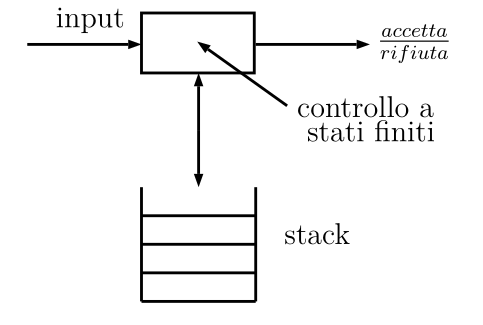
\includegraphics{2025-01-16_14-59.png}
		% \psscalebox{1.0 1.0} % Change this value to rescale the drawing.
		% {
		% 	\begin{pspicture}(0,-2.04)(5.83,2.04)
		% 		\psframe[linecolor=black, linewidth=0.04, dimen=outer](3.2,2.04)(1.58,1.16)
		% 		\psline[linecolor=black, linewidth=0.04, arrowsize=0.05291667cm 2.0,arrowlength=1.4,arrowinset=0.0]{->}(0.0,1.58)(1.6,1.58)
		% 		\psline[linecolor=black, linewidth=0.04, arrowsize=0.05291667cm 2.0,arrowlength=1.4,arrowinset=0.0]{->}(3.2,1.58)(4.8,1.58)
		% 		\psline[linecolor=black, linewidth=0.04, arrowsize=0.05291667cm 2.0,arrowlength=1.4,arrowinset=0.0]{->}(2.4,0.38)(2.4,-0.42)
		% 		\psline[linecolor=black, linewidth=0.04, arrowsize=0.05291667cm 2.0,arrowlength=1.4,arrowinset=0.0]{->}(2.4,0.38)(2.4,1.18)
		% 		\psline[linecolor=black, linewidth=0.04](1.6,-0.42)(1.6,-2.02)
		% 		\psline[linecolor=black, linewidth=0.04](3.2,-2.02)(1.6,-2.02)
		% 		\psline[linecolor=black, linewidth=0.04](3.2,-2.02)(3.2,-0.42)
		% 		\psline[linecolor=black, linewidth=0.04](1.6,-0.82)(3.2,-0.82)
		% 		\psline[linecolor=black, linewidth=0.04](1.6,-1.22)(3.2,-1.22)
		% 		\psline[linecolor=black, linewidth=0.04](1.6,-1.62)(3.2,-1.62)
		% 		\rput[bl](4.9,1.32){$\frac{accetta}{rifiuta}$}
		% 		\rput[bl](0.4,1.74){input}
		% 		\rput[bl](3.78,0.22){ stati finiti}
		% 		\rput[bl](3.6,-1.22){stack}
		% 		\psline[linecolor=black, linewidth=0.04, arrowsize=0.05291667cm 2.0,arrowlength=1.4,arrowinset=0.0]{->}(3.64,0.72)(2.38,1.62)
		% 		\rput[bl](3.78,0.56){controllo a}
		% 	\end{pspicture}
		% }
	Tikz
	\end{center}
	e viene definito un PDA $P$ come:
	$$P=(Q,\Sigma,\Gamma,\delta,q_0,z_0,F)$$
	con;
	\begin{itemize}
		\item $Q$: insieme finito e non vuoto di stati
		\item $\Sigma$: alfabeto di simboli di input
		\item $\Gamma$: alfabeto di simboli di stack
		\item $q_0\in Q$: stato iniziale
		\item $z_0\in \Gamma\backslash \Sigma$: simbolo iniziale dello stack
		\item $F\in Q$: insieme degli stati accettanti o finali
	\end{itemize}
	si ha che:
	$$\delta:Q\times(\Sigma\cup\{\varepsilon\}\times \Gamma\to 2^{Q\times \Gamma^*}$$
	quindi:
	$$\delta(q_0,a,X)=\{(p_1,X_1),(p_2,X_2),...\}\,insieme\,\,\,finito\,\,p_i\in Q\,\,X_i\in \Gamma^*$$
	si hanno dei casi particolari:
	\begin{itemize}
		\item lo stato $p$ potrebbe coincidere con $Q$ e si avrebbe un cappio
		\item se $\Gamma=\varepsilon$ si ha il pop di $X$ dallo stack
		\item se $\Gamma=X$ si lascia lo stack invariato
		\item se $\Gamma=Y\neq X$ si ha la sostituzione di $X$ con $Y$ in cima allo stack
		\item se $\Gamma$ è una stringa di simboli si ha il la rimozione di $X$ dallo stack e l'aggiunta a uno a uno dei simboli nello stack
	\end{itemize}
	\newpage
	\begin{example}
		Trovo PDA per il linguaggio delle stringhe binarie  palindrome di lunghezza pari: $L=\{ww^R|w\in\{0,1\}^*\}$. Con $R$ che indica rovesciato\\
		Si ha la CFG $G=(\{P\},\{0,1\},Prod,P)$ tale che:
		$$P\to 0P0|1P1|\varepsilon$$
		si hanno quindi tre stati:
		\begin{itemize}
			\item $q_0$ che è quello iniziale che legge $w$ e spinge i dati sullo stack
			\item $q_1$ che letta $w$ legge i simboli di $wR$ e li confronta con quelli dello stack
			\item $q_2$ sarà la stringa accettata
		\end{itemize}
		descriviamo formalmente l'automa con la funzione di transizione $\delta$.
		PDA $P=(\{q_0,q_1,q_2\},\{0,1\}, \{o,1,z_0\},\delta,q_0,z_0,\{q_2\})$
		ovvero:
		$$\delta(q_0,0,z_0)=\{(q_0,1z_0)\}$$
		$$\delta(q_0,1,z_0)=\{(q_0,0z_0)\}$$
		$$\delta(q_0,0,0)=\{(q_0,00)\}$$
		$$\delta(q_0,0,1)=\{(q_0,01)\}$$
		$$\delta(q_0,1,0)=\{(q_0,10)\}$$
		$$\delta(q_0,1,1)=\{(q_0,11)\}$$
		$$\delta(q_0,\varepsilon,z_0)=\{(q_0,z_0)\}$$
		$$\delta(q_0,\varepsilon,0)=\{(q_0,0)\}$$
		$$\delta(q_0,\varepsilon,1)=\{(q_0,1)\}$$
		$$\delta(q_1,0,0)=\{(q_1,\varepsilon)\}$$
		$$\delta(q_2,1,1)=\{(q_1,\varepsilon)\}$$
		$$\delta(q_2,\varepsilon,z_0)=\{(q_2,0z_0)\}$$
		\newpage
		otteniamo il seguente PDA:
		\begin{center}
			\begin{tikzpicture}[shorten >=1pt,node distance=3cm,on grid,auto]
				\node[state, initial] (q_0) {$q_0$};
				\node[state] (q_1) [right=of q_0] {$q_1$};
				\node[state, accepting] (q_2) [right =of q_1] {$q_2$};
				\path[->]
				(q_0) edge node [align=center] {$\varepsilon,0/0$\\$\varepsilon,1/1$\\$\varepsilon,z_0/z_0$} (q_1)
				edge [loop below] node [align=center] {$0,z_0/0z_0$\\$1,z_0/1z_0$\\$0,0/00$\\$0,1/01$\\$1,0/10$\\$1,1/11$} ()
				(q_1) edge [loop below] node [align=center] {$0,0/\varepsilon$\\$1,1/\varepsilon$} ()
				edge  node [align=center] {$\varepsilon,z_0/z_0$} (q_2);
			\end{tikzpicture}
		\end{center}
		e si definisce questa notazione per gli archi:
		$$(p,\alpha)\in\delta(q,a,X)$$
		\begin{center}
			\begin{tikzpicture}[shorten >=1pt,node distance=3cm,on grid,auto]
				\node[state, initial] (q_0) {$q_0$};
				\node[state] (q_1) [right=of q_0] {$q_1$};
				\path[->]
				(q_0) edge node [align=center] {$a,X/\alpha$} (q_1);
			\end{tikzpicture}
		\end{center}
	\end{example}
	analizziamo meglio i PDA. Si ha che la \textbf{descrizione istantanea (ID)} di un PDA è una tripla:
	$$ID:(q,w,\gamma)$$
	con $q\in Q$ stato attuale $w\in\Sigma^*$ input rimanente e $\gamma\in\Gamma^*$ contenuto attuale dello stack.\\
	Definiamo ora il concetto di \textbf{mossa in un passo}
	dato $P=(Q,\Sigma,\Gamma,\delta,q_0,z_0,F)$ la mossa è una relazione $\vdash_p$:
	$$(p,\alpha)\in\delta(q,a,X)\,\,allora\,\,\forall w\in\Sigma^*\,\,e\,\, \forall\beta\in\Gamma^*\to (q,aw,X\beta)\vdash(p,w,\alpha\beta$$
	e
	$$(p,\alpha)\in\delta(q,\varepsilon,X)\,\,allora\,\,\forall w\in\Sigma^*\,\,e\,\, \forall\beta\in\Gamma^*\to (q,w,X\beta)\vdash(p,w,\alpha\beta)$$
	\newpage
	ora possiamo anche definire la relazione con 0 o più mosse
	in forma induttiva $\stackrel{*}{\vdash_p}$:
	\begin{itemize}
		\item \textbf{caso base:} $\forall ID\,\,I, I \stackrel{*}{\vdash} I$
		\item \textbf{caso passo:} $I \stackrel{*}{\vdash} J$ se $\exists ID\,\,K$ tale che $ I\vdash K \,\,e\,\, K \stackrel{*}{\vdash} J$
	\end{itemize}
	vediamo un esempio con un PDA che accetta $ww^R|\,w\in\{0,1\}^*$:
	\begin{center}
		\begin{tikzpicture}[shorten >=1pt,node distance=3cm,on grid,auto]
			\node[state, initial] (q_0) {$q_0$};
			\node[state] (q_1) [right=of q_0] {$q_1$};
			\node[state, accepting] (q_2) [right =of q_1] {$q_2$};
			\path[->]
			(q_0) edge node [align=center] {$\varepsilon,0/0$\\$\varepsilon,1/1$\\$\varepsilon,z_0/z_0$} (q_1)
			edge [loop below] node [align=center] {$0,z_0/0z_0$\\$1,z_0/1z_0$\\$0,0/00$\\$0,1/01$\\$1,0/10$\\$1,1/11$} ()
			(q_1) edge [loop below] node [align=center] {$0,0/\varepsilon$\\$1,1/\varepsilon$} ()
			edge  node [align=center] {$\varepsilon,z_0/z_0$} (q_2);
		\end{tikzpicture}
	\end{center}
	e prendiamo la stringa $1111$:\\
	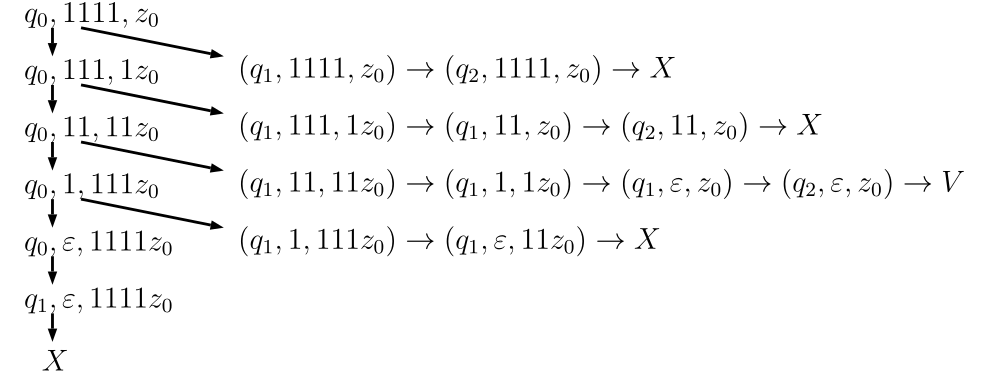
\includegraphics{2025-01-16_15-01.png}
	% \\
	% \psscalebox{1.0 1.0} % Change this value to rescale the drawing.
	% {
	% 	\begin{pspicture}(0,-2.51)(3.08,2.51)
	% 		\rput[bl](0.0,2.29){$q_0,1111,z_0$}
	% 		\rput[bl](0.0,1.49){$q_0,111,1z_0$}
	% 		\rput[bl](0.0,0.69){$q_0,11,11z_0$}
	% 		\rput[bl](0.0,-0.11){$q_0,1,111z_0$}
	% 		\rput[bl](0.0,-0.91){$q_0,\varepsilon,1111z_0$}
	% 		\rput[bl](0.0,-1.71){$q_1,\varepsilon,1111z_0$}
	% 		\rput[bl](0.25,-2.51){$X$}
	% 		\rput[bl](3.0,1.49){$(q_1,1111,z_0)\to(q_2,1111,z_0)\to X$}
	% 		\rput[bl](3.0,0.69){$(q_1,111,1z_0)\to (q_1,11,z_0)\to(q_2,11,z_0)\to X$}
	% 		\rput[bl](3.0,-0.11){$(q_1,11,11z_0)\to(q_1,1,1z_0)\to(q_1,\varepsilon,z_0)\to(q_2,\varepsilon,z_0)\to V$}
	% 		\rput[bl](3.0,-0.91){$(q_1,1,111z_0)\to(q_1,\varepsilon,11z_0)\to X$}
	% 		\psline[linecolor=black, linewidth=0.04, arrowsize=0.05291667cm 2.0,arrowlength=1.4,arrowinset=0.0]{->}(0.4,2.29)(0.4,1.89)
	% 		\psline[linecolor=black, linewidth=0.04, arrowsize=0.05291667cm 2.0,arrowlength=1.4,arrowinset=0.0]{->}(0.4,1.49)(0.4,1.09)
	% 		\psline[linecolor=black, linewidth=0.04, arrowsize=0.05291667cm 2.0,arrowlength=1.4,arrowinset=0.0]{->}(0.4,0.69)(0.4,0.29)
	% 		\psline[linecolor=black, linewidth=0.04, arrowsize=0.05291667cm 2.0,arrowlength=1.4,arrowinset=0.0]{->}(0.4,-0.11)(0.4,-0.51)
	% 		\psline[linecolor=black, linewidth=0.04, arrowsize=0.05291667cm 2.0,arrowlength=1.4,arrowinset=0.0]{->}(0.4,-0.91)(0.4,-1.31)
	% 		\psline[linecolor=black, linewidth=0.04, arrowsize=0.05291667cm 2.0,arrowlength=1.4,arrowinset=0.0]{->}(0.4,-1.71)(0.4,-2.11)
	% 		\psline[linecolor=black, linewidth=0.04, arrowsize=0.05291667cm 2.0,arrowlength=1.4,arrowinset=0.0]{->}(0.8,1.49)(2.8,1.09)
	% 		\psline[linecolor=black, linewidth=0.04, arrowsize=0.05291667cm 2.0,arrowlength=1.4,arrowinset=0.0]{->}(0.8,2.29)(2.8,1.89)
	% 		\psline[linecolor=black, linewidth=0.04, arrowsize=0.05291667cm 2.0,arrowlength=1.4,arrowinset=0.0]{->}(0.8,0.69)(2.8,0.29)
	% 		\psline[linecolor=black, linewidth=0.04, arrowsize=0.05291667cm 2.0,arrowlength=1.4,arrowinset=0.0]{->}(0.8,-0.11)(2.8,-0.51)
	% 	\end{pspicture}
	% }
	\\
	chiamiamo \textbf{computazione }una sequenza di mosse, non necessariamente di successo. Si hanno alcune proprietà:
	\begin{itemize}
		\item se una se una sequenza di ID è lecita per un PDA P allora è lecita anche la sequenza di Id ottenuta concatenando $w\in\Sigma^*$ in ogni ID
		\item se una se una sequenza di ID è lecita per un PDA P e resta una coda di input non consumata allora posso rimuovere tale coda in ogni ID e ottenere un'altra sequenza lecita
		\item se una se una sequenza di ID è lecita per un PDA P allora  è lecita la sequenza ottenuta aggiungendo $\gamma\in\Gamma^*$ in coda alla terza sequenza di ogni ID
	\end{itemize}
	del resto però:
	$$(q,Xw,\alpha\gamma) \stackrel{*}{\vdash_p} (p,Yw,\beta\gamma)\not\to (q,X,\alpha) \stackrel{*}{\vdash}(p,y,\beta),\,\,x,w,y\in\Sigma^*\,\,\alpha,\beta,\gamma\in\Gamma^*$$
	per queste proprietà valgono i seguenti teoremi:
	\begin{theorem}
		per la seconda:
		Se $P=(Q,\Sigma,\Gamma,\delta,q_0,z_0,F)$ è un PDA e $(q,Xw,\alpha) \stackrel{*}{\vdash_p} (p,Yw,\beta)$ allora vale anche:
		$$(q,X,\alpha) \stackrel{*}{\vdash_p} (p,Y,\beta)$$
	\end{theorem}
	\begin{theorem}
		per la prima e la terza:
		Se $P=(Q,\Sigma,\Gamma,\delta,q_0,z_0,F)$ è un PDA e $(q,X,\alpha) \vdash_p^* (p,Y,\beta)$ allora:
		$$\forall\gamma\in\Gamma^*\,\,\,vale\,\,\,anche\,\,\,(q,Xw,\alpha\gamma) \vdash_p^* (p,Yw,\beta\gamma)$$
	\end{theorem}
	Si definiscono due modalità di accettazione per i PDA:
	\begin{enumerate}
		\item \textbf{per stato finale:} sia $P=(Q,\Sigma,\Gamma,\delta,q_0,z_0,F)$ si ha che:
		      $$L(P)=\{w\in\Sigma^*|\,(q_0,w,z_0) \vdash_p^* (q,\varepsilon,\alpha)\}$$
		      con $q\in F$ e $\forall \alpha\in \Gamma^*$
		\item \textbf{per stack vuoto:} sia $P=(Q,\Sigma,\Gamma,\delta,q_0,z_0,F)$ si ha che:
		      $$N(P)=\{w\in\Sigma^*|\,(q_0,w,z_0) \vdash_p^* (q,\varepsilon,\varepsilon)\}$$
		      con $q\in Q$ e in questo caso l'insieme degli stati finali $F$ non ha alcuna influenza
	\end{enumerate}
	In realtà si ha che la classe di linguaggi accettati dai PDA per stato finale è uguale a quella per stack vuoto, anche se passare da un tipo all'altro di PDA è complesso. SI ha il seguente teorema per la trasformazione:
	\begin{theorem}
		se $L=N(P_N)$ per un PDA  $P_N=(Q,\Sigma,\Gamma,\delta,q_0,z_0,F)$ allora $\exists \,\,PDA\,\,P_F\,\,\,tale\,\,\,che\,\,\,L=L(P_F)$
	\end{theorem}
	\begin{proof}
		Sia $x_0\in\Gamma$, che indica la fine dello stack di $P_F$. Si ha:
		$$\delta(p_0,\varepsilon,x_0)=\{(q_0,z_0x_0\}$$
		e:
		$$\forall q\in Q,\,\forall a\in\Sigma\cup\{\varepsilon\},,\forall y\in\Sigma:\,\,\delta_F(q,a,y)\mbox{ contiene tutte le coppie di }\delta_N(q,a,y)$$
		$$\forall q\in Q,\delta_F(q,\varepsilon,x_0)=\{(P_F,\varepsilon)\}$$
		quindi graficamente:

		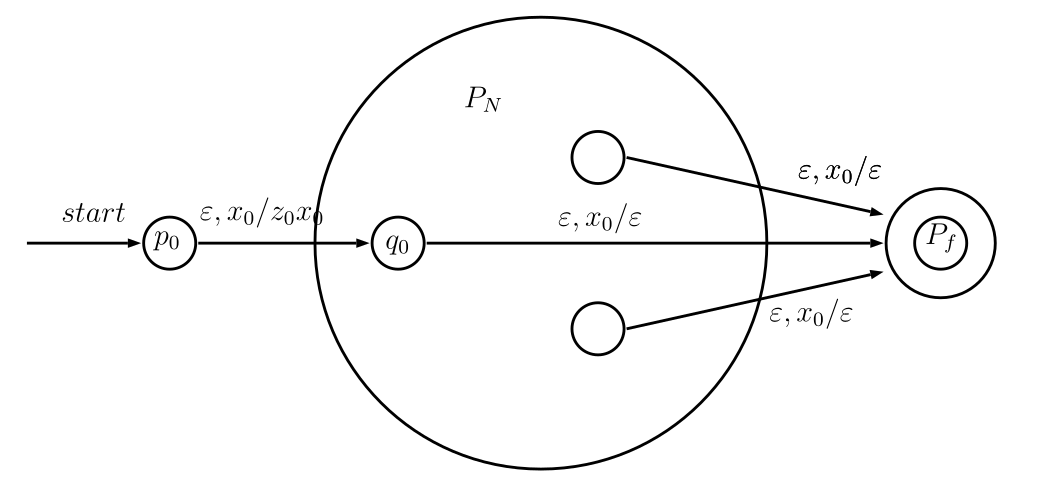
\includegraphics{2025-01-16_15-03.png}
		Bisogna dimostrare che effettivamente $w\in L(P_F)\longleftrightarrow\in N(P_N)$.\\
		se $w\in N(P_N)$ $\exists$ una sequenza di $ID\,\,\,(q_0,w,z_0)\vdash_{P_N}^*(q,\varepsilon,\varepsilon)$ per un qualche $q\in Q$:
		$$(q_0,w,z_0x_0)\vdash_{P_N}^*(q,\varepsilon,x_0)$$
		inoltre:
		$$(q_0,w,z_0x_0)\vdash_{P_F}^*(q,\varepsilon,x_0)$$
		e quindi:
		$$(p_0,w,x_0)\vdash_{P_F}(q_0,w,z_0x_0)\vdash_{P_F}^*(q,\varepsilon,x_0)\vdash_{P_F}(P_F,\varepsilon,\varepsilon)$$
		solo se togliendo il primo e l'ultimo passo di $P_F$ ripercorro all'indietro quanto scritto sopra.
	\end{proof}
	\begin{example}
		trasformazione da accettante per stack vuoto a accettante per stato finale. Siano:
		$$\Sigma=\{i,e\}$$
		$$P_n=(\{q\}, \{i,e\},\{Z\},\delta_M,q,Z)$$
		$$\delta_N(q,i,Z)=\{(q,ZZ)\}$$
		$$\delta_N(q,e,Z)=\{(q,\varepsilon)\}$$
		quindi:
		\begin{center}
			\begin{tikzpicture}[shorten >=1pt,node distance=3cm,on grid,auto]
				\node[state, initial] (q_0) {$q$};
				\path[->]
				(q_0) edge [loop above] node [align=center] {$i,Z/ZZ$\\$e,Z/\varepsilon$} ();
			\end{tikzpicture}
		\end{center}
		quindi inseriamo una $Z$ quando leggiamo $i$ e ne rimuoviamo una se leggiamo $e$ e si parte con una $Z$ nello stack.\\
		Costruisco ora il PDA $P_F$ che accetta lo stesso linguaggio ma per stato finale, introduco lo stato iniziale $p$ e quello  accettante $r$, uso $x_0$ come segnale della fine dello stack:
		\begin{center}
			\begin{tikzpicture}[shorten >=1pt,node distance=3cm,on grid,auto]
				\node[state, initial] (q_0) {$p$};
				\node[state] (q_1) [right=of q_0] {$q$};
				\node[state, accepting] (q_2) [right =of q_1] {$r$} ;
				\path[->]
				(q_0) edge  node [align=center] {$\varepsilon x_0/zx_0$} (q_1)
				(q_1) edge node {$\varepsilon,x_0/\varepsilon$} (q_2)
				edge [loop above] node [align=center] {$i,Z/ZZ$\\$e,Z/\varepsilon$} ();
			\end{tikzpicture}
		\end{center}
		e si ha formalmente:
		$$P_F=(\{p,q,r\}, \{i,e\},\{Z,x_0\},\delta_F,p,x_0,\{r\})$$
		con $\delta_F$ che rappresenta le seguenti quattro regole:
		\begin{enumerate}
			\item $\delta_F(p,\varepsilon,x_0)=\{(q,Zx_0)\}$ regola che fa partire $P_F$ con $x_o$ come segnalatore dello stack
			\item $\delta_F(p,i,Z)=\{(q,ZZ)\}$ regola che inserisce $Z$ quando si ha $i$ simulando $P_N$
			\item $\delta_F(p,e,Z)=\{(q,Z\varepsilon)\}$ regola che rimuove $Z$ quando si ha $e$ simulando $P_N$
			\item $\delta_F(p,e,x_0)=\{(r,\varepsilon)\}$ regola che permette a $P_F$ di accettare quando $P_N$ esaurisce lo stack
		\end{enumerate}
	\end{example}
	Si può anche effettuare la trasformazione inversa:
	\begin{theorem}
		Sia $P_F=(Q,\Sigma,\Gamma,\delta_f,q_0,Z_0,F)$.\\
		Si aggiunge una transizione $\varepsilon$  a un nuovo stato $p$ da ogni accettante di $P_F$. quando si ha $p$ $P_N$ svuota lo stack senza consumare input. Quindi se $P:F$ entra in uno stato accettante dopo aver consumato l'input $w$, $P_N$ svuota lo stack dopo aver consumato $w$. Per evitare che si svuoti lo stack per una stringa non accettata uso $x_0$ per indicare il fondo dello stack. Il nuovo $P_N$ parte da $p_0$ che ha il solo scopo di inserire il simbolo iniziale di $P_F$ e passare al suo stato iniziale. Si ottiene quindi:
		\begin{center}
		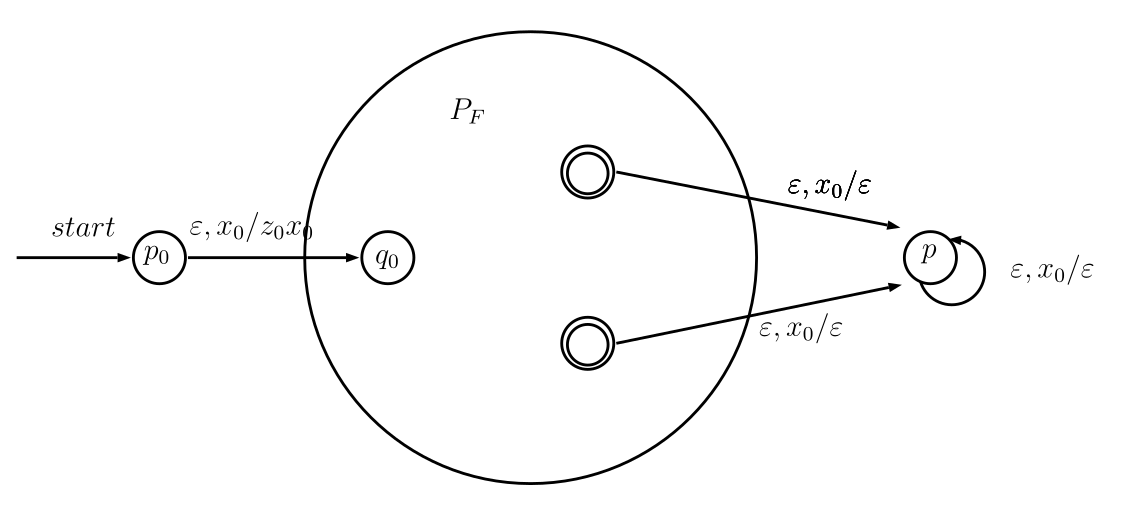
\includegraphics{2025-01-16_15-04.png}
		\end{center}
		e si ha formalmente:
		$$P_F=(Q\cup\{p_0,p\}, \Sigma,\Gamma\cup\{x_0\},\delta_N,p_0,x_0)$$
		dove $\delta_N$ è così definita:
		\begin{enumerate}
			\item $\delta_N(p_0,\varepsilon,x_0)=\{(q_0,Z_0x_0)\}$ inserisce il simbolo iniziale di $P_F$ nello stack e va allo stato iniziale di $P_F$
			\item $\forall q\in Q$ ogni simbolo di input $a\in\Sigma$, compreso l'input vuoto, e $\forall y\in \Gamma$, $\delta_N(q,a,y)$  contiene tutte le coppie di $\delta_F(q,a,y)$. Quindi $P_N$ simula $P_F$
			\item per tutti gli stati accettanti $q\in F$ e i simboli di stack $y\in\Gamma$, compreso $x_0$, si ha che $\delta_N(q,\varepsilon,y)$ contiene $(p,\varepsilon)$, quindi ogni volta che $P_F$ accetta $P_N$ inizia scaricare lo stack senza consumare ulteriori input
			\item per tutti  i simboli di stack $y\in\Gamma$, compreso $x_0$, si ha che $\delta_N(q,\varepsilon,y)=\{(p,\varepsilon)\}$, quindi giunti allo stato $p$, ovvero quando $P_F$ ha accettato, $P_N$ elimina ogni simbolo nel suo stack fino a svuotarlo
		\end{enumerate}
		inoltre formalmente voglio dimostrare che:
		$$w\in L(P_F)\to w\in N(P_N)$$
		e quindi ho le seguenti mosse:
		$$(q_0,w,z_0)\vdash_{P_F}^*(q,\varepsilon,\alpha)\,\,q\in F,\,\,\alpha\in\Gamma^*$$
		$$(p_o,w,x_0)\vdash(q_0,w,z_0x_0)\vdash_{P_N}^*(q,\varepsilon,\alpha,x_0)\vdash_{P_N}^*(p,\varepsilon,\varepsilon)$$
	\end{theorem}
	\begin{example}
		si ha una CFG $G=(\{i,e\},\{a,b,0,1,*,+,(,)\},P,E)$
		con:
		$$P:I\to a|b|Ia|Ib|I0|I1$$
		$$\,\,E\to E+E|E*E|(E)$$
		si ha il PDA $P_G=(\{q\},\Sigma,\Sigma\cup\{i,e\},\delta,q,E)$:
		\begin{center}
			\begin{tikzpicture}[shorten >=1pt,node distance=3cm,on grid,auto]
				\node[state, initial] (q_0) {$q$};
				\path[->]
				(q_0) edge [loop above] node [align=center] {$\mbox{ }$} ();
			\end{tikzpicture}
		\end{center}
		si ha quindi:
		$$\delta(q,\varepsilon, i)=\{(q,a),(q,b),(q,Ia),(q,Ib),(q,I0),(q,I1)\}$$
		$$\delta(q,\varepsilon, E)=\{(q,I),(q,E+E),(q,E*E),(q,I(E))\}$$
		$$\delta(q,a,a)=\{(q,\varepsilon)\}$$
		$$\delta(q,b,b)=\{(q,\varepsilon)\}$$
		$$\cdots=\{(q,\varepsilon)\}$$
		quindi si ha:
		$$E\to E+E\to i+E\to a+(E)\to a+(i)\to a+(i0)\to a+(b0)$$
		$$(q, a+(b0),E)\vdash (q, a+(b0),E+E)\vdash (q, a+(b0),i+E)\vdash (q, a+(b0),a+E)$$
		$$\vdash (q, +(b0),+E)\vdash (q, (b0),E)\vdash (q, (b0),(E))\vdash (q, b0),E))$$
		$$\vdash (q, b0),i))\vdash (q, b0),i0))\vdash (q, b0),b0)\vdash (q, 0),0))$$
		$$\vdash (q, ),))\vdash (q, \varepsilon,\varepsilon)$$
	\end{example}
	questo esempio è generalizzabile ad ogni CFG


	\begin{theorem}
		sia $G=(V,T,P,S)$ una CFG:
		$$\exists\,\, PDA\,\,Q=(\{q\},T,V\cup T,\delta,q,S)\mbox{ tale che }N(Q)=L(G)$$
		$$\forall A\in V\,\,\delta(q,\varepsilon,A)=\{(q,\beta)|\,A\to B\mbox{ e' una produzione di G}\}$$
		$$\forall a\in T\,\,\delta(q,a,a)=\{(a,\varepsilon)\}$$
	\end{theorem}
	Questo dimostra che ogni CFL può essere accettato da un PDA accettante per stack vuoto. Per il teorema visto in precedenza, posso sempre costruire un altro PDA accettante per stati finale. I PDA accettano tutti e soli i linguaggi CF. Mostrare che accettano solo linguaggi di tipo 2 è complicato.\\
	Un tipo di PDA interessante, soprattutto per i parse, è il PDA deterministico, il \textbf{DPDA}.\\
	Un PDA $P=(Q,\Sigma,\Gamma,\delta,q_0,z_0,F)$ è deterministico se:
	\begin{enumerate}
		\item $|\delta(q,a,x)|\leq 1$ $\forall q\in Q,\forall a\in\Sigma\cup\{\varepsilon\},\forall x\in \Gamma$
		\item se $|\delta(q,a,x)|\neq 0$ per qualche $a\in \Sigma$ allora $|\delta(q,\varepsilon,x)|=0$
	\end{enumerate}
	\begin{example}
		abbiamo il linguaggio $L_{wcw^R}=\{wcw^R|\,w\in\{0,1\}^*\}$\\
		Gli automi a pila deterministici non riconosco tutti i CFL, ma solo una classe strettamente più piccola. Ad esempio non potrebbero riconoscere il linguaggio delle palindrome senza "il segnalibro" c. SI ha quindi:
		\begin{center}
			\begin{tikzpicture}[shorten >=1pt,node distance=3cm,on grid,auto]
				\node[state, initial] (q_0) {$q_0$};
				\node[state] (q_1) [right=of q_0] {$q_1$};
				\node[state, accepting] (q_2) [right =of q_1] {$q_2$} ;
				\path[->]
				(q_0) edge [loop above] node [align=center] {$0,z_0/0z_0$\\$1,z_0/1z_0$\\$0,0/00$\\$0,1/01$\\$1,0/10$\\$1,1/11$} ()
				edge node [align=center] {$c,z_0/0z_0$\\$c,0/0$\\$c,1/1$} (q_1)
				(q_1) edge node {$\varepsilon,z_0/z_0$} (q_2)
				edge [loop above] node [align=center] {$0,0/\varepsilon$\\$1,1/\varepsilon$} ();
			\end{tikzpicture}
		\end{center}
		quindi:
		\begin{center}
		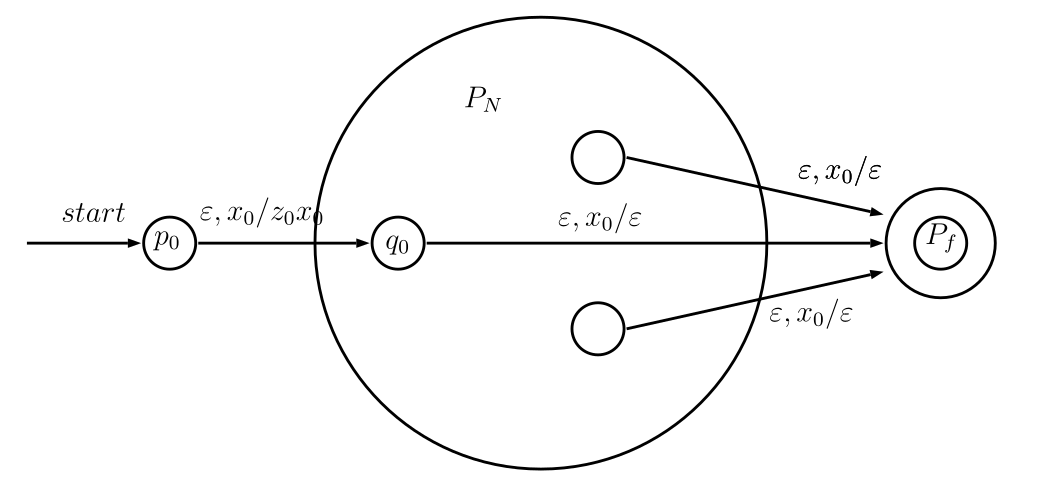
\includegraphics{2025-01-16_15-03.png}
			% \psscalebox{1.0 1.0} % Change this value to rescale the drawing.
			% {
			% 	\begin{pspicture}(0,-2.0)(7.6,2.0)
			% 		\psframe[linecolor=black, linewidth=0.04, dimen=outer](7.6,2.0)(0.0,-2.0)
			% 		\psframe[linecolor=black, linewidth=0.04, dimen=outer](4.8,0.8)(0.8,-1.2)
			% 		\psframe[linecolor=black, linewidth=0.04, dimen=outer](2.4,0.0)(1.2,-0.8)
			% 		\rput[bl](0.4,1.6){CFL}
			% 		\rput[bl](1.46,-0.52){REG}
			% 		\rput[bl](3.68,0.28){DPDA}
			% 		\rput[bl](3.18,1.18){PDA per stato finale}
			% 		\rput[bl](3.2,1.6){PDA per stack vuoto}
			% 		\rput[bl](3.42,-0.86){$Lwcw^R$}
			% 		\rput[bl](5.96,-1.5){$Lww^R$}
			% 	\end{pspicture}
			% }
		\end{center}
	\end{example}
	si ha infatti il seguente teorema:
	\begin{theorem}
		$L\in REG\to\exists PDA\,\,P\,\,tale\,\,che\,\,L=L(P)$
	\end{theorem}
	\begin{proof}
		$$L\in REG\to\exists DFA\,\,A=(Q,\Sigma,\delta_A,q_0,F)\,\,tale\,\,che\,\, L=L(A)$$
		costruisco il DPDA $P=(Q,\Sigma,\{z_0\},\delta_p,q_0,z_0,F)$ con:
		$$\delta_p(q,a,z_0)=\{p,z_0\}\,\,\forall p,q\in Q\,\,tali\,\,che\,\,\delta_A(q,a)=0$$
		vale:
		$$(q_0,w,z_0)\stackrel{A}{\vdash_p}(p,\varepsilon,z_0)\longleftrightarrow \stackrel{\wedge}{\delta_A}(q_0,w)=p$$
	\end{proof}
	si ha inoltre il seguente teorema:
	\begin{theorem}
		$L$ è $N(P)$ per un DPDA $P$ sse $L$ è $L(P^{'})$ per un DPDA $P^{'}$ e $L$ ha le proprietà di prefisso \textbf{prefix-free}
	\end{theorem}
	definiamo così la proprietà di prefisso:
	$$\not\exists x,y\in L\,\,tali\,\,che\,\,x\neq y\,\,e\,\, x \mbox{ è prefisso di } y$$
	per esempio $L=\{0\}^0=\{\varepsilon,0,00,000,...\}$ non ha la proprietà di prefisso. Osserviamo che se la stringa vuota appartiene al linguaggio, tale stringa è prefissa di tutte le altre e quindi il linguaggio non può avere la proprietà di prefisso. Affermiamo che L è regolare, quindi è accettato da un DPDA per stati finali ma non da uno per stack vuoto. Completiamo il diagramma precedente sulle classi di
	linguaggi:
	\begin{center}
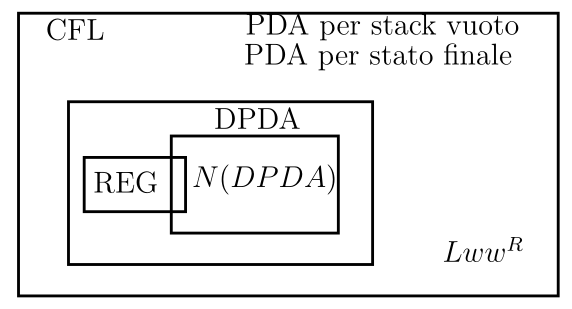
\includegraphics{2025-01-16_15-07.png}
		% \psscalebox{1.0 1.0} % Change this value to rescale the drawing.
		% {
		% 	\begin{pspicture}(0,-2.0)(7.6,2.0)
		% 		\psframe[linecolor=black, linewidth=0.04, dimen=outer](7.6,2.0)(0.0,-2.0)
		% 		\psframe[linecolor=black, linewidth=0.04, dimen=outer](5.0,0.76)(0.7,-1.56)
		% 		\psframe[linecolor=black, linewidth=0.04, dimen=outer](2.38,-0.02)(0.92,-0.82)
		% 		\rput[bl](0.4,1.6){CFL}
		% 		\rput[bl](1.066,-0.54){REG}
		% 		\rput[bl](2.76,0.36){DPDA}
		% 		\rput[bl](3.18,1.18){PDA per stato finale}
		% 		\rput[bl](3.2,1.6){PDA per stack vuoto}
		% 		\rput[bl](5.96,-1.5){$Lww^R$}
		% 		\psframe[linecolor=black, linewidth=0.04, dimen=outer](4.52,0.28)(2.14,-1.12)
		% 		\rput[bl](2.45,-0.56){$N(DPDA)$}
		% 	\end{pspicture}
		% }

	\end{center}
	SI ha che $L_{wcw^R}$ gode della proprietà di prefisso:
	$$y=wcw^R\in L\,\, Se\,\,x\neq y,\mbox{ prefisso di } y,x\not\in L$$
	tornando alle grammatiche si hanno ora due teoremi:
	\begin{theorem}
		se $L=N(P)$ per un DPDA P, allora L ha una CFG non ambigua
	\end{theorem}
	\begin{theorem}
		se $L=L(P)$ per un DPDA P, allora L ha una CFG non ambigua
	\end{theorem}
	dimostriamo il secondo:
	\begin{proof}
		$L=L(P)$ per un DPDA P, costruiamo $L^{'}=L$, quindi $L^{'}$ ha la proprietà di prefisso. Esiste quindi un DPDA $P^{'}$ tale che $L^{'}N(P)$, esiste quindi per il teorema sopra una CFG $G^{'}$ tale che $L(G^{'})=L^{'}$ che non è ambigua.\\
		Costruiamo $G$ per $L$ con le stesse produzioni di $G^{'}$ più $\$\to\varepsilon$, applicata solo all'ultimo passo.
	\end{proof}
	Vogliamo scoprire se è vero il viceversa: per ogni L che ha una CFG non ambigua è vero che L è
	accettato da un DPDA? No, mostriamo infatti un controesempio:\\
$S\to 0S0|1S1|\varepsilon$ produce $L_{ww^R}$ che non è accettato da alcun PDA

	\begin{Exercise}
		costruire un PDA per $L=\{0^n  n| n\geq 1\}$:
		CONTROLLARE LINGUAGGIO
		\begin{center}
			\begin{tikzpicture}[shorten >=1pt,node distance=3cm,on grid,auto]
				\node[state, initial] (q_0) {$q_0$};
				\node[state] (q_1) [right=of q_0] {$q_1$};
				\node[state, accepting] (q_2) [right =of q_1] {$q_2$} ;
				\path[->]
				(q_0) edge [loop above] node [align=center] {$0,0/00$\\$0,z_0/0z_0$} ()
				edge node [align=center] {$1,0/\varepsilon$} (q_1)
				(q_1) edge node {$\varepsilon,z_0/\varepsilon$} (q_2)
				edge [loop above] node [align=center] {$1,0/\varepsilon$} ();
			\end{tikzpicture}
		\end{center}
		Osserviamo che questo è un DPDA e L è accettato sia per stato finale che per stack vuoto.
		Osserviamo anche che L ha la proprietà di prefisso:
		$$y=0^n1^n\in L,x\neq y$$
		e $x$ è prefissa di y e quindi x ha un numero di 0 diverso da quelli di 1 e quindi $x\not\in L$
	\end{Exercise}

	\begin{Exercise}
		costruire un PDA per $L=\{0^n  n|\,n\geq 0\}$:
		\begin{center}
			\begin{tikzpicture}[shorten >=1pt,node distance=3cm,on grid,auto]
				\node[state, initial] (q_0) {$q_0$};
				\node[state] (q_1) [right=of q_0] {$q_1$};
				\node[state, accepting] (q_2) [right =of q_1] {$q_2$} ;
				\path[->]
				(q_0) edge [loop above] node [align=center] {$0,0/00$\\$0,z_0/0z_0$} ()
				edge node [align=center] {$1,0/\varepsilon$} (q_1)
				edge [bend left = 25] node {$\varepsilon,z_0/\varepsilon$} (q_2)
				(q_1) edge node {$\varepsilon,z_0/\varepsilon$} (q_2)
				edge [loop below] node [align=center] {$1,0/\varepsilon$} ();
			\end{tikzpicture}
		\end{center}
		Ora la stringa vuota appartiene al linguaggio. Il linguaggio non ha la proprietà del prefisso. Si può dimostrare che non esiste un DPDA per L.
	\end{Exercise}
	\begin{Exercise}
		considero il linguaggio generato da $B\to (BB)|(B)|()$.\\
		Il linguaggio ha la proprietà di prefisso perché (BB). Se fosse B -> BB allora non lo avrebbe, perché potremmo costruire le stringhe () e ()().
		\\Abbiamo quindi il DPDA per stato finale:
		\begin{center}
			\begin{tikzpicture}[shorten >=1pt,node distance=3cm,on grid,auto]
				\node[state, initial] (q_0) {$q_0$};
				\node[state] (q_1) [right=of q_0] {$q_1$};
				\node[state, accepting] (q_2) [right =of q_1] {$q_2$} ;
				\path[->]
				(q_0) edge [loop above] node [align=center] {$(,z_0/(z_0$\\$(,(/(($} ()
				edge [bend left = 25] node [align=center] {$),(/\varepsilon$} (q_1)

				(q_1) edge node {$\varepsilon,z_0/\varepsilon$} (q_2)
				edge [bend left = 25] node {$(,(/(($} (q_0)
				edge [loop above] node [align=center] {$),(/\varepsilon$} ();
			\end{tikzpicture}
		\end{center}
		volendo accettare solo per stack vuoto:
		\begin{center}
			\begin{tikzpicture}[shorten >=1pt,node distance=3cm,on grid,auto]
				\node[state, initial] (q_0) {$q_0$};
				\node[state] (q_1) [right=of q_0] {$q_1$};
				\path[->]
				(q_0) edge [loop above] node [align=center] {$(,z_0/(z_0$\\$(,(/(($} ()
				edge [bend left = 25] node [align=center] {$),(/\varepsilon$} (q_1)

				(q_1) edge [bend left = 25] node {$(,(/(($} (q_0)
				edge [loop above] node [align=center] {$),(/\varepsilon$ \\ $\varepsilon,z_0/\varepsilon$} ();
			\end{tikzpicture}
		\end{center}
	\end{Exercise}
	\begin{Exercise}
		Si ha $B\to BB|(B)|()$. La stringa vuota non appartiene al linguaggio ma L non ha la proprietà del prefisso (come abbiamo
		mostrato nell'esercizio precedente). Possiamo quindi realizzare solo un DPDA per stato finale:
		\begin{center}
			\begin{tikzpicture}[shorten >=1pt,node distance=3cm,on grid,auto]
				\node[state, initial] (q_0) {$q_0$};
				\node[state] (q_1) [right=of q_0] {$q_1$};
				\node[state] (q_2) [right =of q_1] {$q_2$};
				\node[state,accepting] (q_3) [below right =of q_1] {$q_3$};
				\path[->]
				(q_0) edge node [align=center] {$(,z_0/(z_0$} (q_1)

				(q_1) edge [bend left = 25] node {$),(/\varepsilon$} (q_2)
				edge [loop above] node [align=center] {$(,(/(($} ()
				(q_2) edge [bend left = 25] node {$(,(/(($} (q_1)
				edge [loop above] node [align=center] {$),(/\varepsilon$} ()
				edge node {$\varepsilon,z_0/z_0$} (q_3)
				(q_3) edge node {$(,z_0/(z_0$} (q_1)  ;
			\end{tikzpicture}
		\end{center}
	\end{Exercise}
	\begin{Exercise}
		Si ha $B\to BB|(B)|\varepsilon$ ho un DPDA per stato finale perché L non ha la proprietà del prefisso:
		\begin{center}
			\begin{tikzpicture}[shorten >=1pt,node distance=3cm,on grid,auto]
				\node[state, initial,accepting] (q_0) {$q_0$};
				\node[state] (q_1) [right=of q_0] {$q_1$};
				\node[state] (q_2) [right =of q_1] {$q_2$};

				\path[->]
				(q_0) edge node [align=center] {$(,z_0/(z_0$} (q_1)

				(q_1) edge [bend left = 25] node {$),(/\varepsilon$} (q_2)
				edge [loop above] node [align=center] {$(,(/(($} ()
				(q_2) edge [bend left = 25] node {$(,(/(($} (q_1)
				edge [loop above] node [align=center] {$),(/\varepsilon$} ()
				edge [bend left = 65] node {$\varepsilon,z_0/z_0$} (q_0);
			\end{tikzpicture}
		\end{center}
	\end{Exercise}
	\begin{Exercise}
		sia $L=\{q\in\{a,b\}^*| numero\,\,uguale\,\,di\,\,a\,\,e\,\,b\}$ DPDA per stato finale (L non ha la proprietà di prefisso):
		\begin{center}
			\begin{tikzpicture}[shorten >=1pt,node distance=3cm,on grid,auto]
				\node[state, initial,accepting] (q_0) {$q_0$};
				\node[state] (q_1) [right=of q_0] {$q_1$};
				\path[->]
				(q_0) edge [bend left=25] node [align=center] {$b,z_0/bz_0$\\$a,z_0/az_0$} (q_1)

				(q_1) edge [bend left = 25] node {$\varepsilon,z_0/z_0$} (q_0)
				edge [loop above] node [align=center] {$a,a/aa$\\$b,b/bb$\\$a,b/\varepsilon$ \\$b,a/\varepsilon$} ()
				;
			\end{tikzpicture}
		\end{center}
	\end{Exercise}
	\newpage
	\begin{Exercise}
		sia dato il CFL $L=\{a^ncb^n|n\geq 0\}$\\
		è generato da :
		$$G=(\{S\},\{a,b,c\},P,S)$$
		$$S\to aSb|c$$
		si ha il seguente automa non deterministico:
		\begin{center}
			\begin{tikzpicture}[shorten >=1pt,node distance=3cm,on grid,auto]
				\node[state, initial,accepting] (q_0) {$q_0$};
				\path[->]
				(q_0) edge [loop above] node [align=center] {$\varepsilon,S/aSb$\\$\varepsilon,S/c$\\$a,a/\varepsilon$\\$b,b/\varepsilon$\\$c,c/\varepsilon$} ();
			\end{tikzpicture}
		\end{center}
		con:
		$$\delta(q,\varepsilon,S)=\{(q,aSb),(q,c)\}$$
		$$\delta(q,a,a)=\{(q,\varepsilon)\}$$
		$$\delta(q,b,b)=\{(q,\varepsilon)\}$$
		$$\delta(q,c,c)=\{(q,\varepsilon)\}$$
		mostro la derivazione per n=3, aaacbbb e il comportamento dell'automa:
		$$(q,aaacbbb,S)\vdash(q,aaacbbb,aSb)\vdash(q,aacbb,Sb)\vdash(q,aacbb,aSb)$$
		$$\vdash(q,acbbb,Sbb)\vdash(q,acbbb,aSbbb)\vdash(q,cbbb,Sbbbb)\vdash(q,cbbb,cbbb)$$
		$$\vdash(q,bbb,bbb)\vdash(q,bb,bb)\vdash(q,b,b)\vdash(q,\varepsilon,\varepsilon)\to \,\, accetta$$
		si ha che vale la proprietà del prefisso e si ha il seguente DPDA:
		\begin{center}
			\begin{tikzpicture}[shorten >=1pt,node distance=3cm,on grid,auto]
				\node[state, initial,accepting] (q_0) {$q_0$};
				\node[state] (q_1) [right=of q_0] {$q_1$};
				\node[state] (q_2) [right =of q_1] {$q_2$};
				\path[->]
				(q_0) edge node [align=center] {$c,z_0/cz_0$\\$c,a/a$} (q_1)
				edge [loop above] node [align=center] {$a,z_0/az_0$\\$a,a/aa$} ()
				(q_1) edge  node {$\varepsilon,z_0/z_0$} (q_2)
				edge [loop above] node [align=center] {$b,a/\varepsilon$} ();
			\end{tikzpicture}
		\end{center}
	\end{Exercise}
	\begin{Exercise}
		realizzare il pda per $L=\{a^nb^mcd^mef^n|n,m\geq 0\}$;
		si ha quindi:
		$$a^ncef^n\,\,n>0$$
		$$b^mcd^me\,\,m>0$$
		$$a^nb^mcd^mef^n\,\,n,m> 0$$
		$$ce\,\,n=0=m$$
		\begin{center}
			\begin{tikzpicture}[shorten >=1pt,node distance=3cm,on grid,auto]
				\node[state, initial] (q_0) {$q_0$};
				\node[state] (q_1) [above right=of q_0] {$\mbox{ }$};
				\node[state] (q_2) [right =of q_0] {$\mbox{ }$};
				\node[state] (q_3) [below right =of q_0] {$\mbox{ }$};
				\node[state] (q_4) [ right =of q_1] {$\mbox{ }$};
				\node[state] (q_5) [above =of q_1] {$\mbox{ }$};
				\node[state] (q_6) [right =of q_2] {$\mbox{ }$};
				\node[state,accepting] (q_7) [right =of q_6] {$\mbox{ }$};
				\node[state] (q_8) [right =of q_5] {$\mbox{ }$};
				\node[state] (q_9) [right =of q_8] {$\mbox{ }$};
				\node[state] (q_a) [right =of q_4] {$\mbox{ }$};

				\path[->]
				(q_0) edge node [align=center] {$a,z_0/az_0$} (q_1)
				(q_0) edge node [align=center] {$b,z_0/bz_0$} (q_2)
				(q_0) edge node [left] {$c,z_0/cz_0$} (q_3)
				(q_2) edge node [align=center] {$c,b/b$} (q_6)
				edge [loop below] node [align=center] {$b,b/bb$} ()
				(q_6) edge node [align=center] {$\varepsilon,z_0/z_0$} (q_7)
				edge [loop below] node [align=center] {$d,b/\varepsilon$} ()

				(q_3) edge [bend right =65] node [align=center] {$\varepsilon,z_0/z_0$} (q_7)
				(q_1) edge node [align=center] {$b,a/ba$} (q_5)
				edge node [align=center] {$c,a/ca$} (q_4)
				edge [loop left] node [align=center] {$a,a/aa$} ()
				(q_5) edge node [align=center] {$c,b/cb$} (q_8)
				edge [loop above] node [align=center] {$b,b/bb$} ()
				(q_8) edge node [align=center] {$e,a/a$} (q_9)
				edge [loop above] node [align=center] {$d,b/\varepsilon$} ()
				(q_9) edge [bend left =95] node [align=center] {$\varepsilon,z_0/z_0$} (q_7)
				edge [loop above] node [align=center] {$f,a/\varepsilon$} ()
				(q_4) edge node [align=center] {$e,a/a$} (q_a)
				(q_a) edge node [align=center] {$\varepsilon,z_0/z_0$} (q_7)
				edge [loop right] node [align=center] {$f,a/\varepsilon$} ()
				;


			\end{tikzpicture}
		\end{center}
	\end{Exercise}

	\newpage
\section{Soluzioni degli esercizi}
\label{sec:soluzioni-cfg}
\shipoutAnswer

%%% Local Variables:
%%% mode: LaTeX
%%% TeX-master: ../libro-linguaggi
%%% End:



\parte{Computabilità}\label{part:turing}
%\setchapterpreamble[u]{\margintoc}
	\chapter{Macchine di Turing}
	Nascono in risposta al problema di Hilbert, che si chiedeva se esiste un algoritmo per dimostrare teoremi. Non ci sono comunque funzioni non calcolabili con le macchine di Turing:
	$$f:\mathbb{N}\to\{0,1\}\,\,s^{|\mathbb{N}}|>\mathbb{N}$$
	Siamo interessati a studiare la calcolabilità (computabilità).
	Esiste un programma che calcola una certa funzione? Se non esiste, $f$ è indecidibile. Se sì, in quanto tempo è calcolabile (complessità computazionale), quante mosse e quante celle del nastro sono necessarie?\\
	vediamo due esempi:
	\begin{example}
		data una CFG $G=(V,T,P,S)$ stabilire se è ambigua. Questo problema è indecidibile, cioè non esiste nessun algoritmo che dia una risposta.
	\end{example}
	\begin{example}
		Problema "ciao mondo": dato un sorgente di un programma in C/Java/..., i primi undici caratteri
		stampati dal programma sono "ciao, mondo"?
		Consideriamo il seguente algoritmo, che prende in input un numero intero N e stampa "ciao mondo" sse $\exists x,y,z\in \mathbb{N}$ tali che $x^n+y^n=z^n$
	\end{example}
	quest'ultimo problema è indecidibile:
	\begin{proof}
		procediamo per assurdo.\\Supponiamo che esista un algoritmo che risolva il problema.
		Assumiamo che P sia corretto (e quindi compilabile) e che stampi solo stringhe sulla console:
		\begin{center}
		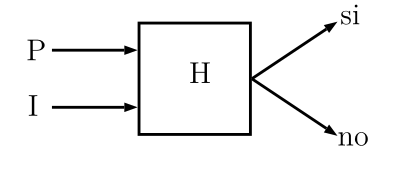
\includegraphics{2025-01-16_15-09.png}
			%\psscalebox{1.0 1.0} % Change this value to rescale the drawing.
			%{
			%	\begin{pspicture}(0,-0.965)(4.71,0.965)
			%		\psframe[linecolor=black, linewidth=0.04, dimen=outer](3.16,0.775)(1.56,-0.825)
			%		\psline[linecolor=black, linewidth=0.04, arrowsize=0.05291667cm 2.0,arrowlength=1.4,arrowinset=0.0]{->}(0.36,-0.425)(1.56,-0.425)
			%		\psline[linecolor=black, linewidth=0.04, arrowsize=0.05291667cm 2.0,arrowlength=1.4,arrowinset=0.0]{->}(0.36,0.375)(1.56,0.375)
			%		\psline[linecolor=black, linewidth=0.04, arrowsize=0.05291667cm 2.0,arrowlength=1.4,arrowinset=0.0]{->}(3.16,-0.025)(4.36,0.775)
			%		\psline[linecolor=black, linewidth=0.04, arrowsize=0.05291667cm 2.0,arrowlength=1.4,arrowinset=0.0]{->}(3.16,-0.025)(4.36,-0.825)
			%		\rput[bl](0.0,0.235){P}
			%		\rput[bl](0.02,-0.545){I}
			%		\rput[bl](2.28,-0.085){H}
			%		\rput[bl](4.4,0.735){si}
			%		\rput[bl](4.36,-0.965){no}
			%	\end{pspicture}
			%}
		\end{center}
		quindi:
		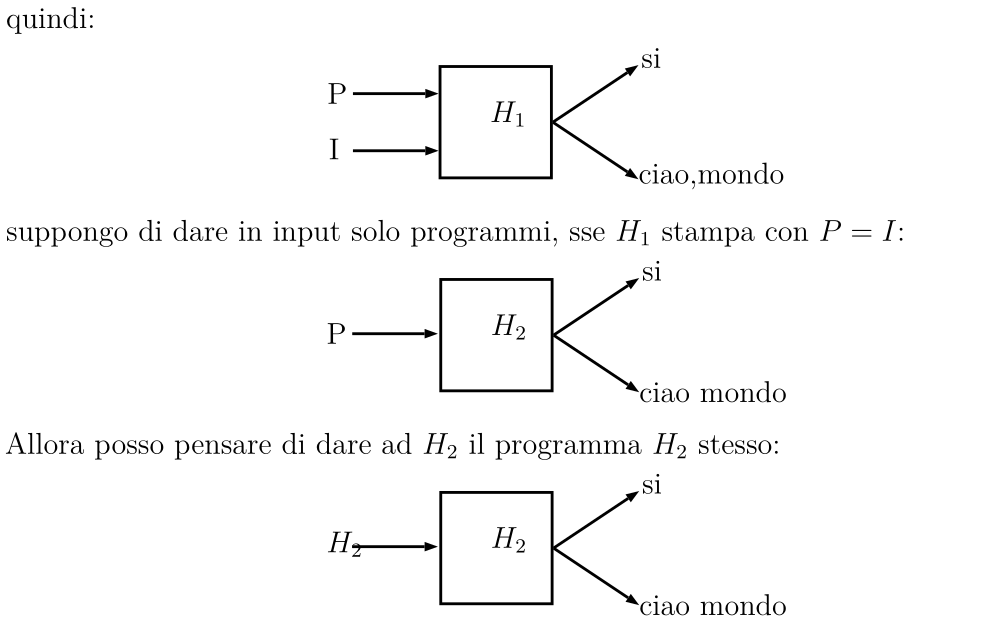
\includegraphics{2025-01-16_15-10.png}
		suppongo di dare in input solo programmi, sse $H_1$ stampa con $P=I$:
		Allora posso pensare di dare ad $H_2$ il programma $H_2$ stesso:
		Ma questo è assurdo: perché $H_2$ dice si quando in realtà stampa ciao mondo e viceversa, quindi
		non funziona. Ma allora in conclusione H non può esistere (perché i passaggi da H a $H_1$ e da $H_1$ a
		$H_2$ sono leciti) e quindi il problema non è decidibile.
	\end{proof}
	\section{Riduzioni}
	Supponiamo $P_2$ indicibile. Considerato un nuovo problema $P_2$, vorrei stabilire se anch'esso è
	indecidibile. Vorremmo quindi fare una "riduzione" da $P_1$ a $P_2$:
		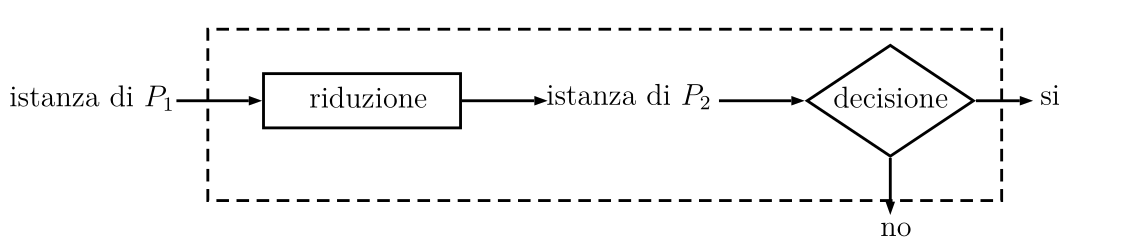
\includegraphics{2025-01-16_15-12.png}

	Supponiamo per assurdo che $P_2$ sia decidibile. Allora esiste l'algoritmo di decisione. Esistendo il
	processo di riduzione, allora l'intero rettangolo tratteggiato sarebbe un algoritmo di decisione per
$P_1$, assurdo perché $P_1$ è indecidibile per ipotesi.
	\begin{example}
		$P_2$ (Problema della chiamata): dato un programma $Q$, esso chiama il metodo $m()$?
		\\Dobbiamo quindi trovare un algoritmo di riduzione. Procediamo:
		\begin{itemize}
			\item rinominiamo tutte le istanze di $m$ in qualcosa d'altro
			\item aggiungiamo un metodo m che non verrà quindi mai chiamato
			\item modifichiamo questo programma in modo che salvi in un array i primi 11 caratteri che stampa a video
			\item modifichiamo questo programma in modo che se sfora gli 11 caratteri e controlla tali caratteri. Se sono esattamente "ciao mondo", chiama m
		\end{itemize}
		quindi anche questo problema è indecidibile
	\end{example}
	È importante che la riduzione sia fatta nel verso corretto. Se facessimo la riduzione da $P_2$ a $P_1$,
	staremmo mostrando che se $P_1$ è decidibile allora $P_2$ è decidibile. Ma sappiamo che $P_1$ è
	indecidibile, quindi non staremmo dimostrando niente.
	Nel caso contrario stiamo invece dicendo che se $P_2$ è decidibile allora $P_1$ è decidibile. Ma essendo
$P_1$ indecidibile, allora l'antecedente è falsa e quindi $P_2$ non può essere decidibile, quindi è
	indecidibile.\\
	Diamo ora la definizione formale della Macchina di Turing:
	\begin{definition}
		Si definisce MdT:
		$$M=(Q,\Sigma,\Gamma,\delta,q_0,B,F)$$
		con:
		\begin{itemize}
			\item $Q$ insieme finito non vuoto di stati
			\item $\Sigma$ insieme finito non vuoto di simboli di input
			\item $\Gamma$ insieme finito non vuoto di simboli sul nastro
			\item $\delta:Q\times\Gamma\to Q\times\Gamma\times\{L,R\}$
			\item $q_0\in Q$ stato iniziale
			\item $B\in\Gamma\backslash\Sigma$ simboli di blank
			\item $F\subseteq Q$ insieme di stati finali
		\end{itemize}
		inoltre si ha che:
		$$\Sigma\subseteq \Gamma\,\,\,e\,\,\,\Gamma\cap\Sigma\neq\emptyset$$
		quindi si ha per esempio questa rappresentazione, per l'input $x_1,...,x_n\in\Sigma^*$:
		\begin{center}
		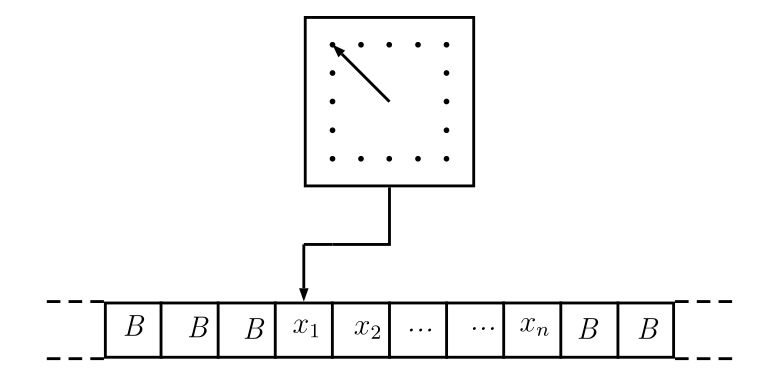
\includegraphics{2025-01-16_15-13.png}

			%\psscalebox{1.0 1.0} % Change this value to rescale the drawing.
			%{
			%	\begin{pspicture}(0,-2.41)(9.540835,2.41)
			%		\psframe[linecolor=black, linewidth=0.04, dimen=outer](6.0,2.41)(3.6,0.01)
			%		\psframe[linecolor=black, linewidth=0.04, dimen=outer](8.8,-1.59)(0.8,-2.39)
			%		\psline[linecolor=black, linewidth=0.04](4.8,0.01)(4.8,-0.79)(4.0,-0.79)
			%		\psline[linecolor=black, linewidth=0.04](1.6,-1.59)(1.6,-2.39)
			%		\psline[linecolor=black, linewidth=0.04](2.4,-1.59)(2.4,-2.39)
			%		\psline[linecolor=black, linewidth=0.04](3.2,-1.59)(3.2,-2.39)
			%		\psline[linecolor=black, linewidth=0.04](4.0,-1.59)(4.0,-2.39)
			%		\psline[linecolor=black, linewidth=0.04](4.8,-1.59)(4.8,-2.39)
			%		\psline[linecolor=black, linewidth=0.04](5.6,-1.59)(5.6,-2.39)
			%		\psline[linecolor=black, linewidth=0.04](6.4,-1.59)(6.4,-2.39)
			%		\psline[linecolor=black, linewidth=0.04](7.2,-1.59)(7.2,-2.39)
			%		\psline[linecolor=black, linewidth=0.04](8.0,-1.59)(8.0,-2.39)
			%		\psline[linecolor=black, linewidth=0.04, linestyle=dashed, dash=0.17638889cm 0.10583334cm](0.0,-1.59)(0.8,-1.59)
			%		\psline[linecolor=black, linewidth=0.04, linestyle=dashed, dash=0.17638889cm 0.10583334cm](0.0,-2.39)(0.8,-2.39)
			%		\psline[linecolor=black, linewidth=0.04, linestyle=dashed, dash=0.17638889cm 0.10583334cm](8.8,-1.59)(9.6,-1.59)
			%		\psline[linecolor=black, linewidth=0.04, linestyle=dashed, dash=0.17638889cm 0.10583334cm](8.8,-2.39)(9.6,-2.39)
			%		\psdots[linecolor=black, dotsize=0.08](4.0,2.01)
			%		\psdots[linecolor=black, dotsize=0.08](5.6,2.01)
			%		\psdots[linecolor=black, dotsize=0.08](5.6,1.21)
			%		\psdots[linecolor=black, dotsize=0.08](5.2,0.41)
			%		\psdots[linecolor=black, dotsize=0.08](4.4,0.41)
			%		\psdots[linecolor=black, dotsize=0.08](4.8,2.01)
			%		\psdots[linecolor=black, dotsize=0.08](4.0,1.21)
			%		\psdots[linecolor=black, dotsize=0.08](4.0,0.41)
			%		\psdots[linecolor=black, dotsize=0.08](5.6,0.41)
			%		\psdots[linecolor=black, dotsize=0.08](4.8,0.41)
			%		\psdots[linecolor=black, dotsize=0.08](4.4,2.01)
			%		\psdots[linecolor=black, dotsize=0.08](5.2,2.01)
			%		\psdots[linecolor=black, dotsize=0.08](5.6,1.61)
			%		\psdots[linecolor=black, dotsize=0.08](5.6,0.81)
			%		\psdots[linecolor=black, dotsize=0.08](4.0,1.61)
			%		\psdots[linecolor=black, dotsize=0.08](4.0,0.81)
			%		\psline[linecolor=black, linewidth=0.04, arrowsize=0.05291667cm 2.0,arrowlength=1.4,arrowinset=0.0]{->}(3.6,-0.79)(3.6,-1.59)
			%		\psline[linecolor=black, linewidth=0.04, arrowsize=0.05291667cm 2.0,arrowlength=1.4,arrowinset=0.0]{->}(4.8,1.21)(4.0,2.01)
			%		\psline[linecolor=black, linewidth=0.04](4.0,-0.79)(3.6,-0.79)
			%		\rput[bl](3.44,-2.09){$x_1$}
			%		\rput[bl](6.62,-2.07){$x_n$}
			%		\rput[bl](4.3,-2.11){$x_2$}
			%		\rput[bl](5.04,-2.01){...}
			%		\rput[bl](5.92,-1.99){...}
			%		\rput[bl](7.42,-2.11){B}
			%		\rput[bl](8.26,-2.11){B}
			%		\rput[bl](2.74,-2.11){B}
			%		\rput[bl](1.96,-2.09){B}
			%		\rput[bl](1.06,-2.07){B}
			%	\end{pspicture}
			%}

		\end{center}
	\end{definition}
	\newpage
	Questa era una definizione deterministica, passiamo ora ad una definizione \textit{istantanea}:
	\begin{definition}
		suppongo di avere lo stato $q$, il nastro $x_1,...,x_n$ con la testina $x_i$. SI ha:
		$$ID:\,\,x_1x_2,...qx_ix_{i+1}...x_n$$
		e suppongo $Q\cap\Gamma=\emptyset$ senza perdere generalità e uso la simbologia dei $\vdash$ introdotta coi PDA. \\
		Se $\delta(q,x_i)=(p,y,L)$ allora $\vdash\,\, x_1x_2...x_{i-2}px_{i-1}yx_{i+1}...x_n$.\\
		Si hanno dei casi particolari:
		\begin{itemize}
			\item se $i=1$ si ha $qx_1x_2...x_n\vdash pByx_2...x_n$
			\item se $i=n\,\,y=B$ si ha $qx_1x_2...qx_n\vdash x_1x_2...x_{n-2}px_{n-1}$
		\end{itemize}
		a destra abbiamo invece:
		Se $\delta(q,x_i)=(p,y,R)$ allora $\vdash\,\, x_1x_2...x_{i-1}Ypx_{i+1}...x_n$.\\
		Si hanno dei casi particolari:
		\begin{itemize}
			\item se $i=1$ si ha $q_1x_2...x_{n-1}\vdash ypB$
			\item se $i=n\,\,y=B$ si ha $qx_1x_2...qx_n\vdash px_2...x_n$
		\end{itemize}
	\end{definition}
	\begin{example}
		sia $L=\{0^n1^n|\,n\geq 1\}$ un CFL. vediamo una tabella per capire l'azione della macchina:
		\begin{center}
			\begin{tabular}{c|c|c|c|c|c|}
				      & 0           & 1           & x           & y           & B           \\
				\hline
				$q_0$ & $(q_1,x,R)$ & --          & --          & $(q_3,y,R)$ & --          \\
				$q_1$ & $(q_1,0,R)$ & $(q_2,y,L)$ & --          & $(q_1,y,R)$ & --          \\
				$q_2$ & $(q_2,0,L)$ & --          & $(q_0,x,R)$ & $(q_2,y,L)$ & --          \\
				$q_3$ & --          & --          & --          & $(q_2,y,L)$ & $(q_4,B,R)$ \\
				$q_4$ & --          & --          & --          & --          & --
			\end{tabular}
		\end{center}
		ovvero, per esempio:
		$$000111$$
		$$x00111$$
		$$x00y11$$
		$$xx0yy1$$
		$$xxxyyy$$
		\newpage
		ma la tabella non è comodissima, usiamo quindi i diagrammi di transizione:
		\begin{center}
			\begin{tikzpicture}[shorten >=1pt,node distance=3cm,on grid,auto]
				\node[state, initial,accepting] (q_0) {$q_0$};
				\node[state] (q_1) [right=of q_0] {$q_1$};
				\node[state] (q_2) [right =of q_1] {$q_2$};
				\node[state] (q_3) [below =of q_0] {$q_3$};
				\node[state] (q_4) [right =of q_3] {$q_4$};

				\path[->]
				(q_0) edge node [align=center] {$0/x\rightarrow$} (q_1)
				edge node [align=center] {$y/y\rightarrow$} (q_3)
				(q_1) edge node {$1/y\leftarrow$} (q_2)
				edge [loop above] node [align=center] {$y/y\rightarrow$\\$0/0\rightarrow$} ()
				(q_2) edge [bend left =40] node {$x/x\rightarrow$} (q_0)
				edge [loop above] node [align=center] {$y/y\leftarrow$\\$0/0\leftarrow$} ()
				(q_3) edge  node {$B/B\rightarrow$} (q_4)
				edge [loop below] node [align=center] {$y/y\rightarrow$} ()
				;
			\end{tikzpicture}
		\end{center}
		e per l'input 0010 si hanno i seguenti passi:
		$$q_0010\vdash xq_1010\vdash x0q_110\vdash xq_20y0\vdash  q_2x0y0$$
		$$\vdash xxq_2y0\vdash xxyq_10\vdash xxy0q_1B$$
	\end{example}
	definiamo quini il linguaggio accettato da una macchina di Turing:
	$$M=(Q,\Sigma,\Gamma,\delta,q_0,B,F)$$
	$$L(M)=\{w\in\Sigma^*|q_0w\stackrel{*}{\vdash}\alpha p\beta\,\,p\in F\,\,\alpha,\beta\in\Gamma^*\}$$
	La classe dei linguaggi accettati dalle MdT sono i ricorsivamente enumerabili (RE).
	Le MdT possono anche calcolare le funzioni:
	\begin{example}
		$$f(n,m)=m-n=max(m-n,0)=\begin{cases}
				m-n\,\,m\geq n \\
				0\,\,\,\,\,m<n
			\end{cases}$$
		quindi se l'input fosse $0^m10^n$ si avrebbe in output $0^{m-n}$
	\end{example}
	si ha che se la MdT accetta, allora si ferma e che se la MdT non accetta, allora non si può dire se si ferma oppure no. Se non si ferma: linguaggi ricorsivamente enumerabili. Se si ferma sempre, otteniamo una sottoclasse che sono i linguaggi ricorsivi. Inoltre il problema dell'arresto, \textbf{halting problem}, è indecidibile e quindi i linguaggi ricorsivamente enumerabili sono quindi semidecibili.\\
	Si possono avere delle estensioni della macchina di Turing:
	\begin{itemize}
		\item macchina non deterministica; anziché una sequenza di ID avremmo un albero. Non si aggiunge comunque potenza di calcolo, perché posso simulare una nondet con una det che esplora questo albero
		\item MdT multinastro
		      Hanno un numero finito di nastri. In una mossa guarda lo stato del controllo e il simbolo sotto ciascuna delle testine, si muove in un nuovo stato, scrive un nuovo simbolo per ogni nastro e si muove indipendentemente su ogni nastro:
		      \begin{center}
		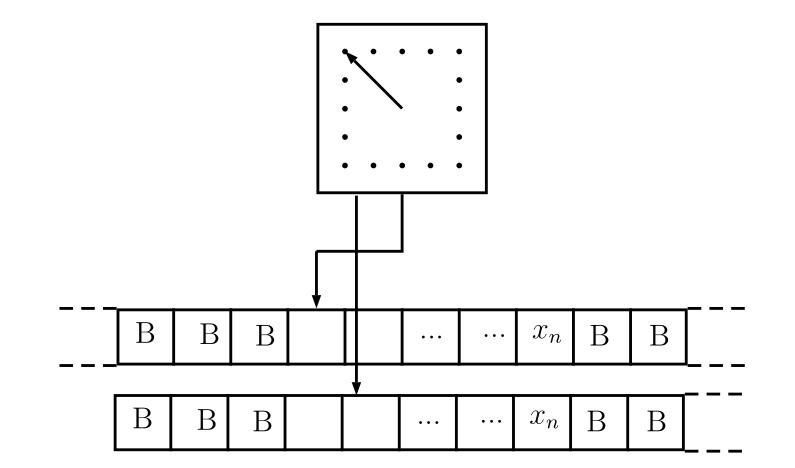
\includegraphics{2025-01-16_15-15.png}


			    %  \psscalebox{1.0 1.0} % Change this value to rescale the drawing.
			    %  {
				%      \begin{pspicture}(0,-3.01)(9.540835,3.01)
				%	      \psframe[linecolor=black, linewidth=0.04, dimen=outer](6.0,3.01)(3.6,0.61)
				%	      \psframe[linecolor=black, linewidth=0.04, dimen=outer](8.8,-0.99)(0.8,-1.79)
				%	      \psline[linecolor=black, linewidth=0.04](4.8,0.61)(4.8,-0.19)(4.0,-0.19)
				%	      \psline[linecolor=black, linewidth=0.04](1.6,-0.99)(1.6,-1.79)
				%	      \psline[linecolor=black, linewidth=0.04](2.4,-0.99)(2.4,-1.79)
				%	      \psline[linecolor=black, linewidth=0.04](3.2,-0.99)(3.2,-1.79)
				%	      \psline[linecolor=black, linewidth=0.04](4.0,-0.99)(4.0,-1.79)
				%	      \psline[linecolor=black, linewidth=0.04](4.8,-0.99)(4.8,-1.79)
				%	      \psline[linecolor=black, linewidth=0.04](5.6,-0.99)(5.6,-1.79)
				%	      \psline[linecolor=black, linewidth=0.04](6.4,-0.99)(6.4,-1.79)
				%	      \psline[linecolor=black, linewidth=0.04](7.2,-0.99)(7.2,-1.79)
				%	      \psline[linecolor=black, linewidth=0.04](8.0,-0.99)(8.0,-1.79)
				%%%%%%%%%%	      \psline[linecolor=black, linewidth=0.04, linestyle=dashed, dash=0.17638889cm 0.10583334cm](0.0,-0.99)(0.8,-0.99)
				%	      \psline[linecolor=black, linewidth=0.04, linestyle=dashed, dash=0.17638889cm 0.10583334cm](0.0,-1.79)(0.8,-1.79)
				%	      \psline[linecolor=black, linewidth=0.04, linestyle=dashed, dash=0.17638889cm 0.10583334cm](8.8,-0.99)(9.6,-0.99)
				%	      \psline[linecolor=black, linewidth=0.04, linestyle=dashed, dash=0.17638889cm 0.10583334cm](8.8,-1.79)(9.6,-1.79)
				%	      \psdots[linecolor=black, dotsize=0.08](4.0,2.61)
				%	      \psdots[linecolor=black, dotsize=0.08](5.6,2.61)
				%	      \psdots[linecolor=black, dotsize=0.08](5.6,1.81)
				%	      \psdots[linecolor=black, dotsize=0.08](5.2,1.01)
				%	      \psdots[linecolor=black, dotsize=0.08](4.4,1.01)
				%	      \psdots[linecolor=black, dotsize=0.08](4.8,2.61)
				%	      \psdots[linecolor=black, dotsize=0.08](4.0,1.81)
				%	      \psdots[linecolor=black, dotsize=0.08](4.0,1.01)
				%	      \psdots[linecolor=black, dotsize=0.08](5.6,1.01)
				%	      \psdots[linecolor=black, dotsize=0.08](4.8,1.01)
				%	      \psdots[linecolor=black, dotsize=0.08](4.4,2.61)
				%	      \psdots[linecolor=black, dotsize=0.08](5.2,2.61)
				%	      \psdots[linecolor=black, dotsize=0.08](5.6,2.21)
				%	      \psdots[linecolor=black, dotsize=0.08](5.6,1.41)
				%	      \psdots[linecolor=black, dotsize=0.08](4.0,2.21)
				%	      \psdots[linecolor=black, dotsize=0.08](4.0,1.41)
				%	      \psline[linecolor=black, linewidth=0.04, arrowsize=0.05291667cm 2.0,arrowlength=1.4,arrowinset=0.0]{->}(3.6,-0.19)(3.6,-0.99)
				%	      \psline[linecolor=black, linewidth=0.04, arrowsize=0.05291667cm 2.0,arrowlength=1.4,arrowinset=0.0]{->}(4.8,1.81)(4.0,2.61)
				%	      \psline[linecolor=black, linewidth=0.04](4.0,-0.19)(3.6,-0.19)
				%	      \rput[bl](6.62,-1.47){$x_n$}
				%	      \rput[bl](5.04,-1.41){...}
				%	      \rput[bl](5.92,-1.39){...}
				%	      \rput[bl](7.42,-1.51){B}
				%	      \rput[bl](8.26,-1.51){B}
				%	      \rput[bl](2.74,-1.51){B}
				%	      \rput[bl](1.96,-1.49){B}
				%	      \rput[bl](1.06,-1.47){B}
				%	      \psframe[linecolor=black, linewidth=0.04, dimen=outer](8.76,-2.19)(0.76,-2.99)
				%	      \psline[linecolor=black, linewidth=0.04](1.56,-2.19)(1.56,-2.99)
				%	      \psline[linecolor=black, linewidth=0.04](2.36,-2.19)(2.36,-2.99)
				%	      \psline[linecolor=black, linewidth=0.04](3.16,-2.19)(3.16,-2.99)
				%	      \psline[linecolor=black, linewidth=0.04](3.96,-2.19)(3.96,-2.99)
				%	      \psline[linecolor=black, linewidth=0.04](4.76,-2.19)(4.76,-2.99)
				%	      \psline[linecolor=black, linewidth=0.04](5.56,-2.19)(5.56,-2.99)
				%	      \psline[linecolor=black, linewidth=0.04](6.36,-2.19)(6.36,-2.99)
				%	      \psline[linecolor=black, linewidth=0.04](7.16,-2.19)(7.16,-2.99)
				%	      \psline[linecolor=black, linewidth=0.04](7.96,-2.19)(7.96,-2.99)
				%	      \psline[linecolor=black, linewidth=0.04, linestyle=dashed, dash=0.17638889cm 0.10583334cm](8.76,-2.19)(9.56,-2.19)
				%	      \psline[linecolor=black, linewidth=0.04, linestyle=dashed, dash=0.17638889cm 0.10583334cm](8.76,-2.99)(9.56,-2.99)
				%	      \psline[linecolor=black, linewidth=0.04, arrowsize=0.05291667cm 2.0,arrowlength=1.4,arrowinset=0.0]{->}(4.16,0.59)(4.16,-2.21)
				%	      \rput[bl](6.58,-2.67){$x_n$}
				%	      \rput[bl](5.0,-2.61){...}
				%	      \rput[bl](5.88,-2.59){...}
				%	      \rput[bl](7.38,-2.71){B}
				%	      \rput[bl](8.22,-2.71){B}
				%	      \rput[bl](2.7,-2.71){B}
				%	      \rput[bl](1.92,-2.69){B}
				%	      \rput[bl](1.02,-2.67){B}
				%      \end{pspicture}
			    %  }

		      \end{center}
	\end{itemize}
	si ha il seguente teorema:
	\begin{theorem}
		ogni linguaggio accettato da una MdT multinastro è Ricorsivamente Enumerabile
	\end{theorem}
	Ora possiamo definire in maniera più precisa cosa si intendeva per simulazione di una macchina
	nondet: uso due nastri, il primo con l'input e il secondo gestito come una coda di ID da elaborare
	\begin{theorem}
		Se Mn è una NTM (Nondeterministic Turing Machine) allora esiste una DTM
		(Deterministic Turing Machine) tale che il linguaggio accettato dalla NTM è uguale a quello accettato
		dalla DTM
	\end{theorem}
	\section{Restrizioni delle macchine di Turing}
	Consideriamo una MdT con nastro semiinfinito (ovvero è infinito solo da un lato):
	\begin{center}
			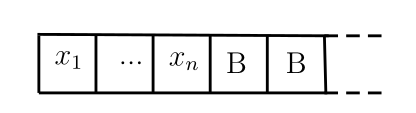
\includegraphics{2025-01-16_15-16.png}

		% \psscalebox{1.0 1.0} % Change this value to rescale the drawing.
		% {
		% 	\begin{pspicture}(0,-0.43)(4.7609334,0.43)
		% 		\psline[linecolor=black, linewidth=0.04](0.020098267,0.39)(0.020098267,-0.41)
		% 		\psline[linecolor=black, linewidth=0.04](0.8200983,0.39)(0.8200983,-0.41)
		% 		\psline[linecolor=black, linewidth=0.04](1.6200982,0.39)(1.6200982,-0.41)
		% 		\psline[linecolor=black, linewidth=0.04](2.4200983,0.39)(2.4200983,-0.41)
		% 		\psline[linecolor=black, linewidth=0.04](3.2200983,0.39)(3.2200983,-0.41)
		% 		\psline[linecolor=black, linewidth=0.04, linestyle=dashed, dash=0.17638889cm 0.10583334cm](4.020098,0.39)(4.8200984,0.39)
		% 		\psline[linecolor=black, linewidth=0.04, linestyle=dashed, dash=0.17638889cm 0.10583334cm](4.020098,-0.41)(4.8200984,-0.41)
		% 		\rput[bl](1.8400983,-0.09){$x_n$}
		% 		\rput[bl](0.24009827,-0.07){$x_1$}
		% 		\rput[bl](1.1400982,-0.01){...}
		% 		\rput[bl](2.6400983,-0.13){B}
		% 		\rput[bl](3.4800982,-0.13){B}
		% 		\psline[linecolor=black, linewidth=0.04](0.0,0.41)(4.080098,0.39)
		% 		\psline[linecolor=black, linewidth=0.04](0.020098267,-0.41)(4.040098,-0.41)(4.020098,0.39)
		% 	\end{pspicture}
		% }
	\end{center}
	si ha il seguente teorema:
	\begin{theorem}
		Ogni linguaggio accettato da una DTM M2 è anche accettato da una DTM M1 tale che:
		\begin{itemize}
			\item La testina di M1 non va mai a sinistra della posizione iniziale
			\item M1 non scrive mai un Blank:
			      $$B^{'}\not\in\Gamma \mbox{  e scrive }B^{'} \mbox{ al posto di } B$$
		\end{itemize}
	\end{theorem}
	Consideriamo ora una MdT tradizionale con il nastro:
			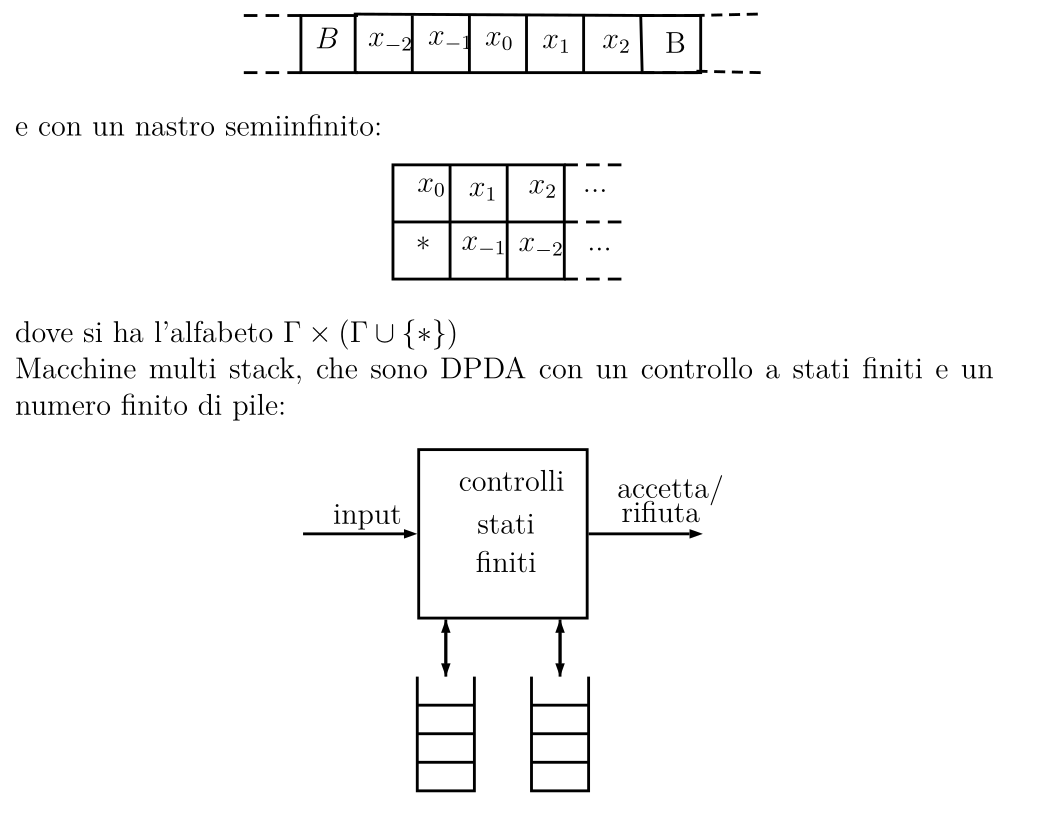
\includegraphics{2025-01-16_15-18.png}
	% \begin{center}

	% 	\psscalebox{1.0 1.0} % Change this value to rescale the drawing.
	% 	{
	% 		\begin{pspicture}(0,-0.43)(7.181278,0.43)
	% 			\psline[linecolor=black, linewidth=0.04](1.5008337,0.39)(1.5008337,-0.41)
	% 			\psline[linecolor=black, linewidth=0.04](2.3008337,0.39)(2.3008337,-0.41)
	% 			\psline[linecolor=black, linewidth=0.04](3.1008337,0.39)(3.1008337,-0.41)
	% 			\psline[linecolor=black, linewidth=0.04](3.9008338,0.39)(3.9008338,-0.41)
	% 			\psline[linecolor=black, linewidth=0.04](4.700834,0.39)(4.700834,-0.41)
	% 			\psline[linecolor=black, linewidth=0.04, linestyle=dashed, dash=0.17638889cm 0.10583334cm](5.5008335,0.39)(6.3008337,0.39)
	% 			\psline[linecolor=black, linewidth=0.04, linestyle=dashed, dash=0.17638889cm 0.10583334cm](5.5008335,-0.41)(6.3008337,-0.41)
	% 			\rput[bl](3.3208337,-0.09){$x_0$}
	% 			\rput[bl](1.6808337,-0.13){$x_{-2}$}
	% 			\rput[bl](2.5208337,-0.11){$x_{-1}$}
	% 			\rput[bl](4.120834,-0.13){$x_1$}
	% 			\rput[bl](4.9608335,-0.13){$x_2$}
	% 			\psline[linecolor=black, linewidth=0.04](1.4808338,0.41)(5.560834,0.39)
	% 			\psline[linecolor=black, linewidth=0.04](1.5008337,-0.41)(5.520834,-0.41)(5.5008335,0.39)
	% 			\psline[linecolor=black, linewidth=0.04](1.5408337,0.39)(0.74083376,0.39)(0.74083376,-0.41)(1.5408337,-0.41)
	% 			\psline[linecolor=black, linewidth=0.04, linestyle=dashed, dash=0.17638889cm 0.10583334cm](0.74083376,0.39)(-0.05916626,0.39)
	% 			\psline[linecolor=black, linewidth=0.04, linestyle=dashed, dash=0.17638889cm 0.10583334cm](0.74083376,-0.41)(-0.05916626,-0.41)
	% 			\rput[bl](0.94083375,-0.07){$B$}
	% 			\psline[linecolor=black, linewidth=0.04, linestyle=dashed, dash=0.17638889cm 0.10583334cm](6.2408338,0.39)(7.140834,0.41)
	% 			\psline[linecolor=black, linewidth=0.04, linestyle=dashed, dash=0.17638889cm 0.10583334cm](6.2808337,-0.39)(7.180834,-0.41)
	% 			\psline[linecolor=black, linewidth=0.04](5.540834,0.39)(6.3408337,0.39)(6.3408337,-0.41)(5.540834,-0.41)
	% 			\rput[bl](5.8408337,-0.13){B}
	% 		\end{pspicture}
	% 	}

	% \end{center}
	% e con un nastro semiinfinito:
	% \begin{center}

	% 	\psscalebox{1.0 1.0} % Change this value to rescale the drawing.
	% 	{
	% 		\begin{pspicture}(0,-0.82)(3.1608338,0.82)
	% 			\psline[linecolor=black, linewidth=0.04](0.02,-0.8)(2.42,-0.8)(2.42,0.8)(0.02,0.8)(0.02,-0.8)(0.82,-0.8)(0.82,0.8)(1.62,0.8)(1.62,-0.8)(2.42,-0.8)(2.42,0.0)(0.02,0.0)
	% 			\psline[linecolor=black, linewidth=0.04, linestyle=dashed, dash=0.17638889cm 0.10583334cm](2.42,0.8)(3.22,0.8)
	% 			\psline[linecolor=black, linewidth=0.04, linestyle=dashed, dash=0.17638889cm 0.10583334cm](2.42,0.0)(3.22,0.0)
	% 			\psline[linecolor=black, linewidth=0.04, linestyle=dashed, dash=0.17638889cm 0.10583334cm](2.42,-0.8)(3.22,-0.8)
	% 			\rput[bl](0.36,0.36){$x_0$}
	% 			\rput[bl](1.08,0.3){$x_1$}
	% 			\rput[bl](1.92,0.34){$x_2$}
	% 			\rput[bl](2.68,0.42){$...$}
	% 			\rput[bl](0.34,-0.52){*}
	% 			\rput[bl](0.98,-0.48){$x_{-1}$}
	% 			\rput[bl](1.78,-0.5){$x_{-2}$}
	% 			\rput[bl](2.74,-0.4){...}
	% 		\end{pspicture}
	% 	}

	% \end{center}
	% dove si ha l'alfabeto $\Gamma\times (\Gamma\cup\{*\})$\\
	% Macchine multi stack, che sono DPDA con un controllo a stati finiti e un numero finito di pile:
	% \begin{center}
	% 	\psscalebox{1.0 1.0} % Change this value to rescale the drawing.
	% 	{
	% 		\begin{pspicture}(0,-2.41)(5.64,2.41)
	% 			\psframe[linecolor=black, linewidth=0.04, dimen=outer](4.0,2.41)(1.6,0.01)
	% 			\psline[linecolor=black, linewidth=0.04, arrowsize=0.05291667cm 2.0,arrowlength=1.4,arrowinset=0.0]{->}(0.0,1.21)(1.6,1.21)
	% 			\psline[linecolor=black, linewidth=0.04, arrowsize=0.05291667cm 2.0,arrowlength=1.4,arrowinset=0.0]{->}(4.0,1.21)(5.6,1.21)
	% 			\psline[linecolor=black, linewidth=0.04, arrowsize=0.05291667cm 2.0,arrowlength=1.4,arrowinset=0.0]{->}(2.0,0.01)(2.0,-0.79)
	% 			\psline[linecolor=black, linewidth=0.04, arrowsize=0.05291667cm 2.0,arrowlength=1.4,arrowinset=0.0]{->}(2.0,-0.79)(2.0,0.01)
	% 			\psline[linecolor=black, linewidth=0.04, arrowsize=0.05291667cm 2.0,arrowlength=1.4,arrowinset=0.0]{->}(3.6,0.01)(3.6,-0.79)
	% 			\psline[linecolor=black, linewidth=0.04, arrowsize=0.05291667cm 2.0,arrowlength=1.4,arrowinset=0.0]{->}(3.6,-0.79)(3.6,0.01)
	% 			\psline[linecolor=black, linewidth=0.04](1.6,-0.79)(1.6,-2.39)(2.4,-2.39)(2.4,-0.79)(2.4,-1.19)(1.6,-1.19)(1.6,-1.59)(2.4,-1.59)(2.4,-1.99)(1.6,-1.99)(2.4,-1.99)
	% 			\psline[linecolor=black, linewidth=0.04](3.2,-0.79)(3.2,-2.39)(4.0,-2.39)(4.0,-0.79)(4.0,-1.19)(3.2,-1.19)(3.2,-1.59)(4.0,-1.59)(4.0,-1.99)(3.2,-1.99)(4.0,-1.99)
	% 			\rput[bl](0.42,1.27){input}
	% 			\rput[bl](4.4,1.61){accetta/}
	% 			\rput[bl](4.46,1.37){rifiuta}
	% 			\rput[bl](2.18,1.81){controlli}
	% 			\rput[bl](2.44,1.21){stati}
	% 			\rput[bl](2.42,0.67){finiti}
	% 		\end{pspicture}
	% 	}
	% \end{center}
	e si ha:
	$$\delta(q,a,x_1,x_2,...,x_k)=(p,\gamma_1,\gamma_2,...,\gamma_k)$$
	% \begin{example}
	% 	Legge l'input e lo spinge tutto sul primo stack (sfruttando un simbolo ausiliario di fine input):
	% 	\begin{center}
	% 		\psscalebox{1.0 1.0} % Change this value to rescale the drawing.
	% 		{
	% 			\begin{pspicture}(0,-2.98)(4.02,2.98)
	% 				\psframe[linecolor=black, linewidth=0.04, dimen=outer](4.0,2.98)(1.6,0.58)
	% 				\psline[linecolor=black, linewidth=0.04, arrowsize=0.05291667cm 2.0,arrowlength=1.4,arrowinset=0.0]{->}(0.0,1.78)(1.6,1.78)
	% 				\psline[linecolor=black, linewidth=0.04, arrowsize=0.05291667cm 2.0,arrowlength=1.4,arrowinset=0.0]{->}(2.0,0.58)(2.0,-0.22)
	% 				\psline[linecolor=black, linewidth=0.04, arrowsize=0.05291667cm 2.0,arrowlength=1.4,arrowinset=0.0]{->}(2.0,-0.22)(2.0,0.58)
	% 				\psline[linecolor=black, linewidth=0.04, arrowsize=0.05291667cm 2.0,arrowlength=1.4,arrowinset=0.0]{->}(3.6,0.58)(3.6,-0.22)
	% 				\psline[linecolor=black, linewidth=0.04, arrowsize=0.05291667cm 2.0,arrowlength=1.4,arrowinset=0.0]{->}(3.6,-0.22)(3.6,0.58)
	% 				\psline[linecolor=black, linewidth=0.04](1.6,-0.22)(1.6,-1.82)(2.4,-1.82)(2.4,-0.22)(2.4,-0.62)(1.6,-0.62)(1.6,-1.02)(2.4,-1.02)(2.4,-1.42)(1.6,-1.42)(2.4,-1.42)
	% 				\psline[linecolor=black, linewidth=0.04](3.2,-0.22)(3.2,-1.82)(4.0,-1.82)(4.0,-0.22)(4.0,-0.62)(3.2,-0.62)(3.2,-1.02)(4.0,-1.02)(4.0,-1.42)(3.2,-1.42)(4.0,-1.42)
	% 				\rput[bl](0.42,1.84){input}
	% 				\rput[bl](1.94,-0.44){a}
	% 				\rput[bl](1.92,-0.88){s}
	% 				\rput[bl](1.92,-1.28){a}
	% 				\rput[bl](1.92,-1.72){c}
	% 				\rput[bl](3.5,-0.44){c}
	% 				\rput[bl](3.5,-0.92){a}
	% 				\rput[bl](3.56,-1.3){s}
	% 				\rput[bl](3.56,-1.68){a}
	% 				\psline[linecolor=black, linewidth=0.04](1.6,-1.82)(1.6,-2.22)(2.4,-2.22)(2.4,-1.82)
	% 				\psline[linecolor=black, linewidth=0.04](3.2,-1.82)(3.2,-2.22)(4.0,-2.22)(4.0,-1.82)
	% 				\rput[bl](1.8,-2.14){$z_0$}
	% 				\rput[bl](3.44,-2.2){$z_0$}
	% 				\rput[bl](0.36,1.42){$casa\$$}
	% 				\psline[linecolor=black, linewidth=0.04](2.0,-2.22)(2.0,-2.62)
	% 				\psline[linecolor=black, linewidth=0.04](3.6,-2.62)(3.6,-2.22)
	% 				\psline[linecolor=black, linewidth=0.04](2.0,-2.62)(3.6,-2.62)
	% 				\rput[bl](2.26,-2.98){ribalto}
	% 				\psline[linecolor=black, linewidth=0.04, arrowsize=0.05291667cm 2.0,arrowlength=1.4,arrowinset=0.0]{->}(3.6,-2.62)(3.6,-2.22)
	% 			\end{pspicture}
	% 		}

	% 	\end{center}
	%\end{example}
	si ha un'ulteriore restrizione:
	Supponiamo che i simboli sulle pile possano essere solo $x$ o
$z_0$. Si riescono ancora a simulare le macchine di Turing
			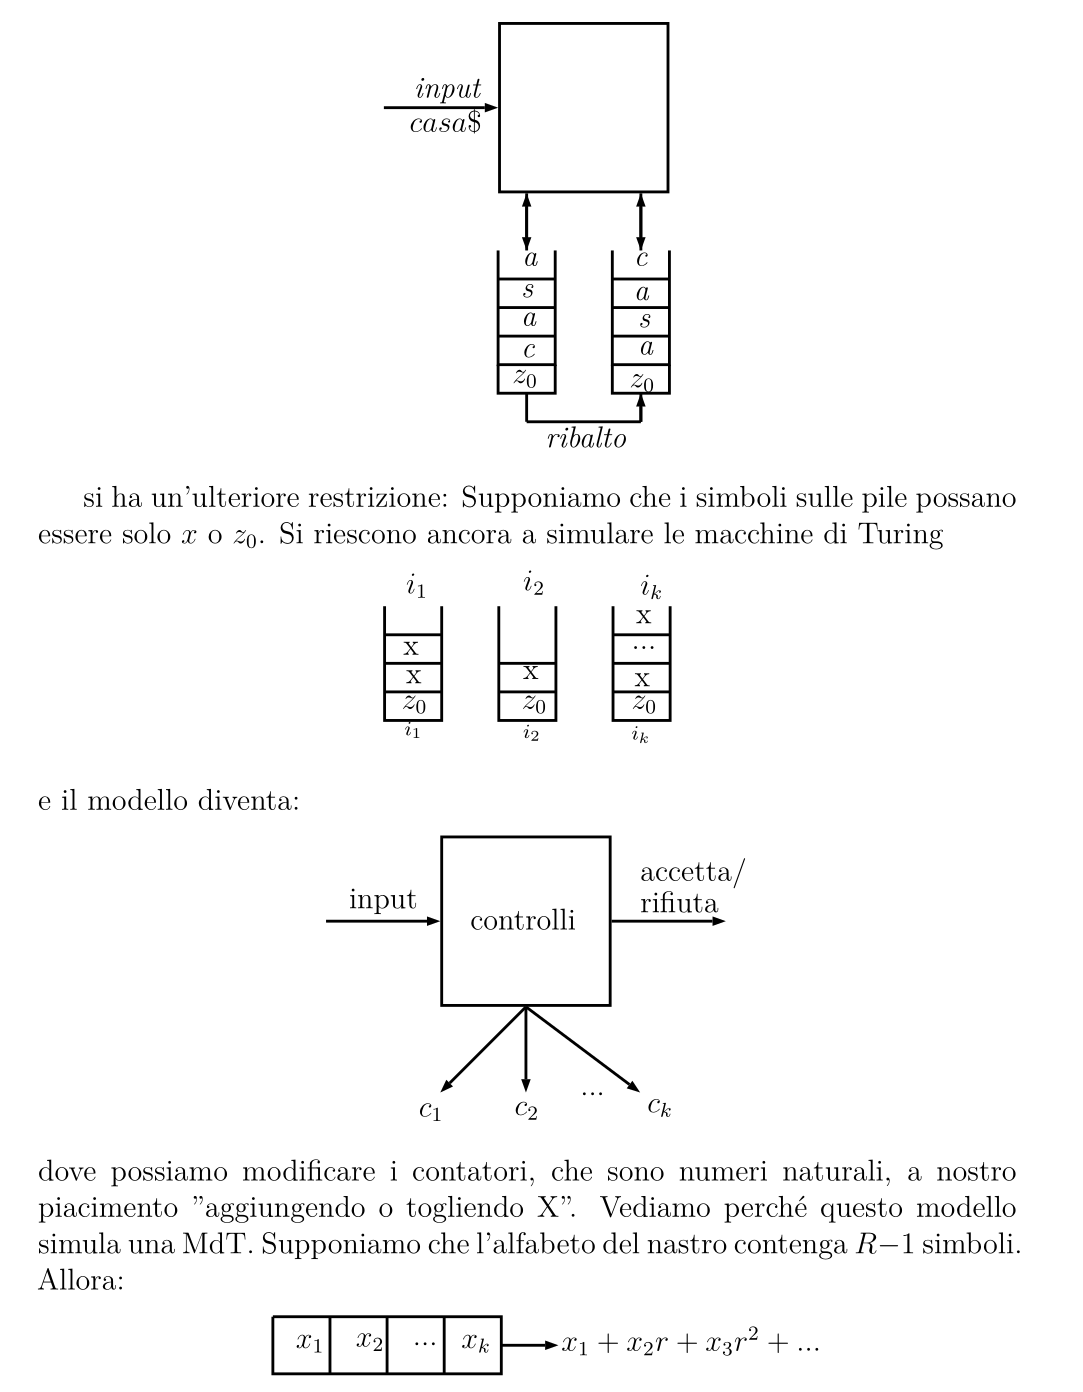
\includegraphics{2025-01-16_15-19.png}


% \begin{center}
% 		\psscalebox{1.0 1.0} % Change this value to rescale the drawing.
% 		{
% 			\begin{pspicture}(0,-1.23)(4.04,1.23)
% 				\psline[linecolor=black, linewidth=0.04](0.02,0.79)(0.02,-0.81)(0.82,-0.81)(0.82,0.79)(0.82,0.39)(0.02,0.39)
% 				\psline[linecolor=black, linewidth=0.04](0.02,-0.01)(0.82,-0.01)
% 				\psline[linecolor=black, linewidth=0.04](0.02,-0.41)(0.82,-0.41)
% 				\psline[linecolor=black, linewidth=0.04](1.62,0.79)(1.62,-0.81)(2.42,-0.81)(2.42,0.79)
% 				\psline[linecolor=black, linewidth=0.04](1.62,-0.01)(2.42,-0.01)
% 				\psline[linecolor=black, linewidth=0.04](1.62,-0.41)(2.42,-0.41)
% 				\psline[linecolor=black, linewidth=0.04](3.22,0.79)(3.22,-0.81)(4.02,-0.81)(4.02,0.79)(4.02,0.39)(3.22,0.39)
% 				\psline[linecolor=black, linewidth=0.04](3.22,-0.01)(4.02,-0.01)
% 				\psline[linecolor=black, linewidth=0.04](3.22,-0.41)(4.02,-0.41)
% 				\rput[bl](0.32,0.91){$i_1$}
% 				\rput[bl](0.28,0.11){x}
% 				\rput[bl](0.32,-0.29){x}
% 				\rput[bl](0.26,-0.71){$z_0$}
% 				\rput[bl](1.96,-0.23){x}
% 				\rput[bl](1.94,-0.71){$z_0$}
% 				\rput[bl](3.54,0.55){x}
% 				\rput[bl](3.48,0.19){...}
% 				\rput[bl](3.52,-0.33){x}
% 				\rput[bl](3.48,-0.71){$z_0$}
% 				\rput[bl](1.96,0.95){$i_2$}
% 				\rput[bl](3.6,0.89){$i_k$}
% 				\rput[bl](0.3,-1.17){$^{i_1}$}
% 				\rput[bl](1.96,-1.21){$^{i_2}$}
% 				\rput[bl](3.48,-1.23){$^{i_k}$}
% 			\end{pspicture}
% 		}
% 	\end{center}
% 	e il modello diventa:
% 	\begin{center}


% 		\psscalebox{1.0 1.0} % Change this value to rescale the drawing.
% 		{
% 			\begin{pspicture}(0,-2.0)(5.64,2.0)
% 				\psframe[linecolor=black, linewidth=0.04, dimen=outer](4.0,2.0)(1.6,-0.4)
% 				\psline[linecolor=black, linewidth=0.04, arrowsize=0.05291667cm 2.0,arrowlength=1.4,arrowinset=0.0]{->}(0.0,0.8)(1.6,0.8)
% 				\psline[linecolor=black, linewidth=0.04, arrowsize=0.05291667cm 2.0,arrowlength=1.4,arrowinset=0.0]{->}(4.0,0.8)(5.6,0.8)
% 				\psline[linecolor=black, linewidth=0.04, arrowsize=0.05291667cm 2.0,arrowlength=1.4,arrowinset=0.0]{->}(2.8,-0.4)(1.6,-1.6)
% 				\psline[linecolor=black, linewidth=0.04, arrowsize=0.05291667cm 2.0,arrowlength=1.4,arrowinset=0.0]{->}(2.8,-0.4)(2.8,-1.6)
% 				\psline[linecolor=black, linewidth=0.04, arrowsize=0.05291667cm 2.0,arrowlength=1.4,arrowinset=0.0]{->}(2.8,-0.4)(4.4,-1.6)
% 				\rput[bl](0.32,0.9){input}
% 				\rput[bl](2.02,0.68){controlli}
% 				\rput[bl](4.4,1.26){accetta/}
% 				\rput[bl](4.4,0.92){rifiuta}
% 				\rput[bl](1.3,-2.0){$c_1$}
% 				\rput[bl](2.64,-1.98){$c_2$}
% 				\rput[bl](3.56,-1.64){...}
% 				\rput[bl](4.5,-1.94){$c_k$}
% 			\end{pspicture}
% 		}

% 	\end{center}
% 	dove possiamo modificare i contatori, che sono numeri naturali, a nostro piacimento "aggiungendo
% 	o togliendo X". Vediamo perché questo modello simula una MdT.
% 	Supponiamo che l'alfabeto del nastro contenga $R-1$ simboli. Allora:
% 	\begin{center}

% 		\psscalebox{1.0 1.0} % Change this value to rescale the drawing.
% 		{
% 			\begin{pspicture}(0,-0.42)(7.17,0.42)
% 				\psline[linecolor=black, linewidth=0.04](0.02,0.4)(0.02,0.4)(3.22,0.4)(3.22,-0.4)(0.02,-0.4)(0.02,0.4)
% 				\psline[linecolor=black, linewidth=0.04](0.82,0.4)(0.82,-0.4)
% 				\psline[linecolor=black, linewidth=0.04](1.62,0.4)(1.62,-0.4)
% 				\psline[linecolor=black, linewidth=0.04](2.42,0.4)(2.42,-0.4)
% 				\psline[linecolor=black, linewidth=0.04, arrowsize=0.05291667cm 2.0,arrowlength=1.4,arrowinset=0.0]{->}(3.22,0.0)(4.02,0.0)
% 				\rput[bl](0.34,-0.1){$x_1$}
% 				\rput[bl](1.18,-0.08){$x_2$}
% 				\rput[bl](1.98,0.0){...}
% 				\rput[bl](2.66,-0.1){$x_k$}
% 				\rput[bl](4.06,-0.14){$x_1+x_2r+x_3r^2+...$}
% 			\end{pspicture}
% 		}

% 	\end{center}
	Così come codifico il nastro posso codificare una pila. Per togliere $x_1$ in cima alla pila devo dividere
	il numero per R e prendere il resto. Per aggiungere un nuovo simbolo, moltiplico per R e aggiungo il
	nuovo simbolo. Per modificare il simbolo, basta aggiungere la differenza tra il nuovo e la cima precedente. È immediato farlo con tre contatori (usandone uno di appoggio).
	Per fare tutto ciò bastano due contatori (e quindi due pile) dove nel primo è codificato come:
	$$2^{c_1}3^{c_2}5^{c_3}$$
	Per i linguaggi si ha quindi:
	\begin{itemize}
		\item linguaggi ricorsivi $\to$ decidibili e MdT si ferma sempre
		\item linguaggi ricorsivamente enumerabili $\to$ semidecidibili (ma comunque indecidibili) e MdT si ferma se accetta ma potrebbe non fermarsi
		\item linguaggi non ricorsivamente enumerabili $\to$ indecidibili e $\not\exists$ MdT
	\end{itemize}
	quindi, insiemisticamente:
	\begin{center}
			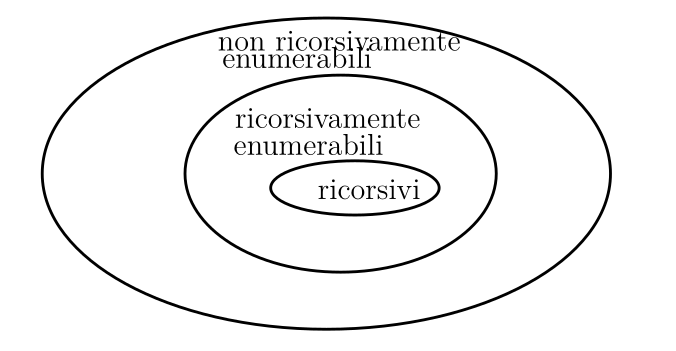
\includegraphics{2025-01-16_15-21.png}

		% \psscalebox{1.0 1.0} % Change this value to rescale the drawing.
		% {
		% 	\begin{pspicture}(0,-2.2)(8.0,2.2)
		% 		\psellipse[linecolor=black, linewidth=0.04, dimen=outer](4.0,0.0)(4.0,2.2)
		% 		\psellipse[linecolor=black, linewidth=0.04, dimen=outer](4.2,0.0)(2.2,1.4)
		% 		\psellipse[linecolor=black, linewidth=0.04, dimen=outer](4.4,-0.2)(1.2,0.4)
		% 		\rput[bl](2.48,1.72){non ricorsivamente }
		% 		\rput[bl](2.72,0.64){ricorsivamente }
		% 		\rput[bl](3.88,-0.36){ricorsivi}
		% 		\rput[bl](2.7,0.26){enumerabili}
		% 		\rput[bl](2.54,1.48){enumerabili}
		% 	\end{pspicture}
		% }

	\end{center}
	\begin{example}
		vediamo un linguaggio non ricorsivamente enumerabile.\\
		$w\in\{o,1\}^*$ biiezione tra stringhe e numeri:
		\begin{center}
			\begin{tabular}{c c c c c c c}
				$w_1$         & $w_2$ & $w_3$ & $w_4$ & $w_5$ & $w_6$ & ... \\
				1             & 2     & 3     & 4     & 5     & 6     & ... \\
				$\varepsilon$ & 0     & 1     & 00    & 01    & 10    & ..
			\end{tabular}
		\end{center}
		Consideriamo però le due stringe 00101 e 0101: se le leggessi come numeri binari sono entrambi
		5, quindi abbiamo perso la biiezione.
		Forziamo quindi l'interpretazione delle stringhe mettendoci davanti un 1.
		Codifichiamo anche una MdT in binario:
		$$M=(Q,\{0,1\},\Gamma,\delta,q_1,B,\{q_2\})$$
		$$Q=\{q_1,...,q_r\}$$
		$$\Gamma=\{x_1,...,x_s\}=\{0,1,B,...\}$$
		$$direzioni:\,\,L\to D_1\,\,R\to D_2$$
		$$\underbrace{\delta(q_i,x_j)=(q_k,x_1,D_m}_{0^i10^j10^k10^l10^m}$$
		$$Cod_111Cod_211Cod_3\\...=Cpd(\delta)$$
	\end{example}
	\begin{example}
		sia $M=(\{q_1,q_2,q_3\},\{o,1\}.\{0,1,B\},\delta,q_1,B,q_2)$ con:
		$$\overbrace{0}^{q_1}1\overbrace{00}^{x_2}1\overbrace{000}^{q_3}1\overbrace{0}^{x_1}1\overbrace{00}^{D_2}$$
		$$\delta(q_1,1)=(q_3,0,R)$$
		$$\delta(q_3,0)=(q_1,1,R)$$
		$$\delta(q_3,1)=(q_2,0,R)$$
		$$\delta(q_3,B)=(q_3,1,L)$$
		Quindi ora possiamo dire che M è Mi, ovvero l'i-esima macchina di Turing.
		\\
		si ha però un problema: io posso permutare le delta, ottenendo numeri diversi, pur descrivendo la stessa
		macchina. Quindi la stessa macchina compare più volte nella sequenza infinita. Inoltre, data una
		stringa, non è detto che rappresenti una MdT. Inoltre:
		$$Cod((M,W))=Cod(M)111Cod(W)$$
		definisco quindi $L_d$
		$$L_d=\{w_i\in\{0,1\}^*|\,w_L\in L(M_i)\}$$
		e considero la tabella infinita:
		\begin{center}
			\begin{tabular}{c c|c c c c c c}
				       &   &          &          & j        &          &                \\
				       & 1 & 2        & 3        & 4        & 5        & 6              \\
				\hline
				       & 1 & 0        & 1        & 1        & 0        & ... & ...      \\
				       & 2 & 1        & 1        & 0        & 0        & ... & ...      \\
				       & 3 & 0        & 0        & 1        & 1        & ... & ...      \\
				(Mi) i & 4 & 0        & 1        & 0        & 1        & ... & ...      \\
				       & 5 & $\vdots$ & $\vdots$ & $\vdots$ & $\vdots$ & ... & ...      \\
				       & 6 & $\vdots$ & $\vdots$ & $\vdots$ & $\vdots$ & ... & $\ddots$
			\end{tabular}
		\end{center}
		Osserviamo la diagonale della tabella. Fanno parte di Ld solo le stringhe che hanno 0 sulla
		diagonale. Prendo in sostanza il complemento della diagonale.
		Se esistesse una MdT accettante, allora esisterebbe una riga uguale a tale complemento.
		Però tale complemento non è uguale a nessuna delle righe, perché differisce per l'i-esimo valore
		dall'i-esima riga (essendo il negato di tale valore!).
	\end{example}
	\begin{theorem}
		Se L è ricorsivo, allora il complementare di L è ricorsivo.
	\end{theorem}
	\begin{proof}
		Se L è ricorsivo, allora esiste una MdT M tale che $L = L(M)$. Costruiamo $M^{'}$ tale che
		$L(M^{'}$ = complementare di L.
	\end{proof}
	\begin{theorem}
		$$L,\overline{L}\in RE\to L,\overline{L}\in RIC$$
		se un linguaggio e il suo complementare sono ricorsivamente enumerabili allora quel linguaggio è ricorsivo
	\end{theorem}
	\begin{proof}
		$$L\in RE\to \exists M_L\to L=L(M_L)$$
		$$\overbrace{L}\in RE\to \exists M_{\overline{L}}\to \overline{L}=L(M_L)$$
	\end{proof}
	Poiché ogni stringa o appartiene a L o al complemento di L, costruiamo una nuova macchina M che
	simula $M_L$ e $M_{\overline{L}}$˛\\Prima o poi una delle due macchina deve fermarsi. Allora possiamo accettare o rifiutare.\\
	Si ha quindi la seguente tabella per i vari casi:
	\begin{center}
		\begin{tabular}{c c c c }
			accettabile & Ric              & RE               & non RE           \\
			\hline
			si          & $L,\overline{L}$ &                  &                  \\
			no          & $L$              & $\overline{L}$   &                  \\
			no          & $L$              &                  & $\overline{L}$   \\
			no          & $\overline{L}$   & $L$              &                  \\
			no          &                  & $L,\overline{L}$ &                  \\
			si          &                  & $L$              & $\overline{L}$   \\
			no          & $\overline{L}$   &                  & $L$              \\
			si          &                  & $\overline{L}$   & $L$              \\
			si          &                  &                  & $L,\overline{L}$ \\
		\end{tabular}
	\end{center}
	\section{Macchina di Turing Universale}
	Abbiamo già visto che si può codificare in binario una MdT, possiamo codificare anche la coppia
	MdT con il suo input:
	$$Cod(M)111Cod(M)\,\,[M111W]$$Possiamo quindi pensare a una MdT universale che sappia simulare qualsiasi altra MdT specificata come da codifica:
			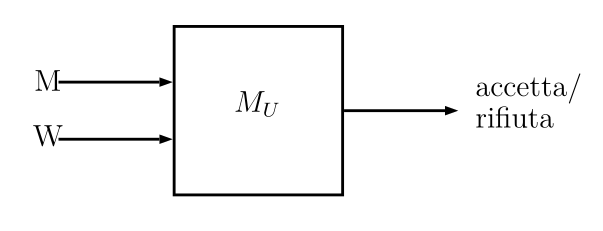
\includegraphics{2025-01-16_15-22.png}

	% \begin{center}
	% 	\psscalebox{1.0 1.0} % Change this value to rescale the drawing.
	% 	{
	% 		\begin{pspicture}(0,-1.2)(7.44,1.2)
	% 			\psframe[linecolor=black, linewidth=0.04, dimen=outer](4.36,1.2)(1.96,-1.2)
	% 			\psline[linecolor=black, linewidth=0.04, arrowsize=0.05291667cm 2.0,arrowlength=1.4,arrowinset=0.0]{->}(0.36,0.4)(1.96,0.4)
	% 			\psline[linecolor=black, linewidth=0.04, arrowsize=0.05291667cm 2.0,arrowlength=1.4,arrowinset=0.0]{->}(0.36,-0.4)(1.96,-0.4)
	% 			\psline[linecolor=black, linewidth=0.04, arrowsize=0.05291667cm 2.0,arrowlength=1.4,arrowinset=0.0]{->}(4.36,0.0)(5.96,0.0)
	% 			\rput[bl](0.02,0.28){M}
	% 			\rput[bl](0.0,-0.5){W}
	% 			\rput[bl](2.82,-0.08){$M_U$}
	% 			\rput[bl](6.2,0.1){accetta/}
	% 			\rput[bl](6.2,-0.24){rifiuta}
	% 		\end{pspicture}
	% 	}
	% \end{center}
	$$L_U\{(M,W)|W\in L(M)\}$$
	La macchina universale corrisponde alla nostra idea di computer programmabile. Descriviamo
	questa macchina universale, che ha quattro nastri:
	\begin{itemize}
		\item \textbf{primo nastro:} $M111W$
		\item \textbf{secondo nastro:} nastro/codifica di M
		\item \textbf{terzo nastro:} stato/codifica di M
		\item \textbf{quarto nastro:} ausiliario

	\end{itemize}
	Il linguaggio universale è ricorsivamente enumerabile ma non ricorsivo (non potrebbe esserlo, visto
	che la macchina che simula potrebbe non fermarsi).
	Il diagramma delle classi dei linguaggi è quindi diventato il seguente:
			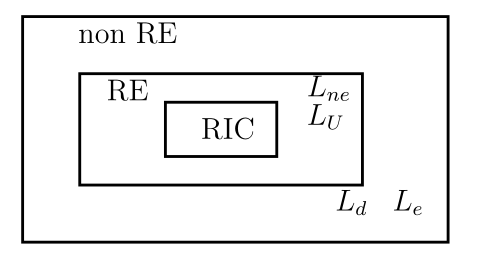
\includegraphics{2025-01-16_15-23.png}
	% \begin{center}
	% 	\psscalebox{1.0 1.0} % Change this value to rescale the drawing.
	% 	{
	% 		\begin{pspicture}(0,-1.6)(6.0,1.6)
	% 			\psframe[linecolor=black, linewidth=0.04, dimen=outer](6.0,1.6)(0.0,-1.6)
	% 			\psframe[linecolor=black, linewidth=0.04, dimen=outer](4.8,0.8)(0.8,-0.8)
	% 			\psframe[linecolor=black, linewidth=0.04, dimen=outer](3.6,0.4)(2.0,-0.4)
	% 			\rput[bl](0.8,1.2){non RE}
	% 			\rput[bl](1.2,0.4){RE}
	% 			\rput[bl](2.52,-0.14){RIC}
	% 			\rput[bl](4.0,0.4){$L_{ne}$}
	% 			\rput[bl](4.0,0.0){$L_U$}
	% 			\rput[bl](5.2,-1.2){$L_e$}
	% 			\rput[bl](4.4,-1.2){$L_d$}
	% 		\end{pspicture}
	% 	}
	% \end{center}
	Valgono ancora le riduzioni. Sapendo che $P_1$ è indecidibile (non RE o RE), posso fare una riduzione
	dalle istanze di $P_1$  alle istanze di $P_2$ mostrando che $P_2$ è indecidibile.
	Con la riduzione stiamo dicendo che $P_2$ è almeno difficile quanto $P_1$  (e non viceversa!).
	Notiamo che non è nemmeno necessario che tutte le istanze di $P_2$  siano "coperte" dal processo di
riduzione.
\begin{theorem}
	$$L_{ne}\in RE$$
\end{theorem}
\begin{proof}
	Dobbiamo fare una riduzione da $L_u$ a $L_{ne}$ per mostrare che $L_{ne}$ è ricorsivamente enumerabile.
	La riduzione è descritta da questo schema:
	\begin{center}
			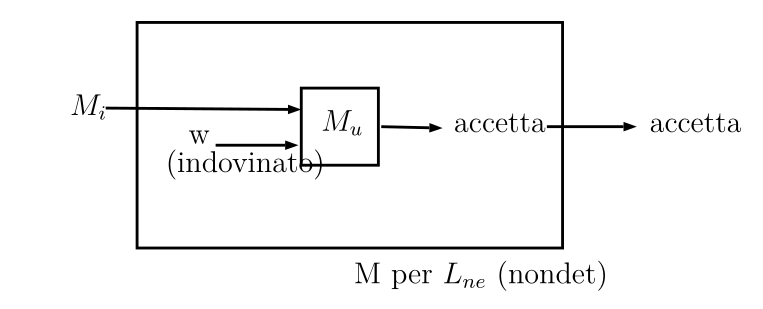
\includegraphics{2025-01-16_15-25.png}
		% \psscalebox{1.0 1.0} % Change this value to rescale the drawing.
		% {
		% 	\begin{pspicture}(0,-1.89)(9.2,1.89)
		% 		\psframe[linecolor=black, linewidth=0.04, dimen=outer](6.92,1.89)(0.92,-1.31)
		% 		\psframe[linecolor=black, linewidth=0.04, dimen=outer](4.34,0.97)(3.22,-0.15)
		% 		\psline[linecolor=black, linewidth=0.04, arrowsize=0.05291667cm 2.0,arrowlength=1.4,arrowinset=0.0]{->}(0.5,0.67)(3.24,0.65)
		% 		\psline[linecolor=black, linewidth=0.04, arrowsize=0.05291667cm 2.0,arrowlength=1.4,arrowinset=0.0]{->}(2.04,0.15)(3.2,0.15)
		% 		\psline[linecolor=black, linewidth=0.04, arrowsize=0.05291667cm 2.0,arrowlength=1.4,arrowinset=0.0]{->}(4.36,0.41)(5.22,0.39)
		% 		\psline[linecolor=black, linewidth=0.04, arrowsize=0.05291667cm 2.0,arrowlength=1.4,arrowinset=0.0]{->}(6.68,0.41)(7.94,0.41)
		% 		\rput[bl](5.38,0.33){accetta}
		% 		\rput[bl](8.12,0.33){accetta}
		% 		\rput[bl](1.66,0.17){w}
		% 		\rput[bl](1.34,-0.33){(indovinato)}
		% 		\rput[bl](0.0,0.51){$M_i$}
		% 		\rput[bl](3.52,0.29){$M_u$}
		% 		\rput[bl](3.98,-1.89){M per $L_{ne}$ (nondet)}
		% 	\end{pspicture}
		% }
	\end{center}
\end{proof}
\begin{theorem}
	$$L_{ne}\not\in RIC$$
\end{theorem}
\begin{proof}
	infatti essendo $l_e$ il complementare di $l_{ne}$, per i teoremi visti in precedenza  $l_e$ non può essere ricorsivo
	né può essere ricorsivamente enumerabile. Segue che  $l_e$ è non RE
\end{proof}
\begin{example}
	considero:
	$$L_e=\{M|\,L(M)=\emptyset\}$$
	$$L_{ne}=\{M|\,L(M)=\emptyset\}$$
\end{example}
%%% Local Variables:
%%% mode: LaTeX
%%% TeX-master: ../libro-linguaggi
%%% End:



\parte{Parser}\label{part:parser}
%%% Local Variables:
%%% mode: LaTeX
%%% TeX-master: "../libro-linguaggi"
%%% End:

\section{Parser Top-down}\label{sec:parser-top-down}

L'idea intuitiva dei \textbf{parser top-down} è estremamente semplice: costruire l'albero di derivazione a partire da un albero $D$ formato dalla
sola radice ed estendere l'albero con l'espansione di una produzione alla volta, finchè non si ottiene esattamente il
testo $T$.

Questa tipologia di parser si contrappone a quella dei \textbf{parser bottom-up} che invece partono dall'analisi del
testo e costruiscono l'albero di derivazione partendo dalle foglie, finchè non viene ricostruita la radice dell'albero.
Questa tipologia era dominante in passato, quando i computer erano decisamente meno potenti e procedure efficienti, ma
complesse, erano necessarie per effettuare il parsing in tempi ragionevoli.
Negli ultimi anni si vede invece una tendenza verso i parser top-down, in quanto gli algoritmi utilizzati sono semplici,
sia da descrivere che da implementare, sebbene non abbiano le stesse garanzie di efficienza di alcuni parser bottom-up.



%%% Local Variables:
%%% mode: LaTeX
%%% TeX-master: "../libro-linguaggi"
%%% TeX-engine: luatex
%%% End:

\section{Parser LL}

%%% Local Variables:
%%% mode: LaTeX
%%% TeX-master: "../libro-linguaggi"
%%% TeX-engine: luatex
%%% End:

\section{Parser LR\($k$\)}

\section{Parsing  Expression Grammars}



%\appendix % From here onwards, chapters are numbered with letters, as is the appendix convention

%\parte{Appendix}

%\input{chapters/appendix.tex}

%----------------------------------------------------------------------------------------

\backmatter % Denotes the end of the main document content
\setchapterstyle{plain} % Output plain chapters from this point onwards

%----------------------------------------------------------------------------------------
%       BIBLIOGRAPHY
%----------------------------------------------------------------------------------------

% The bibliography needs to be compiled with biber using your LaTeX editor, or on the command line with 'biber main' from the template directory

%\defbibnote{bibnote}{Here are the references in citation order.\par\bigskip} % Prepend this text to the bibliography
\printbibliography[heading=bibintoc, title=Bibliografia] % Add the bibliography heading to the ToC, set the title of the bibliography and output the bibliography note


%----------------------------------------------------------------------------------------
%       NOMENCLATURE
%----------------------------------------------------------------------------------------

% The nomenclature needs to be compiled on the command line with 'makeindex main.nlo -s nomencl.ist -o main.nls' from the template directory

\nomenclature{$A$, $B$}{Insieme generico}
\nomenclature{$\Sigma$}{Alfabeto}
\nomenclature{$w, x, y, z$}{Parole o stringhe}
\nomenclature{$\epsilon$}{Parola vuota}
\nomenclature{$L$}{Linguaggio}
%\nomenclature{$h$}{Planck constant}
%
\renewcommand{\nomname}{Lista dei simboli} % Rename the default 'Nomenclature'
\renewcommand{\nompreamble}{Lista dei simboli.} % Prepend this text to the nomenclature
%
\printnomenclature% Output the nomenclature


%----------------------------------------------------------------------------------------
%       GLOSSARY
%----------------------------------------------------------------------------------------

% The glossary needs to be compiled on the command line with 'makeglossaries main' from the template directory
%
%\setglossarystyle{listgroup} % Set the style of the glossary (see https://en.wikibooks.org/wiki/LaTeX/Glossary for a reference)
%\printglossary[title=Special Terms, toctitle=List of Terms] % Output the glossary, 'title' is the chapter heading for the glossary, toctitle is the table of contents heading

%----------------------------------------------------------------------------------------
%       INDEX
%----------------------------------------------------------------------------------------

% The index needs to be compiled on the command line with 'makeindex main' from the template directory

%\printindex % Output the index

\end{document}

%%% Local Variables:
%%% mode: LaTeX
%%% TeX-engine: luatex
%%% End:
